%%% The main file. It contains definitions of basic parameters and includes all other parts.

%% Settings for single-side (simplex) printing
% Margins: left 40mm, right 25mm, top and bottom 25mm
% (but beware, LaTeX adds 1in implicitly)
\documentclass[12pt,a4paper]{report}
\setlength\textwidth{145mm}
\setlength\textheight{247mm}
\setlength\oddsidemargin{15mm}
\setlength\evensidemargin{15mm}
\setlength\topmargin{0mm}
\setlength\headsep{0mm}
\setlength\headheight{0mm}
% \openright makes the following text appear on a right-hand page
\let\openright=\clearpage

%% Settings for two-sided (duplex) printing
% \documentclass[12pt,a4paper,twoside,openright]{report}
% \setlength\textwidth{145mm}
% \setlength\textheight{247mm}
% \setlength\oddsidemargin{14.2mm}
% \setlength\evensidemargin{0mm}
% \setlength\topmargin{0mm}
% \setlength\headsep{0mm}
% \setlength\headheight{0mm}
% \let\openright=\cleardoublepage

%% Generate PDF/A-2u
\usepackage[a-2u]{pdfx}

%% Character encoding: usually latin2, cp1250 or utf8:
\usepackage[utf8]{inputenc}

%% Prefer Latin Modern fonts
\usepackage{lmodern}

%% Further useful packages (included in most LaTeX distributions)
\usepackage{amsmath}        % extensions for typesetting of math
\usepackage{amsfonts}       % math fonts
\usepackage{amsthm}         % theorems, definitions, etc.
\usepackage{bbding}         % various symbols (squares, asterisks, scissors, ...)
\usepackage{bm}             % boldface symbols (\bm)
\usepackage{graphicx}       % embedding of pictures
\usepackage{fancyvrb}       % improved verbatim environment
\usepackage[sort&compress,numbers]{natbib}         % citation style AUTHOR (YEAR), or AUTHOR [NUMBER]
\usepackage[nottoc]{tocbibind} % makes sure that bibliography and the lists
			    % of figures/tables are included in the table
			    % of contents
\usepackage{dcolumn}        % improved alignment of table columns
\usepackage{booktabs}       % improved horizontal lines in tables
\usepackage{paralist}       % improved enumerate and itemize
\usepackage{xcolor}         % typesetting in color

\usepackage{dsfont}
\usepackage{braket}
\usepackage{tikz} % Export grafů z RStudia
\usepackage{float} %použití [H] u figur, umístění na přesné místo
\usepackage{mathtools} %pro \dcases
\usepackage{subcaption}
\usepackage{bbm}

\usetikzlibrary{arrows} 
\usepackage{subcaption}
% \usepackage{xcolor}

%\usepackage{array}
%\usepackage{dsfont}

% \usepackage{amsmath}        % rozšíření pro sazbu matematiky
% \usepackage{amssymb}        %přidáno, pokud se něco kazí, tak to může být tímto----------------------------------------------
% \usepackage{amsfonts}       % matematické fonty
% \usepackage{amsthm}         % sazba vět, definic apod.
% \usepackage{bbding}         % balíček s nejrůznějšími symboly
% 			    % (čtverečky, hvězdičky, tužtičky, nůžtičky, ...)
% \usepackage{bm}             % tučné symboly (příkaz \bm)
% \usepackage{graphicx}       % vkládání obrázků
% \usepackage{fancyvrb}       % vylepšené prostředí pro strojové písmo
% \usepackage{indentfirst}    % zavede odsazení 1. odstavce kapitoly
% \usepackage{natbib}         % zajištuje možnost odkazovat na literaturu
% 			    % stylem AUTOR (ROK), resp. AUTOR [ČÍSLO]
% \usepackage[nottoc]{tocbibind} % zajistí přidání seznamu literatury,
%                             % obrázků a tabulek do obsahu
% \usepackage{icomma}         % inteligetní čárka v matematickém módu
% \usepackage{dcolumn}        % lepší zarovnání sloupců v tabulkách
% \usepackage{booktabs}       % lepší vodorovné linky v tabulkách
% \usepackage{paralist}       % lepší enumerate a itemize
% \usepackage{xcolor}         % barevná sazba


%%% Basic information on the thesis

% Thesis title in English (exactly as in the formal assignment)
\def\ThesisTitle{Geometric approach to externally driven quantum systems
}
\def\ThesisTitlecz{Geometrický přístup k externě vedeným kvantovým systémům
}

% Author of the thesis
\def\ThesisAuthor{Bc. Jan Střeleček}

% Year when the thesis is submitted
\def\YearSubmitted{2022}

% Name of the department or institute, where the work was officially assigned
% (according to the Organizational Structure of MFF UK in English,
% or a full name of a department outside MFF)
\def\Department{Institute of Particle \& Nuclear Physics}
\def\Departmentcz{Ústav jaderné a čásicové fyziky}

% Is it a department (katedra), or an institute (ústav)?
\def\DeptType{Institute}

% Thesis supervisor: name, surname and titles
\def\Supervisor{prof.\;RNDr.\;Pavel\;Cejnar,\;Dr.,\;DSc.}

% Supervisor's department (again according to Organizational structure of MFF)
\def\SupervisorsDepartment{Institute of Particle & Nuclear Physics}
\def\SupervisorsDepartmentcz{Ústav jaderné a čásicové fyziky}
% Study programme and specialization
\def\StudyProgramme{Physics}
\def\StudyProgrammecz{Fyzika}
\def\StudyBranch{Theoretical physics}
\def\StudyBranchcz{Teoretická fyzika}

% An optional dedication: you can thank whomever you wish (your supervisor,
% consultant, a person who lent the software, etc.)
\def\Dedication{%
Huge thanks go to my supervisor, prof. Pavel Cejnar, who was willing to discuss the results and theory anytime my mind needed some guidance. It is also worth mentioning the lengthy consultations with friends concerning quantum mechanics or differential geometry. I hereby thank Michal Grňo, Jakub Novotný, and Martin Zika for allowing me to sort thoughts in this way. 
}

% Abstract (recommended length around 80-200 words; this is not a copy of your thesis assignment!)
\def\Abstract{%
The theory of quantum driving is presented and reformulated using the language of differential geometry. The general fidelity driving in a two-level Hamiltonian system is then analyzed with the particular importance of the fidelity time dependence. For the Lipkin-Meshkov-Glick model, the geometrical structure of its energy state manifolds is calculated with an aim to analyze adiabatic and close adiabatic drivings.
}

% 3 to 5 keywords (recommended), each enclosed in curly braces
\def\Keywords{%
{adiabaticity} {driving} {fidelity} {Lipkin-Meshkov-Glick} {quench}
}

%% The hyperref package for clickable links in PDF and also for storing
%% metadata to PDF (including the table of contents).
%% Most settings are pre-set by the pdfx package.
\hypersetup{unicode}
\hypersetup{breaklinks=true}
% Definitions of macros (see description inside)
%%% This file contains definitions of various useful macros and environments %%%
%%% Please add more macros here instead of cluttering other files with them. %%%

%%% Minor tweaks of style

% These macros employ a little dirty trick to convince LaTeX to typeset
% chapter headings sanely, without lots of empty space above them.
% Feel free to ignore.
\makeatletter
\def\@makechapterhead#1{
  {\parindent \z@ \raggedright \normalfont
   \Huge\bfseries \thechapter. #1
   \par\nobreak
   \vskip 20\p@
}}
\def\@makeschapterhead#1{
  {\parindent \z@ \raggedright \normalfont
   \Huge\bfseries #1
   \par\nobreak
   \vskip 20\p@
}}
\makeatother

% This macro defines a chapter, which is not numbered, but is included
% in the table of contents.
\def\chapwithtoc#1{
\chapter*{#1}
\addcontentsline{toc}{chapter}{#1}
}

% Draw black "slugs" whenever a line overflows, so that we can spot it easily.
\overfullrule=1mm

%%% Macros for definitions, theorems, claims, examples, ... (requires amsthm package)

\theoremstyle{plain}
\newtheorem{thm}{Theorem}
\newtheorem{hypot}{Hypotheses}
\newtheorem{lemma}[thm]{Lemma}
\newtheorem{definition}{Definition}

\theoremstyle{plain}
\newtheorem{defn}{Definition}

\theoremstyle{remark}
\newtheorem*{cor}{Corollary}
\newtheorem{conjecture}{Conjecture}
\newtheorem*{rem}{Remark}
\newtheorem*{example}{Example}

%%% An environment for proofs

\newenvironment{myproof}{
  \par\medskip\noindent
  \textit{Proof}.
}{
\newline
\rightline{$\qedsymbol$}
}

%%% An environment for typesetting of program code and input/output
%%% of programs. (Requires the fancyvrb package -- fancy verbatim.)

\DefineVerbatimEnvironment{code}{Verbatim}{fontsize=\small, frame=single}


%%% Useful operators for statistics and probability
\DeclareMathOperator{\sign}{\textrm{sign}}
\renewcommand{\Im}{\textrm{Im}}
\newcommand{\Par}{\textrm{par}}

%%% Transposition of a vector/matrix
\newcommand{\T}[1]{#1^\top}

%%% Various math goodies
\newcommand{\maon}[1]{o(n^{#1})}
\newcommand{\abs}[1]{\left|{#1}\right|}
\newcommand{\isqr}[1]{\frac{1}{\sqrt{#1}}}

%%% Various table goodies
\newcommand{\pulrad}[1]{\raisebox{1.5ex}[0pt]{#1}}
\newcommand{\mc}[1]{\multicolumn{1}{c}{#1}}

\DeclareMathOperator{\Tr}{\textrm{Tr}}
\DeclareMathOperator\arctanh{arctanh}
\renewcommand{\d}{\ensuremath{\mathrm{d}}}
\newcommand{\D}{\ensuremath{\mathrm{D}}}
\newcommand{\pder}[2]{\frac{\partial #1}{\partial #2}}
\newcommand{\der}[2]{\frac{\mathrm{d} #1}{\mathrm{d} #2}}
\newcommand{\Der}[2]{\frac{\mathrm{D} #1}{\mathrm{d} #2}}

\newcommand{\M}{\mathcal{M}}
\renewcommand{\P}{\mathcal{P}}
\newcommand{\R}{\mathbb{R}}
\newcommand{\N}{\mathbb{N}}
\newcommand{\F}{\mathcal{F}}
\renewcommand{\T}{\mathbb{T}}
\newcommand{\TT}{\mathcal{T}}
\renewcommand{\O}{\mathcal{O}}

\newcolumntype{L}[1]{>{\raggedright\let\newline\\\arraybackslash\hspace{0pt}}m{#1}}
\newcolumntype{C}[1]{>{\centering\let\newline\\\arraybackslash\hspace{0pt}}m{#1}}
\newcolumntype{R}[1]{>{\raggedleft\let\newline\\\arraybackslash\hspace{0pt}}m{#1}}


\newcommand{\A}{\mathcal{A}}
\newcommand{\Id}{\mathbbm{1}}
\newcommand{\llambda}{{\bm\lambda}}
\renewcommand{\AA}{\mathcal{\widehat{A}}}
\newcommand{\U}{\hat{U}}
\renewcommand{\H}{\mathcal{H}}
\newcommand{\HH}{\hat{H}}
\newcommand{\J}{\hat{J}}
\newcommand{\kpsi}{\ket{\psi}}
\newcommand{\kphi}{\ket{\phi}}
\newcommand{\kpsit}{\ket{\psi(t)}}
\newcommand{\kpsilt}{\ket{\psi(\llambda(t))}}
\newcommand{\up}{\ket{\uparrow}}
\newcommand{\dn}{\ket{\downarrow}}
\newcommand{\ch}{\hat{\chi}}
\newcommand{\Schrodinger}{Schrödinger }
\newcommand{\PH}{\mathcal{PH}}
\newcommand{\Z}{\mathbb{Z}}
\newcommand{\Span}{\text{Span}}
\renewcommand{\Re}{\text{Re}}
\newcommand{\FM}{\mathcal{FM}}

\newcommand{\expsm}{e^{-\frac{i \omega}{2}\hat\sigma_y  t}}
\newcommand{\expsp}{e^{\frac{i \omega}{2}\hat\sigma_y  t}}
\newcommand{\UU}{\hat U}


\DeclareMathOperator{\spec}{\sigma}





\usepackage{xcolor}
\definecolor{red}{rgb}{0.9,0.05,0.05}
\definecolor{redd}{rgb}{0.7,0.1,0.1}
\definecolor{reddd}{rgb}{0.7,0.2,0.0}

\definecolor{green}{rgb}{0.05,0.9,0.05}
\definecolor{greenn}{rgb}{0.2,0.65,0.2}
\definecolor{greennn}{rgb}{0.2,0.8,0.7}

\definecolor{blue}{rgb}{0.05,0.05,0.9}
\definecolor{bluee}{rgb}{0.2,0.2,0.6}
\definecolor{blueee}{rgb}{0.7,0.6,0.9}


\newcommand{\red}[1]{\textcolor{red}{#1}}
\newcommand{\redd}[1]{\textcolor{redd}{#1}}
\newcommand{\reddd}[1]{\textcolor{reddd}{#1}}

\newcommand{\green}[1]{\textcolor{green}{#1}}
\newcommand{\greenn}[1]{\textcolor{greenn}{#1}}
\newcommand{\greennn}[1]{\textcolor{greennn}{#1}}

\newcommand{\blue}[1]{\textcolor{blue}{#1}}
\newcommand{\bluee}[1]{\textcolor{bluee}{#1}}
\newcommand{\blueee}[1]{\textcolor{blueee}{#1}}

\newcommand{\gray}[1]{\textcolor{gray}{#1}}



\newcommand{\leftsquigarrow}{\reflectbox{$\rightsquigarrow$}}
\newcommand{\curlyrightarrow}[1]{\overset{\rightsquigarrow}{#1}}
\newcommand{\curlyleftarrow}[1]{\overset{{\leftsquigarrow}}{#1}}
\usepackage [autostyle, english = american]{csquotes}
\MakeOuterQuote{"}
% Title page and various mandatory informational pages

\begin{document}
%%% Title page of the thesis and other mandatory pages

%%% Title page of the thesis

\pagestyle{empty}
\hypersetup{pageanchor=false}
\begin{center}

\centerline{\mbox{
\includegraphics[width=166mm]{../img/logo-en.pdf}}}

\vspace{-8mm}
\vfill

{\bf\Large MASTER THESIS}

\vfill

{\LARGE\ThesisAuthor}

\vspace{15mm}

{\LARGE\bfseries\ThesisTitle}

\vfill

%\Department

\vfill

{
\centerline{\vbox{\halign{\hbox to 0.45\hsize{\hfil #}&\hskip 0.5em\parbox[t]{0.45\hsize}{\raggedright #}\cr
Supervisor of the master thesis:&\Supervisor \cr
\noalign{\vspace{2mm}}
Study programme:&\StudyProgramme \cr
\noalign{\vspace{2mm}}
Study branch:&\StudyBranch \cr
}}}}

\vfill

% Zde doplňte rok
Prague \YearSubmitted

\end{center}

\newpage

%%% Here should be a bound sheet included -- a signed copy of the "master
%%% thesis assignment". This assignment is NOT a part of the electronic
%%% version of the thesis. DO NOT SCAN.

%%% A page with a solemn declaration to the master thesis

\openright
\hypersetup{pageanchor=true}
\pagestyle{plain}
\pagenumbering{roman}
\vglue 0pt plus 1fill

\noindent
I declare that I carried out this master thesis independently, and only with the cited
sources, literature and other professional sources. It has not been used to obtain another
or the same degree.

\medskip\noindent
I understand that my work relates to the rights and obligations under the Act No.~121/2000 Sb.,
the Copyright Act, as amended, in particular the fact that the Charles
University has the right to conclude a license agreement on the use of this
work as a school work pursuant to Section 60 subsection 1 of the Copyright~Act.

\vspace{10mm}

\hbox{\hbox to 0.5\hsize{%
In \hbox to 6em{\dotfill} date \hbox to 6em{\dotfill}
\hss}\hbox to 0.5\hsize{\dotfill\quad}}
\smallskip
\hbox{\hbox to 0.5\hsize{}\hbox to 0.5\hsize{\hfil Author's signature\hfil}}

\vspace{20mm}
\newpage

%%% Dedication

\openright

\noindent
\Dedication
To Michal and Kuba and Martin for discussions
\newline
\newline
\newline
\newline

% if calculated on metacentrum
% Computational resources were supplied by the project "e-Infrastruktura CZ" (e-INFRA LM2018140) provided within the program Projects of Large Research, Development and Innovations Infrastructures.

\newpage

%%% Mandatory information page of the thesis

\openright

\vbox to 0.5\vsize{
\setlength\parindent{0mm}
\setlength\parskip{5mm}

Title:
\ThesisTitle

Author:
\ThesisAuthor

\DeptType:
%\Department

Supervisor:
%\Supervisor, \SupervisorsDepartment

Abstract:
\Abstract

Keywords:
\Keywords

\vss}

\newpage

\openright
\pagestyle{plain}
\pagenumbering{arabic}
\setcounter{page}{1}


%%% A page with automatically generated table of contents of the master thesis

\tableofcontents

%%% Each chapter is kept in a separate file

\chapwithtoc{Some notes to the notation}

\begin{tabular} {@{}C{1.9cm}@{}p{8cm}@{}C{3.77cm}}
	\toprule
	\textbf{Symbol}& \textbf{Meaning}& \textbf{Defining formula}\\\bottomrule
	$\A$ & Gauge (calibrational) potential & $\A_\mu=i\hbar \partial_\mu$ \\
	$\mathbb{N}$ & Natural numbers, without zero \\
	$\mathcal{C}^k$ & k-times differentiable function \\
	
\bottomrule
\multicolumn{3}{l}{\footnotesize}
\end{tabular}

Quantum operators are denoted with \emph{hat}. Coordinate derivative is sometimes denoted using comma and covariant derivative using semicolon. 

The colored text is sometimes used during the derivations. The text can be understood without the colors, its goal is strictly pedagogical and helps reader to see some underlying connections.
\chapter*{\red{Introduction}}
\addcontentsline{toc}{chapter}{Introduction}
One of the unsolved problems of the quantum physics are quantum computers. There are many mathematical problems, which are solvable in exponential time on computers with classical bits, but are solvable in polynomial time on quantum computers. Essentially you prepare some initial state of qubits (these might be quantum dots \citep{dots}, or more recently, Josephson junctions \citep{josephson} are used) and perform certain operations on them using \emph{quantum gates}. At the end you measure the qubits, causing the collapse of wave-function, and read the result. The first main problems in this area, is holding the superposition of qubits until all operations are performed. The second great problem is the quantum noise, either spontaneous emission of excited states, or interaction with the thermal basis of the surrounding. The impact of these effects can be seen on symmetrical experiment, in which we start with some state, let's say spin up. Perform any number of operation on it and then perform their inverse, leading to the same state, spin up. In ideal quantum computer, we would get the initial state with 100 \% accuracy. In reality, the state can collapse into different eigenstate, in this example it would be spin down. The \emph{percentage of getting the wanted result} is called the \emph{fidelity}.

This problem is of course more general. From mathematical point of view, in the example above we have interaction Hamiltonian between qubits, thermal basis and quantum gates. The interaction with gates can be described by some Hamiltonian element with free parameter. Changing this parameter influences the qubit and \emph{drives} it to some final state, which will be measured. The theory of quantum driving, as created by physicists in the second half of 20. century, uses mathematical formalism which sometimes lacks on precise definitions. It can be formalized in a language of differential geometry. The basics of differential geometry are presented in Chapter \ref{chap:mathIntro}. The theory of quantum driving itself is described in Chapter \ref{chap:driving}. 

The important question here is: “How to achieve the greatest \emph{final fidelity}, meaning \emph{how to prepare the state we want to prepare with the highest possible probability}?” During the driving one might add some energy to the qubit, which leads to its excitation and possibly destroying the superposition. This can be avoided by many methods. These methods are described in Chapter \ref{chap:typesOfDriving}. The surprising fact is that not every sequence of quantum gates leads to the same fidelity. For example if one starts with \emph{spin up}, applying the $X$ or $Y$ gate has the same effect. Both result in \emph{spin down}, because these gates just rotate the spin in a Bloch sphere around corresponding axis ($x$, resp. $y$).

For some special drivings, such as driving using small \emph{quenches} (quick, but small change in driving parameter), one might get interested in \emph{ground state manifold properties}.

To understand the general fidelity driving, a simple two level system is analyzed in Chapter \ref{chap:twoLevelSystem}. Some driving phenomena are demonstrated on the two analytically solvable protocols. Because with the Hamiltonian complexity, the driving complicates noticeably, it is important to understand the geometry of ground state manifolds first. The ground state manifold consists of all ground states of Hamiltonian with different driving parameter value. Special role plays geodesics. Some applications were developed in previous works, some are proposed here.



main goal: driving of systems
\chapter{Mathematical introduction}
\label{chap:mathIntro}
The modern approach to the closed system dynamics is using \emph{differential geometry} formalism. Before we get to the quantum mechanics itself, let's introduce this formalism and recapitulate some definitions of this branch of mathematics. This chapter does not serve the full introduction to differential geometry, but reminds the essential realizations which should lead the reader to a better understanding of physical theory in the following chapters. Full introduction to differential geometry can be found for example in notes by \citet{krtous}, \citet{lu}, or \citet{fecko}. 
\section{Essentials}
Consider manifold $\M$ over the field of complex numbers $\mathbb C$. Curves on this manifold are parametrized by some real interval:
$$\mathcal J:\R \supset (P_i,P_f) \rightarrow \M,\; \qquad \xi\mapsto \mathcal J(\xi) \text{  for } \xi \in (P_i,P_f) .$$ 
The space of functions is $\FM\equiv\{f:\M\rightarrow \C\}$.


To define \bluee{\emph{vectors}} on $\M$, it is important to have some meaning of the \emph{direction}. The direction is defined using curves $\mathcal J_i$ satisfying 
$$\mathcal J_1(0)=\mathcal J_2(0)\equiv P$$
$$\der{}{t}x^i(\mathcal J_1(t))\big|_{t=0}=\der{}{t}x^i(\mathcal J_2(t))\big|_{t=0}.$$
Taking the equivalence class created by these two rules, sometimes noted as $\bluee{[\mathcal J]}$, we have an element of the tangent space to $\M$. We use standard notation for the \bluee{tangent space of $\M$} in some point $P\in\M$ as $\bluee{\T_P\M}$. Cotangent space is denoted as $\blueee{\T^*_P\M}$. Unifying all \bluee{tangent} and cotangent spaces over all $x$ we get tangent \bluee{$\TT\M$} and cotangent \blueee{$\TT^*\M$} bundle respective. To generalize this notation to higher tensors, we denote $\bluee{\TT\M}\equiv\TT^{\bluee{1}}\M$, $\blueee{\TT^*\M}\equiv \TT_{\blueee{1}}\M$. This gives us the possibility to increase the order, leading to $p-$times \bluee{contravariant} and $q-$times \blueee{covariant} tensors. These are denoted $\TT^{\bluee p}_{\blueee q} \M$. Tensor space in point $P\in\M$ is denoted ${\TT_P}^{\bluee p}_{\blueee q} \M$.
Using the congruence of curves on $\M$, the expression 
\begin{equation}
    \bluee{\der{}{\xi}}f\circ \mathcal J(\xi)\bluee{\Big|_{\xi=0}}
\end{equation}
has a good meaning, and we can define the \emph{vector} in some $P\in\M$ as
\begin{equation}
    \bluee{\bm v}: \FM\rightarrow \C \qquad f\mapsto \bluee{\bm v[}f\bluee ]\equiv \frac{\bluee \d f(\mathcal J(\xi))}{\bluee{\d \xi}}\bluee{\Big|_P} \equiv \bluee{\partial_\xi\Big|_P} f .
\end{equation}
It holds that $\bluee{\bm v}\in \bluee{\T_P\M}$ and can be expressed as the \emph{derivative in direction},
% \footnote{
%         The direction itself is usually denoted as
%         \begin{equation}
%             \frac{\D}{\d\bm\alpha}\mathcal J(\xi),
%         \end{equation}
%         where the "big D" notation is used to point out that it's not a classical derivative, but it maps curves to some entirely new space of directions.
%     } 
which can be understood in coordinates as
\begin{equation}
    \bluee{\bm v[}f\bluee ] = \bluee{\der{}{\bm v}} f\circ \mathcal J(\xi)\bluee{\Big|_{\xi=0}}=v^k\bluee{\der{}{x^k}} f(\bm x)\Big|_{P}.
\end{equation}
The directional derivative is denoted $\bm\nabla_v$
and in basis $\bluee{\bm e_i} \equiv \bluee{\partial/\partial x^i}$ it becomes
$$\bm\nabla=\bluee(\bluee{\bm e_1}, \bluee{\bm e_2},\bluee{\bm e_3}).$$


If needed, the \emph{abstract indices} (written by Greek letters) and \emph{pointer indices} (written using Latin letters) are differentiated. Abstract indices show the rank of the tensor, meaning \emph{how many empty slots for contraction the tensor has}. Pointer indices extract specific number from the tensor. For example
$$t^\mu_{\nu\kappa} \in \TT^1_2\M, \quad \text{ whilst for some }i,j,k\in\N: t^i_{jk}\in \mathbb C.$$
The summation over abstract and Latin indices has the same meaning. For \emph{Tensor contraction}, the index notation is used. When it is clear what type of tensors we are operating with, the Object notation can be used, for example $t(\bluee{\bm u},\bluee{\bm v})\equiv t_{\mu\nu}\bluee{\bm u^\mu \bm v^\nu}$. The contraction can also be noted using the contraction operator $\mathbf C$ when it is clear which indices are contracted or when it does not matter which of them are.

Now we have the notation to define one strong structure on manifolds — \emph{metric tensor}. 
\begin{definition}[Metric tensor]
If the 2-form $g_{\mu\nu}\in\TT^0_2\M$ is
\begin{itemize}
    \item linear in second argument: $\forall \alpha,\beta\in\C;\; \bluee{\bm u,\bm v,\bm w}\in \bluee{\TT^1\M}: \; g(\bluee{\bm u},\alpha\bluee{\bm v}+\beta \bluee{\bm w}) = \alpha g(\bluee{\bm u},\bluee{\bm v})+\beta g(\bluee{\bm u},\bluee{\bm w})$,
    \item hermitian: $\forall \bluee{\bm v,\bm w}\in \bluee{\TT^1\M}: \; g(\bluee{\bm v},\bluee{\bm w})=g(\bluee{\bm w},\bluee{\bm v})^*$,
    \item non-degenerate: $\forall \bluee{\bm v}\in\bluee{\TT^1\M}$ the function $\bluee{\bm w}\mapsto g(\bluee{\bm v},\bluee{\bm w})$ is not identically zero,
\end{itemize} 
we call $g_{\mu\nu}$ a \emph{metric tensor}. The \emph{star} $^*$ marks complex conjugation.
\end{definition}

We often require \emph{differentiable metric tensor}, or at least almost everywhere\footnote{Almost everywhere means \emph{with an exception to the submanifold of zero measure}.}. That assures that \emph{covariant derivatives} and \emph{parallel transport} are well-defined almost everywhere differentiable. 




Vectors of tangent space to some manifold can be compared only within one such space, and for that, they need to be transported to some common tangent space. The transport can be done using \emph{parallel transport} which is connected to the notion of \emph{covariant derivative}.

\begin{definition}[Covariant derivative]
\label{def:covariantDerivative}
    $\bm D_{\bluee{\bm v}}$ is called the covariant derivative in a direction $\bluee{\bm v} \in \bluee{\T_P\M}$, if $\forall f\in\FM, \; \bm A,\bm B\in \TT^{\bluee p}_{\blueee q} \M,\; \alpha\in\C: $
    \begin{itemize}
        \item $\bm D_{\bluee{\bm v}}:\; \TT^{\bluee p}_{P\blueee q} \M \rightarrow {\TT}^{\bluee p}_{\blueee q} \M$
        \item $\bm D_{f\bluee{\bm v}}\bm A=f\bm D_{\bluee{\bm v}} $ \emph(ultralocality in a direction\emph)
        \item $\bm D_{\bluee{\bm v}}(\bm A+\alpha \bm B)=\bm D_{\bluee{\bm v}}\bm A+\alpha\bm D_{\bluee{\bm v}}\bm B$ \emph(linearity in argument\emph)
        \item $\bm D_{\bluee{\bm v}}(\bm{AB})=(\bm D_{\bluee{\bm v}}\bm A)\bm B+\bm A(\bm D_{\bluee{\bm v}}\bm B)$ \emph(Leibniz rule\emph)
        \item $\bm D_{\bluee{\bm v}}(\mathbf C \bm A)=\mathbf C \bm D_{\bluee{\bm v}}(\bm A)$ \emph(commutation with contraction\emph)
        \item $\bm D_{\bluee{\bm v}}f=\bluee{\bm v[}f\bluee ]\equiv\bluee{\bm v^\beta \bm \d_\beta} f$ \emph(operation on functions\emph)
    \end{itemize}
\end{definition}

% \begin{definition}[Coavariant differential]
%     For $\bluee{\bm v} \in \bluee{\T_P\M}, \bm A\in \TT^{\bluee p}_{\blueee q} \M$, the covariant differential is defined as
%     $$\bm D:\; \TT^{\bluee p}_{\blueee q} \M \rightarrow {\TT_P}^{\bluee p}_{\blueee{q+1}} \M
%     \text{, for which } \bm D_{\bluee{\bm v}}\bm A^{\alpha\dots}_{\beta\dots}=\bluee{\bm v^\mathcal J} \bm D_{\mathcal J}\bm A^{\alpha\dots}_{\beta\dots}$$
% \end{definition}

% \begin{definition}[Pseudoderivative]
%     \label{def:pseudoderivative}
%         $\bm P$ is called a pseudoderivative of type $p,q$, if $\forall f\in\FM, \; \bm A,\bm B\in \TT^{\bluee p}_{\blueee q} \M: $
%         \begin{itemize}
%             \item $\bm P:\; \TT^{\bluee p}_{\blueee q}\M\rightarrow \TT^{\bluee p+m}_{\blueee q+n}\M$
%             \item $\bm P f=0$ (ultralocality)
%             \item $\bm P(f\bm A+\bm B)=f\bm P\bm A+\bm P \bm B$ (linearity)
%             \item $\bm P(\bm{AB})=(\bm{PA})\bm B+ \bm A(\bm{PB})$ (Leibniz rule)
%             \item $\bm M \mathcal C \bm A=\mathcal C\bm{MA}$ (commutation with contraction)
%         \end{itemize}
% \end{definition}
    
\begin{definition}[Parallel transport]
    Parallel transport of tensors in tensor field $\bm A\in \TT^{\bluee p}_{\blueee q} \M$ along some path $\mathcal J$ going from $P_i\in\M$ to $P_f\in\M$ is denoted
    \begin{align*}
        \Par_{\mathcal J}:\; {\TT _{P_i}}^{\bluee p}_{\blueee q}\M&\rightarrow {\TT_{P_f}}^{\bluee p}_{\blueee q}\M\\
        \bm A|_{P_i} &\mapsto (\Par_{\mathcal J} \bm A)|_{P_f}.
    \end{align*}
\end{definition}
This means that the parallel transport takes a tensor at some ${\TT_{P_i}}^{\bluee p}_{\blueee q} \M$ and transports it to ${\TT_{P_f}}^{\bluee p}_{\blueee q} \M$.  Those two tensors belong to the same tensor field, but are essentially different. One cannot simply add or subtract them. For that they need to be parallel transported into the same tensor space $\TT^{\bluee p}_{\blueee q} \M$.

% \begin{definition}[Coordinate derivative]
%     Associate the derivative $\bm \partial$ with coordinates $x^\mu$ on some $O\subset\M$ as
%     $$\bm \partial (\bm \d x^j)=0.$$
% \end{definition}
% Then the coordinate derivative of any tensor can be expressed as
% \begin{equation}
%     \bm \partial_\rho \bm A^{\alpha,\dots}_{\beta\dots} = \bm A^{a,\dots}_{b\dots,q}\bm \d_\alpha x^q \bm \d_\alpha x^b  \dots \frac{\bm \partial^\beta}{\bm \partial x^a},
% \end{equation}
% where on the expression on the left means \emph{taking the covariant derivative of the tensor} and the expression on the right \emph{multiplying the basis of the tensor space by derivative of the elements of tensor $\bm A$}.
% \begin{thm}[Difference of covariant derivatives]
%      Difference of two covariant derivatives, i.e. two objects $\bm  D$, $\bm{\tilde D}$ satisfying Def. \ref{def:covariantDerivative},
%       $$\bm D-\bm{\tilde D}$$
%     is a pseudoderivative from Def. \ref{def:pseudoderivative}.
% \end{thm}

Another object needed for calculating the covariant derivative is \emph{affine connection}. It is generally defined as the difference between covariant and coordinate derivative
$\bm \Gamma\coloneqq \bm D-\bm\partial$. Because this definition requires some additional theory, only the \emph{connection on metric spaces} is provided here.

\begin{definition}[Connection and Christoffel symbols]
The Affine connection on metric spaces can be defined as
    \begin{equation}
        \Gamma^{\alpha}_{\;\mu\nu} \coloneqq \frac{1}{2}g^{\alpha \beta}\left(g_{\beta\mu,\nu}+g_{\nu\beta,\mu}-g_{\mu\nu,\beta}\right),
    \end{equation}
    where \emph{comma notation} for coordinate derivative is used. Its elements are called the \emph{Christoffel symbols}.
\end{definition}
    The covariant derivative of a vector $\bluee{\bm a}\in \T_P\M$ for manifold with coordinates $x^\mu$ can be expressed as
    \begin{equation}
        \Der{\bluee{\bm a^\mu}}{x^\nu}=\bluee{\bm a_{\;,\nu}^\mu}-\Gamma^\mu_{\alpha\beta} x^\alpha \bluee{\bm a^\beta}
    \end{equation}
    and for $\blueee{\bm\alpha\in} \T_P^*\M$ it is
\begin{equation}
    \Der{\blueee{\bm \alpha_\mu}}{x^\nu}=\blueee{\bm \alpha_{\mu,\nu}}-\Gamma^\alpha_{\mu\beta}x^\beta \blueee{\bm \alpha_\alpha}.
\end{equation}

The vector $\bluee{\bm v}\in \T_P\M$ is said to be parallel transported along curve $\mathcal J(\lambda)$, if its covariant derivative vanishes along $\mathcal J(\xi)$, meaning
\begin{equation}
    \Der{\bluee{\bm v^\mu}}{\xi}=0.
\end{equation}

\section{Fiber bundle}
\label{sec:bundleDef}
Sometimes one needs to add additional structure to every point on the manifold. At every point of the manifold we introduced a tensor space. This structure can be described by so-called \emph{fiber bundles}.
\begin{definition}[Fiber bundle]
    \label{def:fiberBundle}
    Structure 
\begin{center}
    \begin{tikzpicture}[remember picture]
        \node {\(\displaystyle(
            \mathcal{E},\mathcal{U},\pi,\mathcal{F}),
            \)};
            \node[text width=3cm] at (-1,-0.7) {total space};
            \node[text width=3cm] at (1.3,-0.7) {surjection};
            \node[text width=3cm] at (-0.3,0.7) {base space};
            \node[text width=3cm] at (2.5,0.7) {fiber};
            \draw[->] (-1,-0.5)--(-0.8,-0.23);
            \draw[->] (-0.5,0.5)--(-0.3,0.30);
            \draw[->] (0.6,-0.5)--(0.15,-0.23);
            \draw[->] (1.3,0.5)--(0.7,0.3);
        \end{tikzpicture}
\end{center}
    for topological spaces $\mathcal{E}$, $\mathcal{U}$, $\mathcal F$ and continuous surjection $\pi: \mathcal{E}\rightarrow \mathcal{U}$ satisfying a local triviality, is called a \emph{Fiber bundle}. The local triviality means that $\mathcal{U}$ is connected\footnote{Connected mean, it can't be represented as a union of two and more disjoint sets} and for every $x\in \mathcal{U}$, there is an open neighborhood $\mathcal{N}\subset \mathcal{U}$ \emph{(trivializing neighborhood)} such that there exists a homeomorphism from $\mathcal{N}$ to so-called \emph{product space}
    $$\phi: \pi^{-1}(\mathcal{N})\rightarrow \mathcal{N}\times \mathcal{F},$$
    such that $\pi^{-1}\circ \pi(\mathcal{N})=\mathcal{N}$. Plus there exist natural projection from $\mathcal{N}\times \mathcal{F}$ to $\mathcal N$, setting the coordinate in fibers to zero. The structure can be visualized as follows: 
    % See the mappings in Fig. \ref{fig:bundle}.

    \begin{figure}[H]
        \centering
        \begin{tikzpicture}[->,>=stealth',auto,node distance=3.0 cm,
            thick,main node/.style={}]
            
            \node[main node] (1) {$\pi^{-1}(\mathcal U)$};
            \node[main node] (2) [right of=1] {$\mathcal U$};
            \node[main node] (3) [right of=2] {$\mathcal U\times \mathcal F$};
            
            \path[every node/.style={}]
            (1) edge node [above] {$\pi$} (2)
            (3) edge node [above] {projection} (2)
            (1) edge[bend right] node [below] {$\phi$} (3);
        \end{tikzpicture}
    \end{figure}

\end{definition}
Because the projections of products are open maps, $\pi: \mathcal{E}\rightarrow \mathcal{N}$ must be an open map. The manifolds at every point $x\in \mathcal{F}$ are all locally diffeomorphic to each other.

These structures are usually imagined like fibers from the manifold, similar to your head's hair. One can imagine the $\mathcal N$ as head, $\mathcal F$ the hair, $\pi$ applied on any point on hair returns the point on the head, and $\mathcal E$ is the head with all the hairs. This analogy holds only if all hairs are the same.


% \section{\red{Vector Bundle}}
% Conversely, given a fiber bundle (E, X, $\pi$, Rk) with a GL(k) cocycle acting in the standard way on the fiber Rk, there is associated a vector bundle. This is sometimes taken as the definition of a vector bundle


% \subsection{Connection on vector bundles}
% \citep{lu}[chap. 10.1]
% Connection maps vector from tangent space to base manifold $\mathcal{X}$ with some element from total space $\mathcal{E}$ to total space
% $$\Gamma: \mathcal{X}\times \mathcal{E}\rightarrow \mathcal{E}$$
% such, that
% \begin{itemize}
%     \item $\Gamma_X s$ is $\mathcal{F}-$linear in $X$ and $\R-$linear in $s$
%     \item Leibniz rule for $f\in \mathcal{C}^\infty$ is satisfied: $\Gamma_X(f s) = (X f)s+f\Gamma_X s$
% \end{itemize}


% \subsection{Metric on vector bundles}
% Map
% $$g_{\mu\nu}: \mathcal{N}\times \mathcal{N} \rightarrow \R$$

% \section{\red{Sections}}
% \label{sec:section}
% \emph{Section} is a function
% $$f:\mathcal{N}\rightarrow \mathcal{F},$$
% such that $\pi(f(x))=x$ for $\forall x\in \mathcal{N}$. This defines new manifold cutting throw $\mathcal{E}$.

% \textcolor{red}{Sectioning of fiber bundles creates vector spaces}


% \section{Pull-back and push forward}
% Push-forward and pull-back are used to transport vectors and covectors between manifolds. Let's have two manifolds $\M$, $\mathcal{N}$, a smooth mapping $\phi$ and functions $f,\tilde f$ such that
% \begin{align*}
%     \phi&:\M\rightarrow \mathcal{N}\qquad x\mapsto \phi x\\
%     \tilde f&:\mathcal{N}\rightarrow \R 
% \end{align*}
% \emph{Pull-back of the function} then defines a new function $
% f:\M\rightarrow \R $ as
% $$\phi^*:\F \mathcal{N}\rightarrow \F\M \qquad  \tilde f\mapsto f=(\phi^*\tilde f)(x)\equiv \phi^*\tilde f(x) =\tilde f(\phi x).$$
% \emph{Push-forward of a vector} is defined as
% $$\phi_*: \T_x\M \rightarrow \T_{\phi x}\mathcal N\qquad \phi_* 
% \Der{\mathcal J(\xi)}{\xi}\Big|_x=\Der{\phi \mathcal J(\xi)}{\xi}\Big|_x$$
% and \emph{pull-back of a covector} $\bm\tilde\alpha\in \T_{\phi x}\mathcal N$ is
% $$\phi^*: \T_{\phi x}\mathcal N\rightarrow \T_x\M  \qquad (\phi^*\bm \tilde\alpha)_\mu v^\mu\big|_x= \tilde\alpha_\mu (\phi_* \bm v)^\mu\big|_{\phi x}.$$
% If $\phi$ has a smooth inversion, i.e. it is a dippheomorphism, we can define pull-back of vectors as
% \begin{equation}
%     \phi^*=\phi_*^{-1}
% \end{equation}
% and push-forward of covectors
% \begin{equation}
%     \phi_*=(\phi^{-1})^*
% \end{equation}




% \section{\red{Parallel transport on vector bundles}}
% \textcolor{blue}{this is what we need}
% Parallel transport of vector $V$ along curve $\mathcal J$ will be denoted
% $$\Par_{\mathcal J} V.$$



% \section{\red{Antisymmetric tensors}}
% $p-$form $\bm A\in \TT_p \M$ is called \emph{antisymmetric}, if changing the order of the indices has impact only on the sign, symbolically
% $$A_{i_1\dots i_p} = \sign(\sigma)A_{i_{\sigma_1}\dots i_{\sigma_p}},$$
% where $\sigma$ is some permutation.\emph{Antisymmetrisation} is defined as a normalized sum over all permutation
% \begin{equation}
%     A^{[i_1\dots i_p]}\equiv \frac{1}{p!}\sum_\sigma A^{[i_{\sigma_1}\dots i_{\sigma_p}]}. 
% \end{equation}

% The \emph{wedge product} of $A\in \TT_p \M$ and $B\in \TT_q \M$ is antisymmetrisation of the tensor product in the sense
% \begin{equation}
%     A\wedge B\equiv \frac{(p+q)!}{p!q!} A^{[i_1\dots i_p}\otimes B^{i_1\dots i_q]}
% \end{equation}

\section{Riemannian geometry}
Some Riemannian geometry theorems have implications in the theory of quantum driving. First, some basic definitions are needed.

\begin{definition}[Riemannian manifold]
    Manifold is called Riemannian if it is equipped with a positive definite metric tensor.
\end{definition}
\begin{definition}[Connected manifold]
    A manifold is connected if the distance between two points is the infimum of the lengths of curves joining the two points.
\end{definition}
\begin{definition}[Compact manifold]
    A manifold is said to be compact if its every open cover has a finite subcover.
\end{definition}
\begin{definition}[Geodesical completeness]
    A manifold is said to be geodesically complete if every geodesic on it can be extended to infinite values of their affine parameter. 
\end{definition}
The geodesical completeness is a coordinate-independent notion.
\begin{definition}[Geodesic maximality]
    A manifold is said to be geodesically maximal if it is either geodesically complete or every non-complete geodesic (such that cannot be extended to infinite values of their affine parameter) ends in a singularity.
\end{definition}
Geodesic maximality is a coordinate-dependent notion only if the manifold is geodesically complete.


\begin{thm}[Von Neumann-Wigner]\emph{\citet[page 305]{landau}}
    \label{thm:n-2}

    This, sometimes called the Non-Crossing Theorem, states that the eigenvalues of the Hermitian matrix driven by $N$ continuous real parameters forms at a maximum $(N-2)$-dimensional submanifold.
\end{thm}


\begin{thm}[Hopf-Rinow Theorem]\emph{\citet[page 125]{petersen}}
    \label{thm:hopf-Rinow}


    For connected Riemannian manifold $\M$ with the metric $g$, following are equivalent:
    \begin{itemize}
        \item $(\M,g)$ is geodesically complete, i.e., all geodesics are infinite,
        \item $(\M,g)$ is geodesically complete at some point $P$, meaning the geodesics going through $P$ are infinite,
        \item $(\M,g)$ satisfies the Heine-Borel property, i.e., every closed bounded set is compact,
        \item $(\M,g)$ is complete as a metric space.
    \end{itemize}
\end{thm}
\begin{thm}[Modified Hopf-Rinow Theorem]\emph{\citet[Chapter 3]{claudio}}
    \label{thm:hopf-Rinow_modified}

    For connected Riemannian manifold $\M$ with the metric $g$, any two points on $\M$ can be joined with a minimizing geodesic.
\end{thm}
This generally means that in a space with singularity exists such points, which cannot be connected with the rest of the manifold using geodesics. In General relativity, this area is, for example, below the event horizon of black holes.

\begin{thm}\emph{\citet[Chapter 3]{claudio}}
    \label{thm:compact}

    A compact Riemannian manifold is geodesically complete.
\end{thm}





An important tensor in differential geometry is the \emph{Riemann tensor}
\begin{equation}
    R^\alpha_{\;\;\beta\gamma\delta}\coloneqq \Gamma^\alpha_{\;\;\beta\delta,\gamma}-\Gamma^\alpha_{\;\;\beta\gamma,\delta}+\Gamma^\mu_{\;\;\beta\delta}\Gamma^\alpha_{\;\;\mu\gamma}-\Gamma^\mu_{\;\;\beta\gamma}\Gamma^\alpha_{\;\;\mu\delta}.
\end{equation}
\emph{Ricci tensor} can be defined as its contraction 
\begin{equation}
    R_{\alpha\gamma}\coloneqq R^\mu_{\;\;\alpha\mu\gamma},
\end{equation}
which is second order symmetric tensor.
\emph{Ricci scalar}, describing the curvature on manifold, is defined as contraction of the Ricci tensor
\begin{equation}
    R\coloneqq R^\mu_{\;\;\mu}.
\end{equation}


\section{Geometry in 2 dimensions}
Ricci scalar can be simplified for 2-dimensional manifold as
\begin{equation}
    R=\frac{2}{g_{22}}\left(\Gamma^1_{\;22,1}-\Gamma^1_{\;12,2}+\Gamma^1_{\;11}\Gamma^1_{\;22}+\Gamma^1_{\;12}\Gamma^2_{\;22}-\Gamma^1_{\;21}\Gamma^1_{\;12}-\Gamma^1_{\;22}\Gamma^2_{\;12}\right).
    \label{eq:Ricci2D}
\end{equation}
Another possibility to express the Ricci tensor in two dimensions, see \citet[eq. 6,7]{geometricTensorLipkin}, is
\begin{equation}
    R=\frac{1}{\sqrt{\abs{g}}}(\mathcal{S}+\mathcal{T}),
\end{equation}
for
\begin{align}
    \mathcal{S}&\coloneqq \left(\frac{g_{12}}{g_{11}\sqrt{\abs{g}}}g_{11,2}-\frac{1}{\sqrt{\abs{g}}}g_{22,1}\right)_{,1}\\
    \mathcal{T}&\coloneqq \left(\frac{2}{\sqrt{\abs{g}}}g_{12,1}-\frac{1}{\sqrt{\abs{g}}}g_{11,2}-\frac{g_{12}}{g_{11}\sqrt{\abs{g}}}g_{11,1}\right)_{,2}.
\end{align}
% This equation turned out to be less numerically stable, therefore Eq. \ref{eq:Ricci2D} is used later on for calculating the Ricci tensor.


\chapter{Theory behind quantum driving}
\label{chap:physicalIntro}

Most parts of this chapter are inspired by \citep{kolodrubez} and original notes \citep{berry1984}, \citep{berry1989}, \citep{berry2009}
Now we will assign some physical background to the structure defined in the first chapter. We will see, that the whole space structure is quite complicated, because it's of fiber structure, where every fiber is another fiber bundle. Luckily what we will be using later on are only some much easier Riemannian submanifolds. 


Assume parameter $\llambda\in\mathcal{U}\subset\R^n$ controlling some Hamiltonian $\HH(\llambda)$, which is bounded from below and the spectrum is discrete for the first $k>1$ energies, will be clear later on. From this we can construct fiber bundle, such that at every point of base manifold $\llambda\in \mathcal{U}$, we construct fiber spanning all possible states of $\HH(\llambda)$, thus the fiber structure can be according to section \ref{sec:bundleDef} written as
$$\left(\H_{full}\coloneqq \bigcup_\llambda \H(\llambda),\mathcal{U}\subset \R^n,\pi, \H(\llambda) \coloneqq \bigcup_{states}\ket{\psi(\llambda)}  \right).$$
The projection is defined as $\pi(\llambda): \ket{\psi(\llambda)}\mapsto \llambda$ and $\H(\llambda)$ is Hilbert space for all pure states of $\HH(\llambda)$. 
Geometric intuition is displayed in fig. \ref{fig:wholeBundle}
\begin{figure}[h]
    \centering
    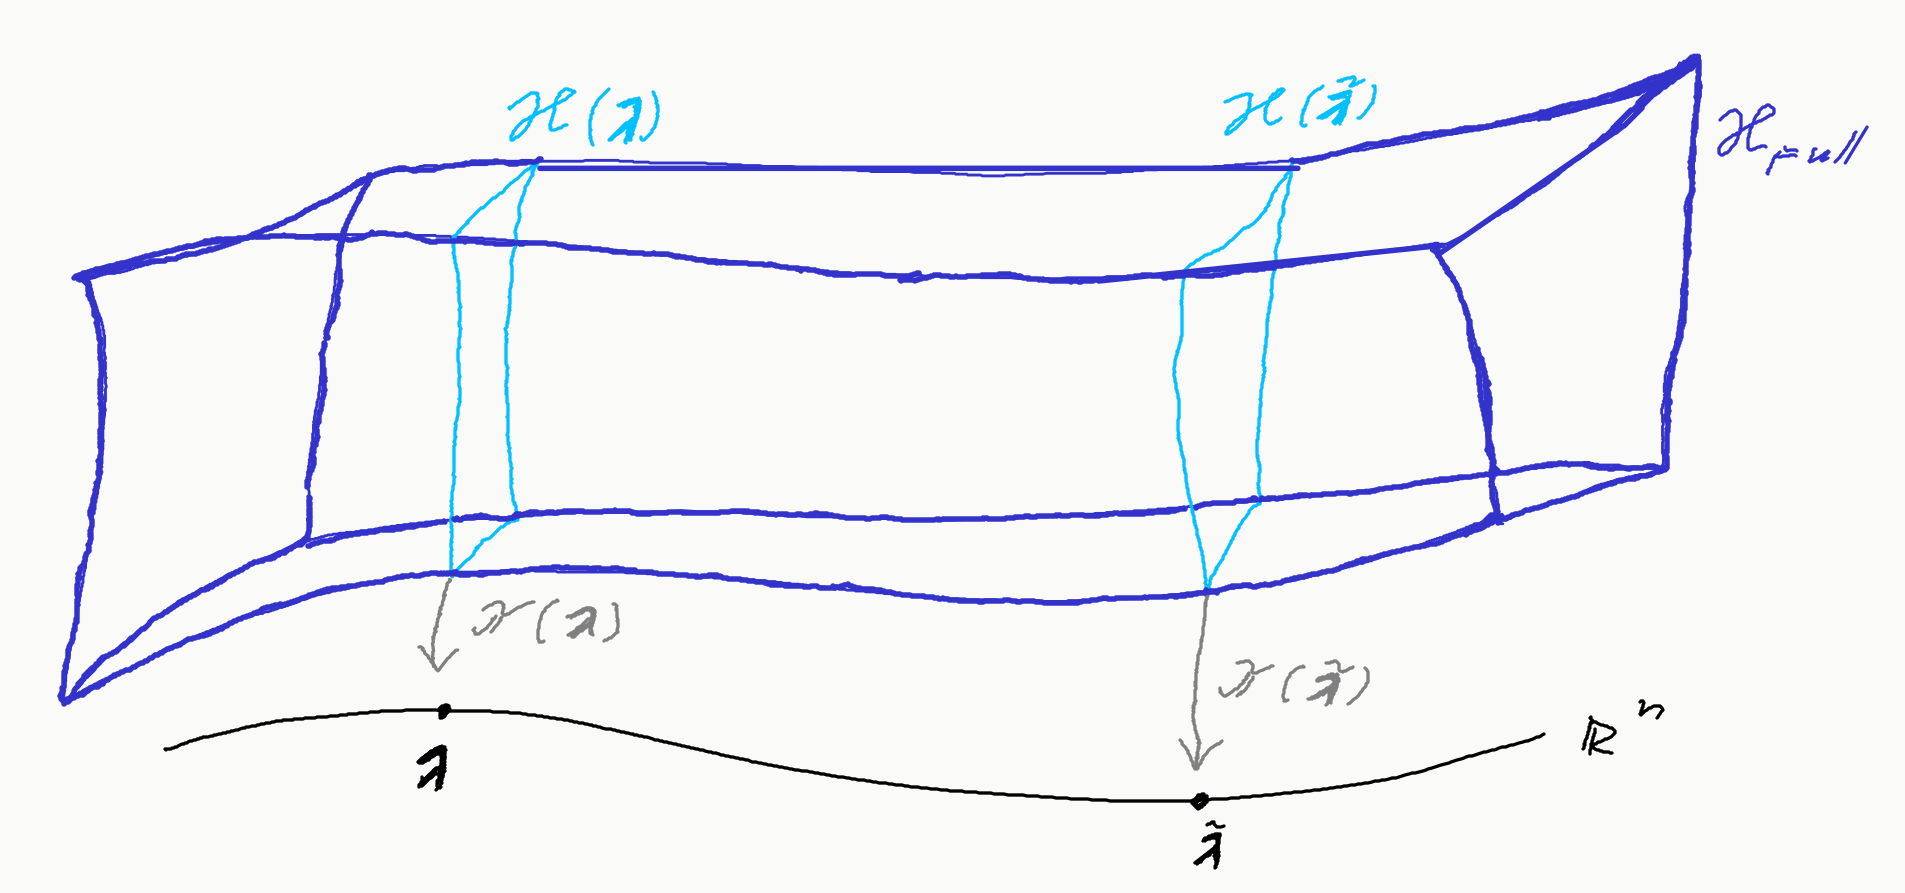
\includegraphics[width=\textwidth]{../img/manifold_basic.png}
\caption{Fiber bundle over $\R^n$ with Hilbert spaces $\H(\llambda)$ as individual fibers.}
    \label{fig:wholeBundle}
\end{figure}


Because we are interested only in discrete part of spectrum\footnote{Spectrum of the operator consists of discrete spectrum, calculable as eigenvalue problem, continuous and residual spectrum.}, it will further on be referred to only as \emph{spectrum}. 

The states of the system evolve according to the \Schrodinger equation
\begin{equation}
    i\hbar \d_t\kpsilt = \HH(\lambda)\kpsilt,
    \label{eq:schrodinger}
\end{equation}
which for eigenstates of instantaneous Hamiltonian reads as energy \Schrodinger equation
\begin{equation}
    \HH(\lambda)\ket{s(\lambda)}=E_s(\lambda)\ket{s(\lambda)}.
    \label{eq:energySchrodinger}
\end{equation}
For every $\H(\llambda)$ the first $k$ energies can be sorted from the lowest to create discrete set $\sigma(\HH(\llambda))\equiv\{E_0,\dots,E_k\}$. Clearly, there exists a bijection between all fibers $\H(\llambda)$, thus we can define \emph{section} $\mathrm{sec}_s$, mapping eigenstate corresponding to energy $E_s$ to base manifold 
$$\mathrm{sec}_s: \ket{o(\llambda)}\mapsto \mathcal{U}\subset \R^n,$$
which is also bijection\red{with an exception of singularities on ground state manifold?}. For $\forall s\in\{0,k\}$ we can create according to sec. \ref{sec:section} new \emph{energy manifolds}
$$\M_s\subset \M,$$
with special importance of the \emph{ground state manifold} $\M_0$, which will be used later on for adiabatic transports of ground states. Geometrical intuition is drawn on fig. \ref{fig:fullStructure}. Because those manifolds were created by sectioning, they are considered to be vector spaces in a geometrical sense. This was expected, because they contain quantum states, which themself are vectors.

\begin{figure}[h]
    \centering
    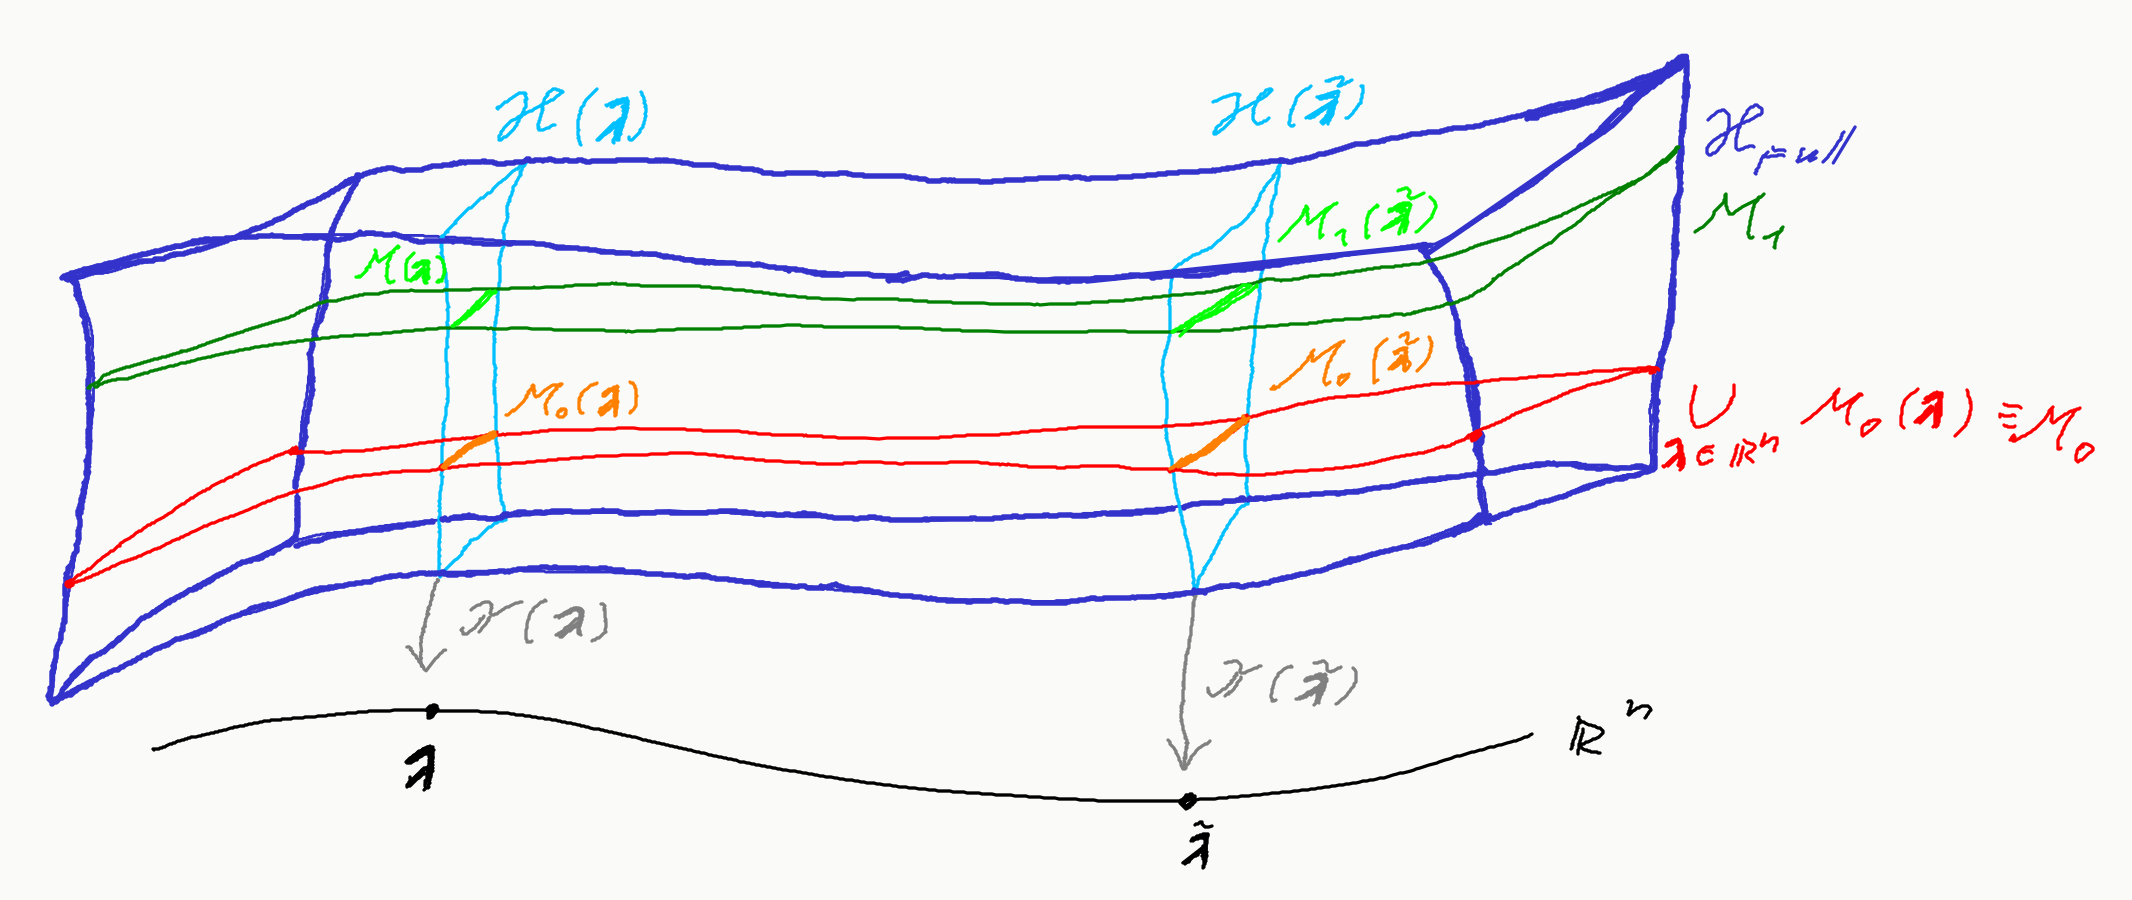
\includegraphics[width=\textwidth]{../img/manifold_full.png}
\caption{Geometrical intuition to transport on fiber manifold sections $\M_i$.}
    \label{fig:fullStructure}
\end{figure}




All Hilbert spaces above are considered to be spaces of \emph{bare states} $\H$. In quantum mechanics, physical observables are related to the \emph{space of rays}, defined as $\P\H\coloneqq \H/U(1)$, where elements of $U(1)$ are unitary transformations $e^{i\phi}$ for $\phi\in\R$ defining gauge symmetry between quantum states. This means that it is chosen the same for every vector. We cannot alter the phase of individual vectors. The geometrical intuition is drawn for any $\llambda$ on fig. \ref{fig:projectiveHilbertSpace}.
\begin{figure}[h]
    \centering
    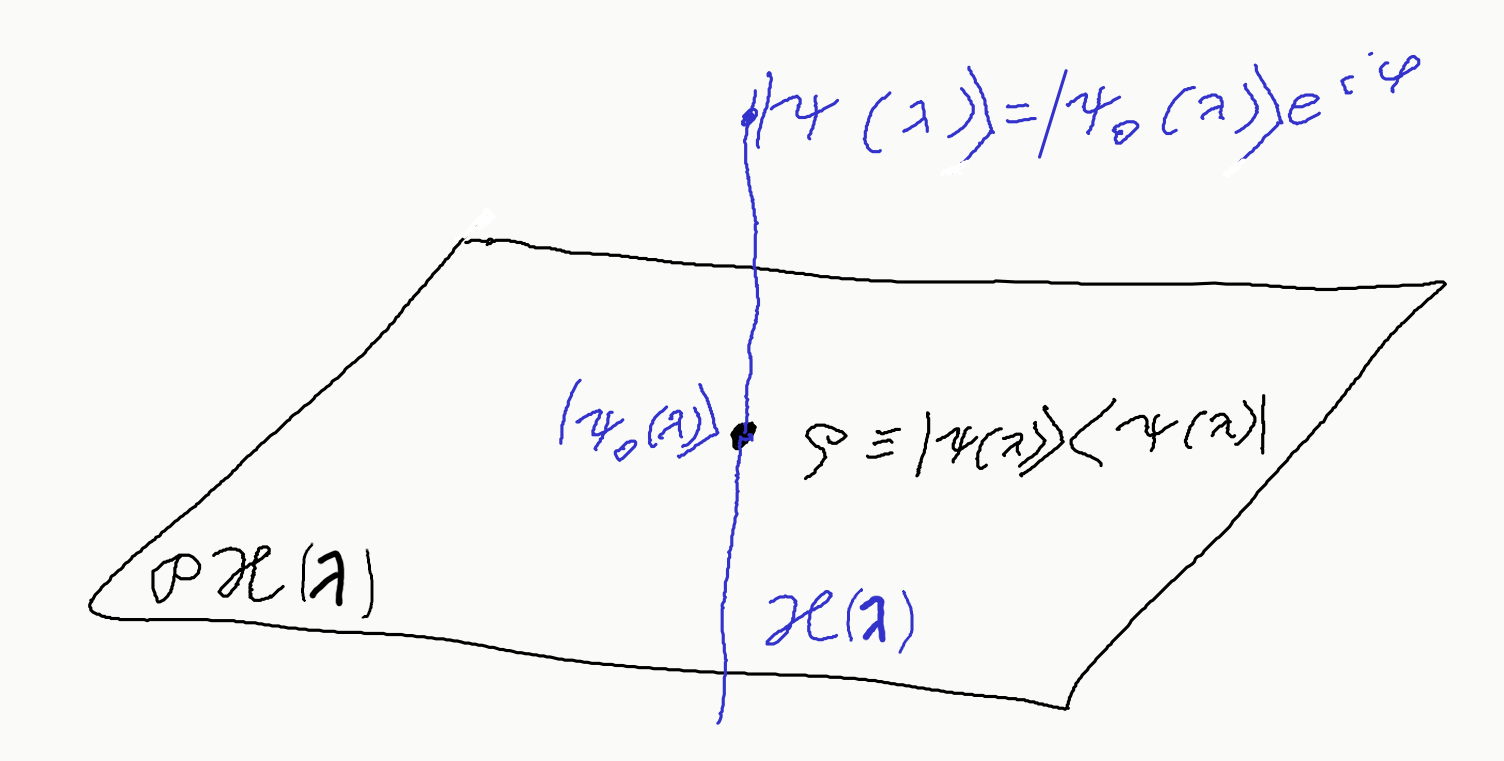
\includegraphics[width=0.8\textwidth]{../img/projectiveHilbertSpace.png}
\caption{Space of bare states and its projection to space of rays $\P\H(\llambda)\coloneqq \H(\llambda)/U(1)$.}
    \label{fig:projectiveHilbertSpace}
\end{figure}

This means, that energy manifolds $\M_s$, generated by bare states, are again of fiber structure, defined as
$$\left(\H,\P\H,\pi_{rays},\{e^{i\phi}\ket{\psi} \text{ for }\phi\in\R\}\right),$$
where $\pi_{rays}$ is just rule setting phase $\phi$ to zero. Because $\M_s$ are compact and connected, they are diffeomorphic to each other.








\section{Transporting states}
Let's now focus on decomposition of $\H_{full}$ to different state manifolds $\M_s$, as displayed on figure \ref{fig:manifoldCutIntuition}.

\begin{figure}[h]
    \centering
    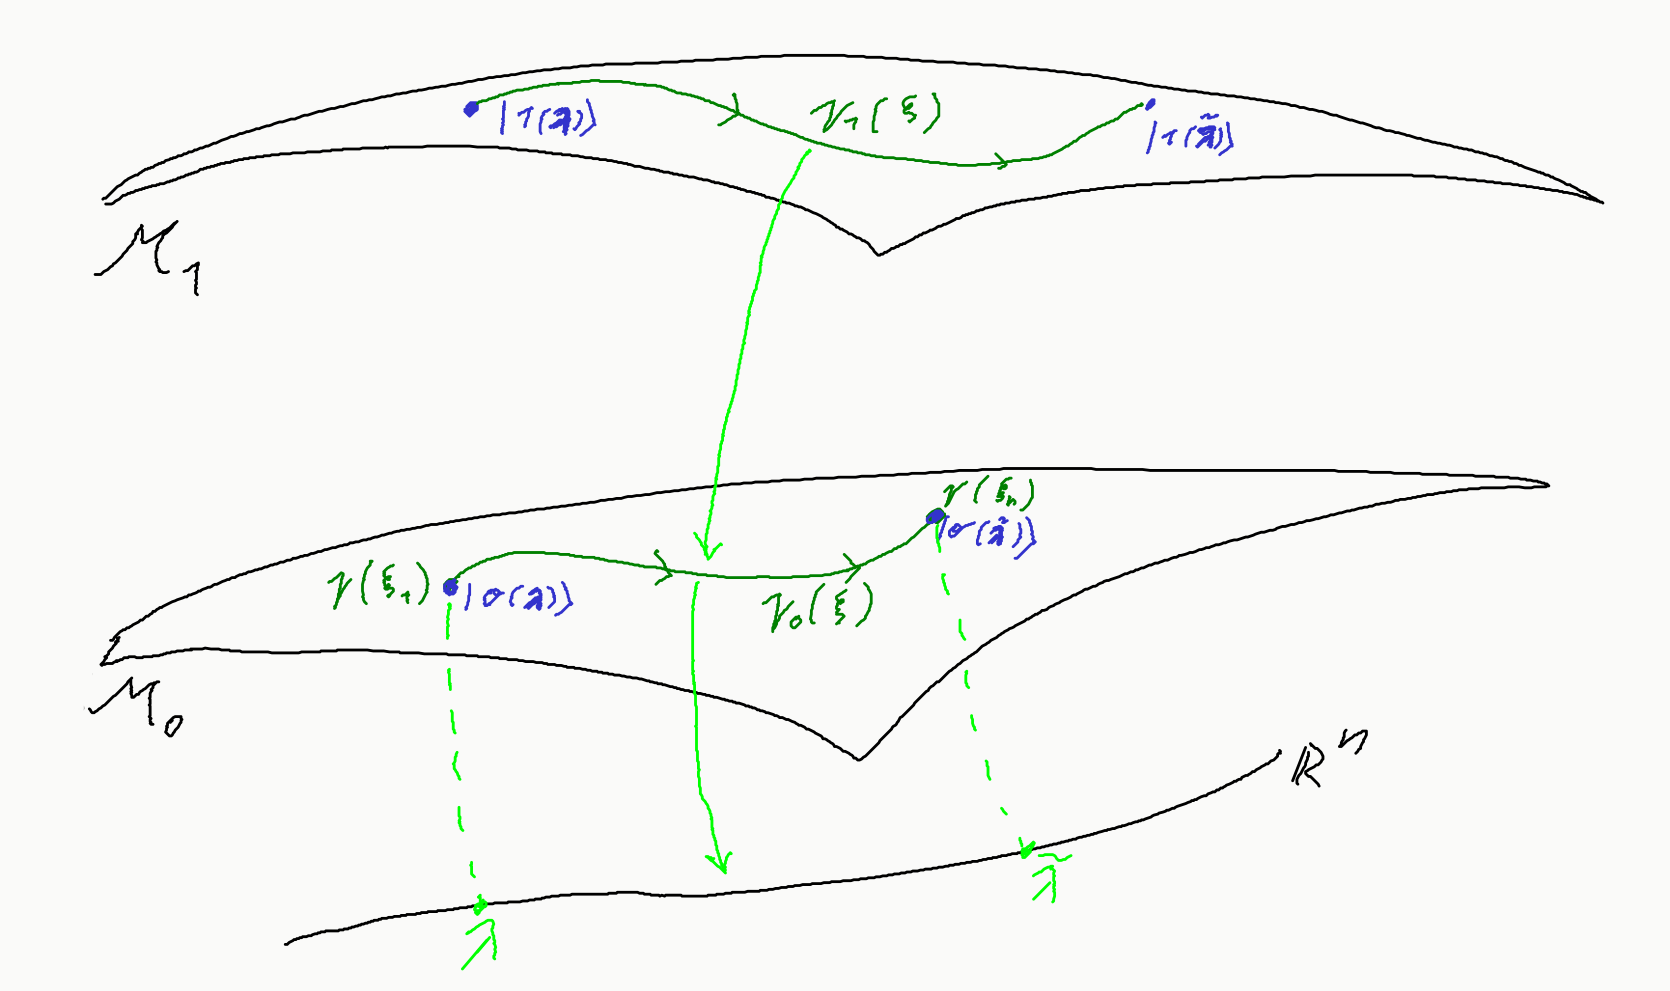
\includegraphics[width=\textwidth]{../img/manifoldCutIntuition.png}
\caption{Geometrical intuition to transport on fiber manifold sections $\M_s$.}
    \label{fig:manifoldCutIntuition}
\end{figure}

Changing state from eigenstate $\ket{s(\llambda)}$ to any pure state $\ket{\psi(\tilde\llambda)}$, during some time period, is unitary transformation and can be thought of as \emph{parallel transport on fiber bundle} between two vectors. Assuming the transport goes along curve $\{\gamma_s(\xi)|\xi\in[\xi_1,\xi_2]\subset \R\}\subset \M_s$ This can be written as
\begin{equation}
    \kpsit \equiv \Par_{\gamma_s}\ket{s(\lambda)} = \exp\left(-\frac{i}{\hbar}\int_0^tE_s(\tau)\d\tau)\right)\exp(i\gamma_s(\xi))\ket{s(\lambda)}.
    \label{eq:phasesOnManifold}
\end{equation}
The first exponential, the \emph{dynamical phase}, is well known solution to energy \Schrodinger equation \ref{eq:energySchrodinger} with $\llambda=const$ and depends only on time and energy of states during the transport. This dynamical phase changes the states only within the projective Hilbert space. The second exponential is called \emph{geometrical phase} and transports states within the full Hilbert space (changes their relative phase). This phase is generally non-integrable, meaning it cannot be written simply as $\gamma_s(\lambda)$ and for some closed curve on $\M$
\begin{equation}
    C=\{\llambda(\xi)|\xi\in[0,\Xi] \text{, such that }\llambda(0)=\llambda(\Xi)\}
\end{equation} 
we generally get $\Par_C \ket{\psi(\llambda)}\neq \ket{\psi(\llambda)}$. This property is sometimes more generally called an \emph{anholonomy} % and should be defined properly.
% \begin{definition}[Anholonomy]
%     Geometrical phenomenon, which causes some variable $V(\gamma(p))$ not to return to it's original value while varying it's parameter $p$ around some closed curve $\gamma(p)$. 
% \end{definition}
and geometric intuition can be seen on fig. \ref{fig:parallelTransportClosed}. This is where we are using the full Hilbert space, not only the projective Hilbert space.
\begin{figure}[h]
    \centering
    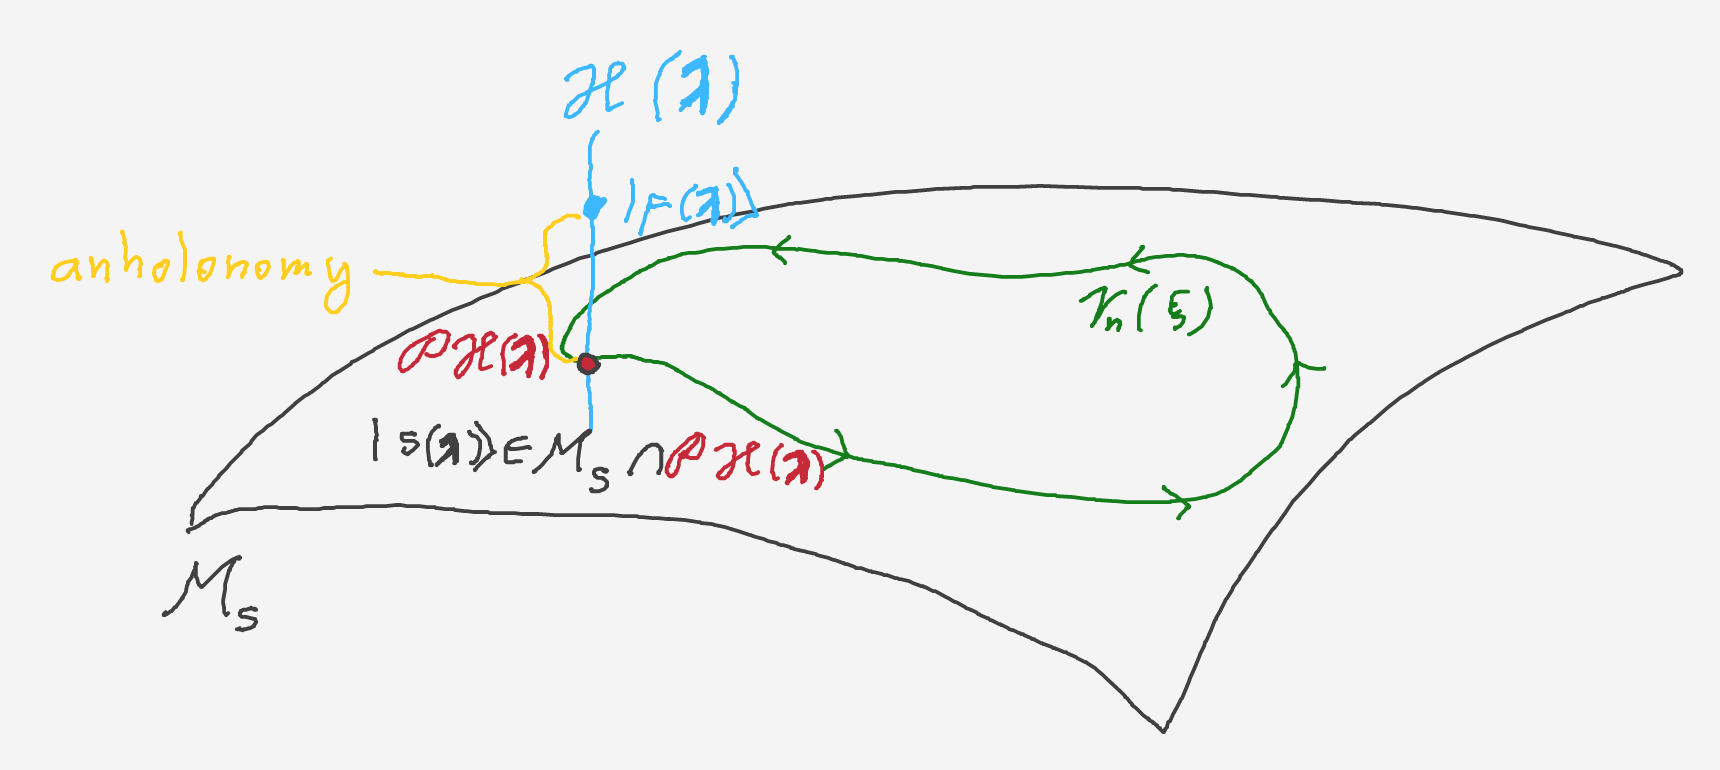
\includegraphics[width=0.8\textwidth]{../img/parallelTransportClosedCurve.png}
\caption{Parallel transporting around some closed curve $C$ with anholonomy drawn in yellow.}
    \label{fig:parallelTransportClosed}
\end{figure}

For quantum states, the anholonomy can be measured as a non-zero angle between $\ket{V}$ and $\Par_C\ket{V}$, meaning
\begin{equation}
    \braket{V|\Par_C|V}\neq 0.
\end{equation} 


Substituting general solution \ref{eq:phasesOnManifold} to eq. \ref{eq:schrodinger} yields (see \citep{berry1984}, \red{proof here})
\begin{equation}
    \d_t \gamma(\lambda)=i\braket{s(\lambda)|\partial_\mu s(\lambda)} \d_t \lambda^\mu(\lambda).
\end{equation}
Integrating this equation around some closed curve $C$ and assuming the dynamical phase to be zero, thus not exciting the system, we get
\begin{equation}
    \gamma_n(C)=i\oint_C\braket{s(\llambda)|\partial_\mu s(\llambda)}\d \lambda^\mu.
    \label{eq:gammaCoint}
\end{equation}
We see, that the geometric phase does not depend on energy or time, only on the sequence of Hamiltonians, which means it depends only on the path itself.




The problem of expressions above lies in $\partial_\llambda s(\llambda)$, which locally requires knowledge of single-valued basis $\{\ket{0},\dots, \ket{k}\}$. This can be avoided in 3-dimensions using Stokes's theorem for $S$ as the surface with boundary $\partial S=C$, for coordinate gradient $\nabla$
\begin{equation}
    \begin{split}
        \gamma_s(C) &= -\Im \iint_C \d S \cdot \nabla \times \braket{s(\llambda)|\nabla n(\llambda)}\\
         &= -\Im \iint_C \d S \cdot \braket{\nabla s(\llambda)|\times|\nabla s(\llambda)}\\
        &= -\Im \iint_C \d S \cdot \sum_{m\neq s} \braket{\nabla s(\llambda)|m(\llambda)}\times \braket{m(\llambda)|\nabla s(\llambda)}\\
        &= -\iint_C \d S \cdot V_s(\llambda)
            \label{eq:stokes}
    \end{split}
\end{equation}
for 
\begin{equation}
    V_s(\llambda) = \Im \frac{
            \braket{s(\llambda)\nabla_\llambda \HH(\llambda) |m(\llambda)}\times \braket{m(\llambda)|\nabla_\llambda \HH(\llambda)|s(\llambda)}    
             }{
(E_m(\llambda)-E_s(\llambda))^2
            }
\end{equation}
where the element of summation $m=s$ in third step of derivation is real, therefore has no influence on $\gamma_s$ and can be omitted. The last equivalence holds, because if we differentiate the \Schrodinger equation \ref{eq:energySchrodinger}, we get for any $\ket{s},\ket{m}\in \M$
\begin{equation}
    \begin{split}
        \nabla \HH\ket{s(\llambda)}+\HH \ket{\nabla s(\llambda)} &= E_s\ket{\nabla s(\llambda)}\\
        \braket{m(\llambda)|\nabla \HH|s(\llambda)}+\braket{m(\llambda)|E_m|\nabla s(\llambda)} &= \braket{m(\llambda)|\nabla \HH|s(\llambda)}\\
        \braket{m(\llambda)|\nabla s(\llambda)}&=
        \frac{\braket{m(\llambda)|\nabla \HH |s(\llambda)}}
        { E_m(\llambda)-E_s(\llambda)}, \qquad s\neq m,
    \end{split}
\end{equation}
where we used $\ket{\nabla s}\equiv\nabla \ket{ s}$. \textcolor{red}{or just use Feynman-Hellman equations, quantum geometric tensor pedagogical, page 5}
Comparing the first expression in eq. \ref{eq:stokes} with its last one and extending it to real numbers, we get
\begin{equation}
    V_s(\llambda)=\nabla\times\braket{s(\llambda)|\nabla m(\llambda)}, 
    \label{eq:vectorPotentialDef}  
\end{equation}
defining vector potential of $V_s(\llambda)$. In addition, it extends our definition from single valued basis to any solution of \ref{eq:energySchrodinger}, thus instead of ground state manifold, we can use any $\M_s$.

As was mentioned, the above procedure from eq. \ref{eq:gammaCoint} was performed only for three-dimensional space. Proper generalization to n-dimensional space would yield, see \citep{berry1984},
\begin{equation}
    \gamma_s(C) = -\iint_C (\bm\d S)^{\alpha\beta} \cdot\Im \frac{
            \overbrace{\braket{s(\llambda)\bm\d_\alpha \HH(\llambda) |m(\llambda)}}^{\in\TT_1\M}\wedge \overbrace{\braket{m(\llambda)|\bm\d_\beta\HH(\llambda)|s(\llambda)}}^{\in\TT_1\M}    
             }{
(E_m(\llambda)-E_s(\llambda))^2
             }.
\end{equation}






\section{Fidelity}


Generalization for any mixed state is for two density matrices $\sigma$, $\rho$ as $$f\coloneqq \left(\Tr \sqrt{\sqrt{\rho}\sigma\sqrt{\rho}}\right)$$





We can see it's physical meaning imagining \emph{quantum quench} (rapid change of some Hamiltonian parameters), in which case $f^2$ is the probability that system will remain in the new ground state. $1-f^2$ is therefore probability of exciting the system during this quench, 






\section{Metric and geometric tensor}
As a playground for this chapter, we will choose the projective ground state manifold $\P\M_0\equiv \cup_{\llambda\in\R^n} \{\ket{o(\llambda)}\}$, but it can be easily generalized to any energy state manifold $\P\M_s$. This means the geometrical phase will be neglected, because the states are the physical states from hte projective Hilbert space. From now on we will use natural units, so $\hbar=1$.
% Our first guess might be
% \begin{equation}
%     \d \tilde{s}^2 = \braket{i(\bm\llambda+\d\bm\llambda)|i(\bm\llambda+\d\bm\llambda)} = 1-2\Re{\braket{i(\bm\llambda+\bm\d\llambda)|i(\bm\llambda)}}.
% \end{equation}
% This is \emph{gauge dependent}, meaning that it depends on our choice of the wave phase, i.e. on observer. 

Let's first look at $\P\M_0$, which is needed to be \emph{gauge independent}. Gauge dependence in quantum mechanics means, that the change in phase factor $\phi$ of some state $\ket{o(\llambda)}\in \T_\llambda\M$ induces the change 
\begin{equation}
    \ket{o(\llambda)}\mapsto e^{i\phi(\llambda)} \ket{o(\llambda)} \implies \braket{o(\llambda)|\nabla o(\llambda)}\mapsto \braket{o(\llambda)|\nabla o(\llambda)} + i\nabla \phi(\llambda) 
\end{equation} 
For $\phi(\llambda)\in \mathcal C^2$ we see from eq. \ref{eq:vectorPotentialDef}, that gauge independent choice would be for infinitesimal change for example
\begin{equation}
    f=\braket{o(\bm\llambda+\delta\bm\llambda)|o(\bm\llambda)},
    \label{eq:fidelityDefinition}
\end{equation}
sometimes referred to as the \emph{fidelity of a ground state}. The meaning of fidelity as a probability transition between the states during some quench, leads to the definition of \emph{distance on $\M_0$}\footnote{$\d$ notation is in differential geometry assumed to be an exterior differential. On functions, it acts as $\d: \F\M\rightarrow \mathcal{T}_1\M$ and intuitively corresponds to total differential from functional analysis.}
\begin{equation}
    \d s^2 \equiv 1-f^2= 1-\left|\braket{o(\bm\llambda+\delta\bm\llambda)|o(\bm\llambda)}\right|^2.
    \label{eq:distanceOnM0}
\end{equation}
We can easily check, that the axioms of metric defined using distance (\red{this is why we dont use definition of metric from math intro}) as bilinear form $s$ between elements $\kpsi,\; \kphi\in \M_0$ are for \textcolor{red}{closed systems} satisfied:
\begin{itemize}
    \item identity of indiscernibles $s(\kpsi,e^{i\alpha}\kpsi) = 0 \Leftrightarrow \kpsi=\kphi$, $\alpha\in\R$,
    \item symmetry for any two states $\kpsi$, $\kphi$ is implied by $|\braket{\psi|\phi}|=|\braket{\phi|\psi}|$
    \item triangle inequality: $s(\kpsi,\ket{\psi_2}) <s(\kpsi,\kpsi_1) + s(\ket{\psi_1},\ket{\psi_2})$ for any $\ket{\psi_1}$.
\end{itemize}
Because $1-f^2>0$, the first term of Taylor expansion is zero, thus we have for a metric tensor
\begin{equation}
    \d s^2 = g_{\mu\nu}\d \lambda^\mu \d\lambda^\nu+\O(\lambda^3).
    \label{eq:metricTensorDef}
\end{equation} 

Let's define the metric on the space of states $\M_0$ and then see, how it corresponds to fidelity. This metric is called the \emph{Geometric tensor}, and can be expressed as 
\begin{equation}
    \chi_{\mu\nu}\coloneqq \braket{\partial_\mu o|\partial_\nu o}_c \equiv \braket{\partial_\mu o|\partial_\nu o} - \braket{\partial_\mu o|o}\braket{o|\partial_\nu o},
    \label{eq:geometricTensor}
\end{equation}
where shortened notation $\partial_\nu\coloneqq\pder{}{\lambda^\nu}$ was used. 

%taylor is wrong
% \begin{proof}[Proof for Geometric tensor expression] In one-dimensional case we get from eq. \ref{eq:fidelityDefinition} using Taylor expansion and shortened notation $o\coloneqq o(\lambda)$
%     \begin{equation}
%         f=1+\braket{\partial_\lambda o|o}\delta\lambda-\frac{1}{2}\braket{\partial_\lambda^2 o|o}\delta\lambda^2+\mathcal{O}(\lambda^3),
%     \end{equation}
%     which plugged into eq. \ref{eq:distanceOnM0} gives
%     \begin{equation}
%         \begin{split}
%             \d s^2&=1-\bar{f}f=\left[-\braket{o|\partial_\lambda o}\braket{\partial_\lambda o|o}+\frac{1}{2}\braket{\partial_\lambda^2 o|o}+\frac{1}{2}\braket{o|\partial_\lambda^2 o}\right]\delta \lambda^2.
%         \end{split}
%     \end{equation}
%     Generalizing for $\lambda\in \R^n$, we get\footnote{assuming Hermiticity of the derivative operator everywhere on the ground state manifold}
%     \begin{equation}
%         \d s^2=\left[-\braket{o|\partial_\mu o}\braket{\partial_\nu o|o}+\underbrace{\frac{1}{2}\braket{o|\partial_\mu \partial_\nu|o}+\frac{1}{2}\braket{o|\partial_\nu \partial_\mu| o}}_{\Re\braket{\partial_mu o|\partial_\nu o}}\right]\delta \lambda^\mu\delta \lambda^\nu.
%     \end{equation}
%     Because only symmetric part contributes in the sum in eq. \ref{eq:metricTensorDef}, this proves symmetric part of equation \ref{eq:geometricTensor} and shows, that some more general tensor (\emph{geometric tensor}) exists.
% \end{proof}

It is practical to decompose it to the geometric tensor
\begin{equation}
    \chi_{\mu\nu} \equiv g_{\mu\nu} - i\frac{1}{2} \nu_{\mu\nu},
\end{equation}
where the \emph{Fubini-Study tensor}\footnote{In some literature, this is called Geometric tensor}, as it's called, is metric on $\P\M_0$ and can be expressed as
\begin{equation}
    g_{\mu\nu} = \frac{\chi_{\mu\nu}+\chi_{\nu\mu}}{2} = \Re\braket{\partial_\mu o|\partial_\nu o}_c = \Re \sum_{o\neq j}\frac{\braket{o|\pder{\H}{\lambda^\mu}|j}\braket{j|\pder{\H}{\lambda^\nu}|o}}{(E_o-E_j)^2},
    \label{eq:metrictensorREdefinition}
\end{equation}
and the \emph{curvature tensor} a.k.a. \emph{Berry curvature} is
\begin{equation}
        \nu_{\mu\nu} = i(\chi_{\mu\nu}-\chi_{\nu\mu})= \Im\braket{o|[\curlyleftarrow{\partial}_\nu,\partial_\mu]|o}_c = -2 \Im \sum_{o\neq j}\frac{\braket{o|\pder{\H}{\lambda^\mu}|j}\braket{j|\pder{\H}{\lambda^\nu}|o}}{(E_o-E_j)^2},
    \label{eq:geom.tensorREdefinition}
\end{equation}
where $\curlyleftarrow{\partial}_\nu$ affects the covector on the left.


\subsection{Derivation of the geometric tensor}
\label{sec:derivationOfGeometricTensor}
To prove the correspondence of geometric tensor, described by eq. \ref{eq:geometricTensor}, to distance on $\M_0$, see eq. \ref{eq:distanceOnM0}, we start with eigenstate $\ket{o(\llambda)}\in \M_0\cap \H(\llambda)$. Changing parameters $\llambda$ to $\llambda+\delta \llambda$ results in Hamiltonian $\HH_f$ with eigenstates $\ket{s(\llambda+\delta \llambda)}\in \M_s\cap\H(\llambda+\delta \llambda)$, meaning it can be excited. Probability amplitude of going to such state is
\begin{equation}
    \begin{split}
        a_s&=\braket{s(\llambda+\delta\llambda)|o(\llambda)}\approx \delta\lambda^\mu\braket{\partial_\mu s(\llambda)|o(\llambda)} \\
        &= -\delta\lambda^\mu\braket{s(\llambda)|\partial_\mu|o(\llambda)}.
    \end{split}
\end{equation}

If we introduce the \emph{gauge potential}, aka \emph{calibration potential}, as\footnote{In SI units, the gauge potential is $\AA_\mu\equiv i\hbar\partial_{\mu}$}
\begin{equation}
    \AA_\mu\equiv i\partial_{\mu},
\end{equation}
the probability amplitude can be expressed as
\begin{equation}
   a=i\braket{s(\llambda)|\AA_\mu |o(\llambda)}\delta\lambda^\mu,
   \label{eq:probabilityOfTransitionIsGauge}
\end{equation}
which has meaning of matrix elements of the gauge potential. Probability of the excitation i.e. transition to any state $s>0$ from ground state is then (omitting the $\llambda$ dependence in notation)
\begin{equation}
    \begin{split}
        \sum_{s\neq 0}|a_s|^2&=  \sum_{s\neq 0} \delta \lambda^\mu \delta \lambda^\nu\braket{o|\AA_\mu|s}\braket{s|\AA_\nu|o}+\O(|\delta \lambda^3|) \\
        &= \delta \lambda^\mu \delta \lambda^\nu\braket{o|\AA_\mu \AA_\nu|o}_c\eqqcolon \delta \lambda^\mu \delta \lambda^\nu\chi_{\mu\nu}+\O(|\delta \lambda^3|),
    \end{split}
\end{equation}
where last term defines the geometric tensor.











\section{Berry phase and curvature}
Let's consider only the ground state manifold, because it will be used later on. Thought every step can be easily generalized to any state manifold $\M_s$.

On the ground state manifold $\M_0\equiv \cup_{\phi\in\R}\cup_{\llambda\in\R^n} e^{i\phi}\{\ket{o(\llambda)}\}$, the \emph{Berry connection} is defined as
\begin{equation}
    A_\mu(\llambda)\equiv \braket{o(\llambda)|\AA_\mu|o(\llambda)}\coloneqq -i\hbar \braket{o(\llambda)|\partial_\mu|o(\llambda)},
    \label{eq:berryConnection}
\end{equation}
which uses the decomposition of $\llambda$ to some basis, thus it empowers us to take derivatives in any direction in the base manifold $\R^n$ and thus the geometric tensor can be written as
\begin{equation}
    \chi_{\mu\nu}(\llambda) = \partial_\mu A_\nu(\llambda)-\partial_\nu A_\mu(\llambda)
\end{equation}
and the \emph{Berry phase}\footnote{
    The reasonability of this definition can be seen, if we assume the ground state of a free particle
        $\braket{\bm{x}|i(\llambda)}=i(\bm{x},\llambda)= |i(\bm{x})|e^{i\phi(\llambda)}$,
    then the Berry connection is
    \begin{equation}
        A_\mu=-\int \d \bm{x}|i(\bm{x},\llambda)|^2\partial_\mu \phi(\llambda) = -\partial_\mu \phi(\llambda)
    \end{equation} 
    and Berry phase
    \begin{equation}
        \phi_B=\oint_\mathcal{C} \partial_\mu \phi \d \lambda^\mu,
    \end{equation}
    which represents total phase accumulated by the wave function. It is really the analogy for Berry phase in classical mechanics, which for example in the case Foucault pendulum on one trip around the Sun makes $\phi_B=2\pi$
}
as the integral of the Berry connection along some closed curve $\mathcal{C}$
\begin{equation}
    \phi_B\equiv-\oint_\mathcal{C} A_\mu(\llambda)\d \lambda^\mu=\int_\mathcal{S} \chi_{\mu\nu}(\llambda)\d \lambda^\mu \wedge \d\lambda^\nu,
\end{equation}
where we used the Stokes theorem for some area $\mathcal{S}$ with boundary $\partial\mathcal{S}=\mathcal{C}$.

Berry phase is usually zero, except for the cases, when the curve goes around some geometric tensor singularity, meaning $\mathrm{Ind}_a \gamma(\lambda)>0$. Those singularities appear in the system due to energy spectrum degeneracies, in the case of ground state manifold, when $E_1-E_0=0$. Those points are called \emph{diabolic}, because of their shape in the $(\lambda,\chi)$ parameter space.\footnote{https://en.wikipedia.org/wiki/Diabolo}












\section{General fidelity driving}

\subsection{APT}
From \cite{Rigolin2008}.
One important thing to bare in mind is \emph{locality of variables}. Let's call variable $V(s)$ \emph{\bluee{local}} if it depends only on infinitesimal sirrounding of $s$. These variables will be in shades of blue and non-local variables in shades of red.

The power series will be derived using a small parameter $v=1/T$. Starting again with
\begin{equation}
    \red{\ket{\Psi(s)}}=\sum_{p=0}^\infty v^p \red{\ket{\Psi^{(p)}(s)}},
    \label{eq:mainSeries}
\end{equation}

for 
\begin{equation}
    \red{\ket{\Psi^{(p)}(s)}}=\sum_{n=0} e^{-\frac{i}{v} \reddd{\omega_n(s)}}e^{i\reddd{\gamma_n(s)}}\redd{b_n^{(p)}(s)}\bluee{\ket{n(s)}}.
\end{equation}
Here the
\begin{align}
    \reddd{\omega_n(s)} &\coloneqq \frac{1}{\hbar}\int_0^s \bluee{E_n(s')}\d s'\\
    \reddd{\gamma_n(s)} &\coloneqq i\int_0^s \bluee{\braket{n(s')|\frac{\d}{\d s'}n(s')}}\d s' \equiv i\int_0^s \bluee{M_{nn}(s')}\d s'
    \label{eq:gammadef}
\end{align}
are so-called \redd{dynamical} resp. \redd{Berry (geometric) phase} and $\bluee{\ket{n(s)}}$ are solution to
\begin{equation}
    \bluee{\HH(s)\ket{n(s)}}=\bluee{E_n(s) \ket{n(s)}}.
\end{equation}
Variables $\reddd{\omega_n(s)}$ and $\reddd{\gamma_n(s)}$ are defined using integration over the whole protocol, therefore there are \emph{\red{non-local variables}}.
The problem now lies in determining $\redd{b_n^{(p)}(s)}$, which is also \red{nonlocal}. Because it depends on its relative \reddd{geometric} and \reddd{dynamical phase} to other \bluee{energy levels}, lets write it as a series
\begin{equation}
    \redd{b_n^{(p)}(s)}=\sum_{m=0} e^{\frac{i}{v}\reddd{\omega_{nm}(s)}}e^{-i\reddd{\gamma_{nm}(s)}}\blue{b_{nm}^{(p)}(s)},
\end{equation}
where $\reddd{\omega_{nm}} \coloneqq \reddd{\omega_m}-\reddd{\omega_n}$, $\reddd{\gamma_{nm}} \coloneqq \reddd{\gamma_m}-\reddd{\gamma_n}$.  The reason for \blue{locality} of $\blue{b_{nm}^{(p)}(s)}$ will be clear soon.

Inserting all to original series \ref{eq:mainSeries}, we get
\begin{equation}
    \red{\ket{\Psi(s)}}=\sum_{n,m=0}\sum_{p=0}^\infty v^p e^{-\frac{i}{v}\reddd{\omega_m(s)}}e^{i\reddd{\gamma_m(s)}}\redd{b_{nm}^{(p)}(s)}\bluee{\ket{n(s)}}.
    \label{eq:solve0}
\end{equation}

Because the initial state is eigenstate, we get initial conditions $\blue{b_{nm}^{(0)}(s)=0}$. In addition, one can rewrite equation \ref{eq:solve0} to the iteratively solvable form
\begin{equation}
    \frac{i}{\hbar}\bluee{\Delta_{nm}(s)}\blue{b_{nm}^{(p+1)}(s)}+\blue{\dot b_{nm}^{(p)}(s)}+\bluee{W_{nm}(s)} \blue{b_{nm}^{(p)}(s)}+\sum_{k=0,k\neq n}\bluee{M_{nk}(s)}\bluee{b_{km}^{(p)}(s)}=0,
    \label{eq:bSolution}
\end{equation}
for $\bluee{\Delta_nm(s)}\coloneqq \bluee{E_m-E_n}$, $\bluee{W_{nm}(s)}\coloneqq \bluee{M_{nn}(s)}-\bluee{M_{mm}(s)}$, where $\bluee{M_{mn}}$ is defined in Eq. \ref{eq:gammadef}. We can see that $\blue{b_{mn}^{(p)}}$, as a solution to Eq. \ref{eq:bSolution},\textbf{ only depends on difference between energy levels, eigenstates during the path and their directional derivatives. Not on the path itself}. All of those are easily obtained, once the driving path is prescribed.

    










\section{How to advantageously drive the system}

\subsection{Adiabatic driving}
Adiabatic transformation is such a transformation from $\M$ to $\M$, which does not excite the system, meaning the fidelity $f=1$. Generally it can be achieved by two ways -- infinitely slow transformation of states, or adding some \emph{counter-diabatic elements} to the Hamiltonian to counter the excitation.


In this chapter, we will be dealing with the system described by the finite-dimensional Hamiltonian $\HH(\llambda)$ which drives the system according to \Schrodinger equation from some initial state $\ket{s(\llambda}$ to $\ket{s(\tilde\llambda)}$ along the path $\gamma(\lambda)$. Before going throw the details of adiabatic transformations, let's define its meaning properly.

\begin{definition}[Adibaticity]
    Slow change of parameters driving Hamiltonian in a sense, that it does not excite the system and allows the system to return to the same energetic state after circulation around any closed path on the manifold with fidelity $f=1$.
\end{definition}


\subsubsection{Slow transports}
\citep{kolodrubez}[chap. 2.3]
As was mentioned in the introduction of this chapter, one way to change the system parameters without exciting it is to change the driving parameter slowly enough. The meaning of the word "slow" clears up next theorem.
\begin{thm}[Adiabatic theorem]
    \label{adiabaticTheorem}
    For Hamiltonian $\HH$ varying in the time range $T$, the solution of the Schrödinger equation 
    $$\HH(\lambda)\ket{\psi_n(\lambda)} = E_n(\lambda)\ket{\psi_n(\lambda)}$$
    with initial condition in x-representation $\braket{x|\psi(t=0}=\psi_n(x,0)$ can be approximated as
    \begin{equation}
      ||\psi(\lambda) - \psi_{ad}(\lambda)||\approx o\left(\frac{1}{T}\right)
    \end{equation}
    for \emph{adiabatic state}
    \begin{equation}
        \ket{\psi_{ad}}= e^{\theta_n(\lambda)}e^{\gamma_n(\lambda)}\ket{\psi(\lambda)},
    \end{equation}
    where we define \emph{nongeometrical phase} induced by energy transitions,
    $$\theta_n(\lambda)\equiv -\frac{1}{\hbar}\int_0^t E_n(\tau)\d \tau$$
    and \emph{geometrical phase}, also called \emph{Berry phase}
        $$\gamma_n(\lambda)\equiv \int_0^t \underbrace{i\braket{\psi_n(\tau)|\partial_t\psi_n(\tau)}}_{\nu_n(\tau)} \d \tau .$$
\end{thm}
\begin{myproof}
    \textcolor{blue}{TBD (is on wikipedia :)} )
\end{myproof}
Assume differentiable and non-singular Hamiltonian $\HH(\llambda)$ with degenerate basis $\{\ket{m,\llambda}\}_m$ called the \emph{adiabatic basis}. This is generally the family of adiabatically connected eigenstates\footnote{In the case of energy level crossing, the eigenstates are not unified, because transition between them is not adiabatical.} The transition amplitude between states for adiabatic change is
\begin{equation}
    0=\bra{m(\llambda)}\HH\ket{n(\tilde\llambda)} \quad \text{for }n\neq m, \forall \llambda,\forall \tilde \llambda.
\end{equation}
This can be driven along some curve $\gamma(\lambda)$, i.e. differentiated by $\partial_t$:
\begin{equation}
    \begin{split}
        0&=\bra{\partial_t m(\llambda)}\HH(\tilde \llambda)\ket{n(\tilde\llambda)}+ \bra{m(\llambda)}\overbrace{\partial_t\HH(\tilde \llambda)}^{\approx \partial_t\HH(\llambda)}\ket{n(\tilde\llambda)}+ \bra{m(\llambda)}\HH(\tilde \llambda)\ket{\partial_t n(\tilde \llambda)}\\
        &=E_n(\lambda)\braket{\partial_t m(\llambda)|n(\tilde \llambda)} + E_m(\lambda)\braket{m(\llambda)|\partial_t n(\tilde \llambda)}+ \bra{m(\llambda)}\partial_t \HH(\tilde\llambda)\ket{n(\tilde \llambda)}\\
        &= (E_m(\lambda)-E_n(\lambda))\underbrace{\braket{m|\partial_t (\tilde \llambda)}}_{-\frac{i}{\hbar}\bra{m}\AA_t\ket{n(\tilde \llambda)}} + \braket{m|\partial_t\HH|n(\tilde \llambda)}.
    \end{split}
\end{equation}

This can be rewritten in matrix form as
\begin{equation}
    i\hbar\partial_t\HH=[\AA_t,\HH]-i\hbar \hat{M}_t\qquad \text{for } \hat{M}_t\equiv -\sum_n\pder{E_n(\lambda)}{t}\ket{n(\lambda)}\bra{n(\lambda)}.
\end{equation}
$\hat{M}$ is diagonal in energetic basis and its elements has meaning of \emph{generalized force}. We can easily see that $[\HH,\hat{M}]=0$, implying
\begin{equation}
    [\HH,i\hbar\partial_t\HH-[\AA_t,\HH]]=0.
    \label{eq:komutation}
\end{equation}
This can be used as the definition for \emph{counter-diabatic potential} $\AA_t$, because it was obtained from only one assumption -- adiabaticity. The strength of this equation lies in fact, that it finds counter-diabatic potential without the need of Hamiltonian diagonalization.




\subsection{Counterdiabatic driving}
\subsubsection{Gauge potentials}
In section \ref{sec:derivationOfGeometricTensor} we introduced the gauge potential without proving its gauge meaning, but only stating its correspondence to transition probability, see eq. \ref{eq:probabilityOfTransitionIsGauge}.
\emph{Gauge transformations}, in classical mechanics called \emph{canonical}, can be defined such, that they \emph{preserve Lagrangian of the system under local transformations from some Lie group}. This implies, that gauge transformed Hamiltonian $\HH(\llambda)$ and $\HH(\llambda+\d \llambda)$ commutes with its canonically transformed version\footnote{This can be easily reformulated to the world of classical physics, where the commutator is replaced by Poisson bracket.} 
 \begin{equation}
     [\HH(\llambda),\HH(\llambda+\delta \llambda)]=0.
 \end{equation}

 To understand the meaning of gauge symmetries, let's first consider classical system and then move to quantum mechanics.




\subsubsection{Classical gauge potential}
In the Hamiltonian classical mechanics, we assume the manifold $\M$ as subset of the phase space defined by Hamiltonian $H=H(p_i,q_i)$, where momentum $p_i$ and position $q_i$ are assumed to form the orthogonal basis of the phase space
\begin{equation}
    \{q^i,p_j\}=\delta^i_j,
    \label{eq:canonicalCommutationDelta}
\end{equation}
which also defines \emph{calibrational freedom} in their choice. \emph{Canonical transformations} then by definition preserve this formula. Using the \emph{Poisson bracket}, defined as
\begin{equation}
    \{A,B\}\coloneqq \pder{A}{q^j}\pder{B}{p_j}-\pder{B}{q^j}\pder{A}{p_j},
\end{equation}
we will examine continuous canonical transformations generated by gauge potential $\A_\lambda$
\begin{align}
        q^j(\lambda+\delta\lambda)&=q^j(\lambda)-\pder{\A_\lambda(\bm{p},\bm{q})}{p_j}\delta\lambda \;\Rightarrow\; \pder{q^j}{\lambda}=-\pder{\A_\lambda}{p_j}=\{\A_\lambda,q^j\}
        \label{eq:gaugeAsGeneratorOfMotion1}\\
        p_j(\lambda+\delta\lambda)&=p_j(\lambda)-\pder{\A_\lambda(\bm{p},\bm{q})}{q^j}\delta\lambda \;\Rightarrow\; \pder{p_j}{\lambda}=-\pder{\A_\lambda}{q^j}=\{\A_\lambda,p_j\}.
        \label{eq:gaugeAsGeneratorOfMotion2}
\end{align}
Substituting this to relations of orthogonality \ref{eq:canonicalCommutationDelta}, we get
\begin{equation}
    \{q^j(\lambda+\delta\lambda),p_j(\lambda+\delta\lambda)\}=\delta^i_j + \mathcal{O}(\delta\lambda^2).
\end{equation}
 
If $\lambda$ is time parameter and $\A_t=-H$, equations \ref{eq:gaugeAsGeneratorOfMotion1},\ref{eq:gaugeAsGeneratorOfMotion2} are identical to the Hamilton equations
\begin{equation}
\begin{split}
    \dot{q}^j&=-\{H,q^j\} = \pder{H}{p_j}\\
    \dot{p}_j&=-\{H,p_j\} = -\pder{H}{q^j}.
\end{split}
\end{equation}
Because the Hamiltonian is generator of the movement in the phase space $(\bm{q},\bm{p})$, we can interpret $\A_t$ as the generators of the movement on $\M$. Other specific choice might be $\lambda=X^i$, which gives us the momentum components $\A_{X^i}=p_i$.

Generally every gauge symmetry is generated by its gauge potential and corresponds to some conserved property, as theorem of Emma Nöether states.





\subsubsection{Quantum gauge potential}
\citep{kolodrubez}[chap. 2.2]
The role of Poison brackets in quantum mechanics is taken by commutators, canonical transformations are called \emph{unitary transformations} and calibration freedom is hidden in the choice of basis. Now let's find some special basis transformations $\U$ between initial system $S$ and the transformed $\tilde{S}$. Both of them describe the system with Hamiltonian $\HH(\llambda)$ with eigenstates $\ket{n(\llambda)}$ and eigenstate manifolds $\M_n\equiv \cup_\llambda \{\ket{n(\llambda)}\}$. 

From fiber structure goes\footnote{especially from the fact, that all spaces $\HH(\llambda)$ are isomorphic to each other}, that any state of $\HH(\llambda)$ for $\forall \llambda\in U\subset \R^n$ can be decomposed as
    \begin{equation}
    \ket{\psi(\llambda)}\equiv \sum_n \psi_n(\llambda)\ket{n}
\end{equation}    
for some coordinate independent basis $\{\ket{n}\}_n$.
Then there exist unitary transformation
\begin{equation}
    \U(\llambda): \tilde S\rightarrow S,\quad \U(\llambda)\ket{m(\llambda)}=\ket{n}.
    \label{eq:transformationU}
\end{equation}
where scalar parameter $t$ is assumed to be changing along the path $\gamma(t)$, corresponding to situation on fig. \ref{fig:manifoldCutIntuition}. This satisfies
\begin{equation}
    i\hbar \partial_t \U(t)=\HH(t)\U(t)
    \label{eq:schrodingerForU}
\end{equation}
for $\HH$ the full Hamiltonian of the system and any point on $\tilde\gamma(t)$, along which the partial derivative is taken.


The wave function $\kpsi$ in $S$ can be decomposed using Schmidt decomposition\footnote{The Schmidt decomposition can be performed in finite dimension, or if the Hamiltonian is compact, which is not automatic in quantum mechanics. What's more, the Hamiltonian is usually not even bounded. Anyway, for simple systems with bounded energy we can assume so.}
\begin{equation}
    \ket{\psi(\llambda)} = \sum_{m,n}\psi_n(\llambda) \ket{m(\llambda)}\overbrace{\braket{m(\llambda)|n}}^{U_{mn}(\llambda)} =\sum_m \overbrace{\tilde{\psi}_m(\llambda)}^{\braket{m(\llambda)|\psi_n|n}}\ket{m(\llambda)},
\end{equation}
where $U_{mn}(\llambda)$ are matrix elements of unitary transformation $\U(\llambda)$. In this work, we will be interested only in the gauge transformations preserving energy of the system.





\subsubsection{Adiabatic gauge potential}

Adiabatic gauge potentials, sometimes just \emph{adiabatic potentials}, are generators of unitary transformations, so we can define them analogically to the classical case
\begin{equation}
    i\hbar\partial_\lambda \ket{\tilde{\psi}(\llambda)} = i\hbar \partial_\lambda\left(\U^+(\llambda)\ket{\psi} \right)= \underbrace{i\hbar\left(\partial_\lambda \U^+(\llambda)\right)\U(\llambda)}_{-\tilde{\AA_\lambda}}\ket{\tilde{\psi}(\llambda)}.
\end{equation}
The adiabatic potential $\tilde{\AA_\lambda}$ can be transformed to non-tilde system as
\begin{equation}
    \begin{split}
        \AA_\lambda&=\U(\llambda)\tilde{\AA_\lambda}\U^+(\llambda) = -i\hbar\U(\llambda)\big(\partial_\lambda \U^+(\llambda)\big) =\\
        &= -i\hbar\partial_\lambda\big(\underbrace{U^+(\llambda)U(\llambda)}_{\mathds{1}}\big)-\big(\partial_\lambda U(\llambda)\big)U^+(\llambda) \big) =i\hbar \big(\partial_\lambda U(\llambda\big)U^+(\llambda).
    \end{split}
\end{equation}
From this we get the equations for adiabatic potential in two systems
\begin{align}
    \AA_\lambda&=i\hbar \big(\partial_\lambda U(\llambda)\big)U^+(\llambda)
    \label{eq:adiabaticPotential}\\
    \tilde{\AA_\lambda} &= -i\hbar\left(\partial_\lambda \U^+(\llambda)\right)\U(\llambda)
    \label{eq:adiabaticPotentialTilde}
\end{align}
which can be shown to be Hermitian
\begin{equation}
     \tilde{\AA_\lambda}^+=i\hbar U(\llambda)^+\big(\partial_\lambda\U(\llambda)\big)=-i\hbar\big(\partial_\lambda\U(\llambda)^+\big)\U(\llambda) = \tilde{\AA_\lambda},
     \label{eq:counterdiabaticPotentialTwoSystems}
\end{equation}
analogically for non-tilde potential.
Using the eigenbasis of $\HH$, the matrix elements are
\begin{equation}
    \bra{n}\tilde{\AA_\lambda}\ket{m}=i\hbar\bra{n}\U(\llambda)^+\partial_\lambda\U(\llambda)\ket{m} = i\hbar\bra{n(\llambda)}\partial_\lambda\ket{m(\llambda)}.
\end{equation}
and because
\begin{equation}
    \bra{n(\llambda)}\AA_\lambda\ket{ m(\llambda)}= \bra{n}\tilde{\AA_\lambda}\ket{m},
\end{equation}
we get
\begin{equation}
    \AA_\lambda = i\hbar\partial_\lambda.
    \label{eq:adiabaticPotentialDefinition}
\end{equation}
% It's good to point out, that we were applying tilde operators to non-tilde states et vice versa. This can be justified only if we consider $\M$ big enough to contain all necessary states, which can be achieved during the transformation.



Adiabatic gauge transformations are  class of gauge transformations with fidelity $f=1$. This means, that if the system is driven by Hamiltonian $\HH(\llambda)$ with fidelity $f<1$, there exists such adiabatic potential $\A_\lambda$, that driving of the same system using $\HH-\A_\lambda$ has fidelity $f=1$.

The adiabatic gauge potentials can then be understood as affine connections defining the parallel transport on fiber bundle, if we define covariant derivative as
\begin{equation}
    D_\mu=\partial_\mu+i\AA_\mu,
\end{equation}
which yields $D_\mu\ket{\psi_n}=0$ for every eigenstate, which yields, that the transport of eigenvalues on $\M_0$ is parallel. $\AA_\mu$ is generally defined \ref{eq:adiabaticPotential}, which generally gives non-zero covariant derivative for states not belonging to $\M_0$. 

Finding of those potentials has many practical applications, so let's introduce one analytical procedure of finding them.






\subsubsection{Performing counter-diabatic driving}
\citep{kolodrubez}[page 15--17] The main idea of a counter-diabatic driving is, that any excitation of the system can be countered by adding so called \emph{counter-diabatic potential} to the Hamiltonian. Consider again any eigenstate $\kpsit$ of the Hamiltonian $\HH=\HH(\lambda)$ driven along the curve $\gamma(\lambda(t))$ on $\M_0$ depending on time $t$, during which the fidelity $f\neq 0$. Because the system is not measured during the trip, it can't be stated if or if not it was excited, but the main goal here is to make fidelity zero, which is iff $\tilde H$ is diagonal. For diagonalizable Hamiltonian, there exist a transformation, see eq. \ref{eq:transformationU}, for which the fidelity will be zero. Such a transformation does not have to be unique, but we can choose any one of them. This can be seen more clearly from direct transformation of the Schrödinger equation. 

The Schrödinger equation
\begin{equation}
    i\hbar \der{}{t}\ket{\psi(\lambda)} = \HH(\lambda)\ket{\psi(\lambda)}
\end{equation}
can be transformed using 
\begin{equation}
    \U(\lambda)^+  \ket{\psi(\lambda)} = \ket{\tilde\psi(\tilde\llambda)},
    \label{eq:transformationUtimeDependentH}
\end{equation}
for which $\tilde H \coloneqq\U^+\HH\U$ is diagonal, leading to
\begin{align}
    i\hbar \der{}{t}(\U(\tilde\llambda)\ket{\tilde \psi(\tilde\llambda)}) &= \HH(\lambda)\U(\tilde\llambda)\ket{\tilde \psi(\tilde\llambda)} \\
    i\hbar \der{\lambda}{t}\partial_\lambda\U(\tilde\llambda)\ket{\tilde \psi(\tilde\llambda)} + i\hbar \U(\tilde\llambda)\der{}{t}\ket{\tilde \psi(\tilde\llambda)} &= \HH(\lambda)\U(\tilde\llambda)\ket{\tilde \psi(\tilde\llambda)}.
\end{align}

This can be rewritten using adiabatic potential from eq. \ref{eq:adiabaticPotentialDefinition}, using \emph{dot} notation for time derivatives and omitting the points in which the objects are evaluated, as
\begin{equation}
    i\hbar \der{}{t}\ket{\tilde\psi} = \left[\U^+\HH\U-\dot{\lambda}\tilde{\AA_\lambda}\right]\ket{\tilde\psi} = \left[\tilde H-\dot{\lambda}\tilde{\AA_\lambda}\right]\ket{\tilde{\psi}} \eqqcolon \tilde{H}_m \ket{\tilde{\psi}},
\end{equation}
where the term $-\dot{\lambda}\tilde{\AA_\lambda}$ is called \emph{Galilean} and $ \tilde{H}_m$ is the Hamiltonian in transformed system. Because $\tilde{H}$ is diagonal, it drives $\ket{\tilde{\psi}}$ with fidelity $f=1$. This means that for any driving defined by $\HH(\lambda(t))$, which defines the unitary transformation $\U$, there exists such \emph{counter-diabatic potential} $\AA_\lambda$, that $\HH_m + \dot{\lambda}\AA_\lambda$ has $f=1$.


% Intuition for transformations using original Hamiltonian vs. transformed one can be seen on fig. \ref{fig:counterdiabaticPotential}. It is good to point out, that the eigenstates on this figure belong to the space $\P\M$, but the paths itself need to be considered in the whole $\M$, which can be seen as the phase change described by equation \ref{eq:evolutionUduringTransition}.

% \begin{figure}[h]
%     \centering
%     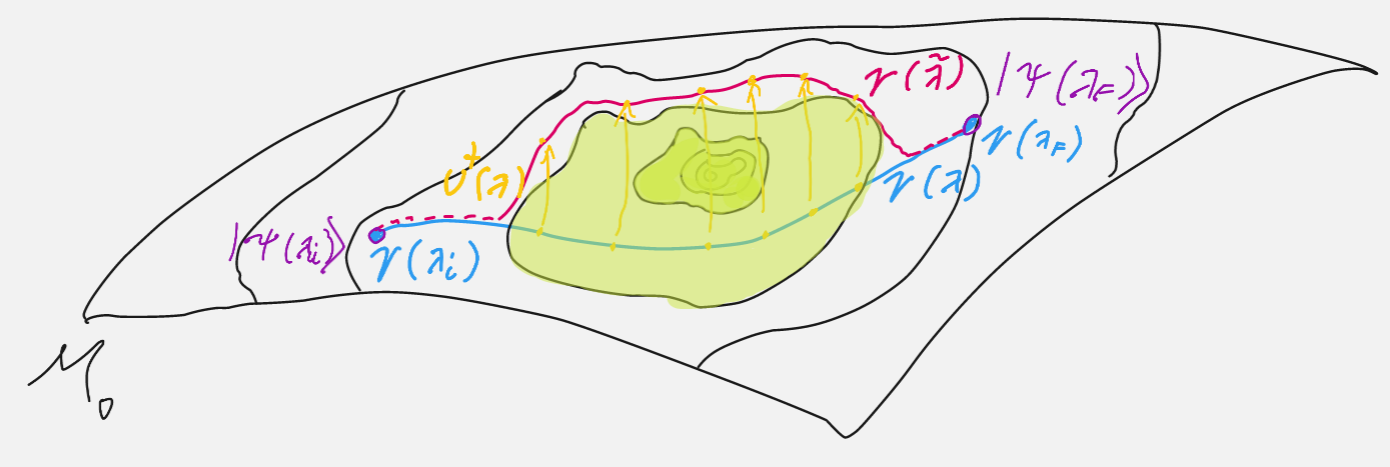
\includegraphics[width=\textwidth]{../img/counterdiabaticPotential.png}
%     \caption{Comparison between transport by Hamiltonian $\HH$ (blue path $\gamma(\lambda)$ and the one with counter-diabatic potential added (pink path $\gamma(\tilde\lambda)$), which has zero fidelity. The nonzero fidelity area for path $\gamma(\lambda)$ is marked green and initial and final states $\ket{\psi(\lambda_i)}$, resp. $\ket{\psi(\lambda_f)}$ are marked purple.}
%     \label{fig:counterdiabaticPotential}
% \end{figure}
This procedure does not directly tell us how to calculate the counter-diabatic potential, only states its existence. For many simple cases the calculation can be done analytically, but most often some approximation methods are needed.


\subsubsection{Explicit form}
If we now consider the parametrization with time $t\coloneqq t$, $\U$ can be explicitly expressed according to \textcolor{red}{ansatz} in eq. \ref{eq:phasesOnManifold} as
\begin{equation}
    \U(t)=\sum_n \exp\left(\frac{i}{\hbar}E_n(\tau)\d \tau - \int_0^t \braket{s(\tau)|\partial_\tau n(\tau)}\d\tau\right)\ket{s(t)}\bra{s(0)}.
    \label{eq:evolutionUduringTransition}
\end{equation}
Inserting to eq. \ref{eq:schrodingerForU}, we get explicit form of the Hamiltonian, which can be decomposed into the diagonal form of the original Hamiltonian and a counter-diabatic potential
\begin{equation}
    \HH(t)=\sum_n \ket{n}E_n\bra{n}+ i\hbar \sum_n\ket{\partial_\lambda n}\bra{n}-\braket{n|\partial_\lambda n}\ket{n}\bra{n}\eqqcolon \HH_0(t)+\HH_1(t),
\end{equation}
for shortened notation $\ket{n}\equiv \ket{n(t)}$, analogically for bras. Using
\begin{equation}
    \HH_0(t)\ket{n}=E_n\ket{n}\quad \Rightarrow\quad \braket{m|\partial_\lambda n}=\frac{\braket{m|\partial_\lambda\HH_0| n}}{E_n-E_m}
\end{equation}
we have explicit formula
\begin{equation}
    \HH_1(t)= i\hbar \sum_{m\neq n}\frac{\ket{m}\braket{m|\partial_\lambda\HH_0| n}\bra{n}}{E_n-E_m}
    \label{eq:explicitCounterDiabaticPotential}
\end{equation}











% \section{\textcolor{blue}{Approximations of adiabatic potentials}}
% Adiabatic potentials can be calculated from the principal of minimal action, which leads to variational method.

% If the difference between eigenstates of $\HH$ is small, or generalized force between some states is zero, the computation of the adiabatic potential is numerically unstable. The knowledge of exact adiabatic potential would allow to maintain the system in the ground state thus not exciting it, as the Eigenstate thermalization hypotheses states.

% \begin{hypot}[Eigenstate thermalization hypotheses]
%   For the difference between eigenstates of $\HH$ and extensive thermodynamic entropy $S$, it holds that
%     \begin{equation}
%     E_n-E_m\propto \exp\left(\frac{S}{2}\right).
%   \end{equation}
%   If the states are close, better approximation would be $E_n-E_m\propto \exp(S)$. For matrix elements it holds, that they vanish exponentially with the characteristic scale of the system $a$, i.e.
%   \begin{equation}
%     \bra{m}\AA_\lambda\ket{n} = i\hbar\frac{\braket{m|\partial_\lambda \HH|n}}{E_m-E_n} \propto \exp(-a).
%     \label{eq:thermalizationMatrixElements}
% \end{equation}
% \end{hypot}
% Fortunately in the limit "number of particles" $\rightarrow \infty$ the expression in eq. \ref{eq:thermalizationMatrixElements} converges.



% \subsection{Variational methods}
% In the case of simple systems, the adiabatic potentials can be found analytically, but for more complicated Hamiltonians we will be forced to use approximations, or some perturbational and variational methods.
\chapter{Quantum state driving}
\label{chap:typesOfDriving}
The concept of quantum state driving was introduced in the previous chapter. In this chapter the initial state is chosen as eigenstate $\ket{s(\llambda)}$. The driving parameter $\llambda$ is changed along path parametrized by time $t$
\begin{equation}
    \mathcal J\coloneqq\{\llambda(t)|t\in[0,T],\; \llambda\in \mathcal U\} \subset \R^N,\quad \llambda(0)=\llambda,\; \llambda(T)=\tilde\llambda,
    \label{eq:defJ_QSdriving}
\end{equation}
inducing the change in Hamiltonian $\HH(\llambda)$ and consequently in $\ket{\psi(\llambda)}$, according to the Schr\"odinger equation. This leads to solving the system of $N$ first order differential equations with initial condition $\ket{\psi(\llambda)}=\ket{s(0)}$.

Often needs to achieve as high fidelity as possible during the driving, meaning avoiding the state excitation. If $F=1$, we speak about \emph{unit fidelity driving} or \emph{adiabatic driving} and $\mathcal J$ is called the \emph{unit fidelity protocol}. Higher fidelity can be achieved by many methods; three of them are
\begin{itemize}
    \item close adiabatic driving -- changing the driving parameters $\llambda$ slowly, so the system has plenty of time to collapse into the ground state,
    \item path variation -- varying the driving trajectory $\mathcal J$, avoiding the topological defects on manifolds, which would excite the system,
    \item counter-diabatic driving -- countering the excitation by adding some element to the Hamiltonian, making the fidelity precisely $1$.\footnote{There is a nice analogy with driving a toy car \gray{(a quantum state)} in a curved terrain \gray{(a Hilbert space)}. To avoid the car jumping on the hills \gray{(the state excitation)}, you can either drive slowly \gray{(close adiabatic driving)}, or you can go around the hills \gray{(vary the path)}, or you can alter the space for a specific driving \gray{(add a counter-diabatic element)}, such that it exactly copies the jumping trajectory, therefore the car does not leave the ground.}
\end{itemize}

Before going through individual methods, let's look at the adiabaticity itself.

\begin{definition}[Adibaticity]
    The slow change of the driving parameters of the Hamiltonian $H(\llambda)$ in a sense that it does not excite the system and allows the system to return to the same energetic state after circulation around any closed path on the ground state manifold with fidelity $F=1$. 
\end{definition}
This means that adiabatic transport is an endomorphism of $\M _s$. The meaning of the word "slow" clears up the next theorem. It defines when the distance between two states can be considered zero.
\begin{thm}[Adiabatic theorem]
    \label{adiabaticTheorem}
    For slowly varying Hamiltonian $\HH$ in the time range $[0,T]$, the solution of the Schrödinger equation 
    $$\HH(\lambda)\ket{\psi_s(\lambda)} = E_s(\lambda)\ket{\psi_s(\lambda)}$$
    with initial condition in x-representation $\braket{x|\psi(t=0}=\psi(x,0)$ can be approximated as
    \begin{equation}
      ||\psi(\lambda) - \psi_{ad}(\lambda)||\approx o\left(\frac{1}{T}\right)
    \end{equation}
    for the adiabatic state evolved according to Eq. \ref{eq:phasesOnManifold}
    \begin{equation}
        \ket{\psi_{ad}}= e^{\omega_s(\lambda)}e^{\gamma_s(\lambda)}\ket{\psi(\lambda)},
    \end{equation}
    for dynamical phase
    $$\omega_s(\lambda)\equiv -\int_0^t E_s(\tau)\d \tau$$
    and geometrical phase
        $$\gamma_s(\lambda)\equiv \int_0^t i\braket{\psi_s(\tau)|\partial_t\psi_s(\tau)} \d \tau .$$
\end{thm}
\begin{myproof}
    The proof can be found in \citet{sakurai}[chap. 6].
\end{myproof}














\section{Counter-diabatic driving}

Assume differentiable and non-singular Hamiltonian $\HH(\llambda)$ with non-degenerate eigenbasis $\{\ket{s,\llambda}\}_{s=0}^{N-1}$ called the \emph{adiabatic basis}. This is generally the family of adiabatically connected eigenstates\footnote{In the case of energy level crossing, the eigenstates are not unified, because transition between them is not adiabatic.} The transition amplitude between states for adiabatic change is
\begin{equation}
    0=\bra{m(\llambda)}\HH\ket{s(\tilde\llambda)} \quad \text{for }s\neq m, \forall \llambda,\forall \tilde \llambda.
\end{equation}
Differentiation by $\partial_t$ yields
\begin{equation}
    \begin{split}
        0&=\bra{\partial_t m(\llambda)}\HH(\tilde \llambda)\ket{s(\tilde\llambda)}+ \bra{m(\llambda)}\overbrace{\partial_t\HH(\tilde \llambda)}^{\approx \partial_t\HH(\llambda)}\ket{s(\tilde\llambda)}+ \bra{m(\llambda)}\HH(\tilde \llambda)\ket{\partial_t s(\tilde \llambda)}\\
        &=E_s(\lambda)\braket{\partial_t m(\llambda)|s(\tilde \llambda)} + E_m(\lambda)\braket{m(\llambda)|\partial_t s(\tilde \llambda)}+ \bra{m(\llambda)}\partial_t \HH(\tilde\llambda)\ket{s(\tilde \llambda)}\\
        &= (E_m(\lambda)-E_s(\lambda))\underbrace{\braket{m|\partial_t s(\tilde \llambda)}}_{-\frac{i}{\hbar}\bra{m}\AA_t\ket{s(\tilde \llambda)}} + \braket{m|\partial_t\HH|s(\tilde \llambda)},
    \end{split}
\end{equation}
which can be rewritten in matrix form as
\begin{equation}
    i\hbar\partial_t\HH=[\AA_t,\HH]-i\hbar \hat{M}_t\qquad \text{for } \hat{M}_t\equiv -\sum_s\pder{E_s(\lambda)}{t}\ket{s(\lambda)}\!\!\bra{s(\lambda)}.
\end{equation}
$\hat{M}$ is diagonal in energetic basis and its elements has meaning of \emph{generalized force}. We can see that $[\HH,\hat{M}]=0$, implying
\begin{equation}
    [\HH,i\hbar\partial_t\HH-[\AA_t,\HH]]=0.
    \label{eq:komutation}
\end{equation}
This equation is essentially the system with constraint $\AA_t$. Its strength lies in the fact that it finds the counter-diabatic potential without Hamiltonian diagonalization. For more, see \citet[Chap. 2.3]{kolodrubez}.










% \subsection{The Hamiltonian gauge transformation}
In section \ref{sec:derivationOfGeometricTensor} we introduced the gauge potential and stated its correspondence to transition probability, see Eq. \ref{eq:probabilityOfTransitionIsGauge}.
\emph{Gauge transformations}, in classical mechanics called \emph{canonical}, can be defined such that they \emph{preserve Lagrangian of the system under local transformations from some Lie group}. The implication is that Hamiltonian $\HH(\llambda)$ commutes with its canonically transformed version.

To understand the meaning of gauge symmetries, let's first consider classical systems and then move to quantum mechanics.




\subsection{Classical gauge potential}
This part is inspired by \citet[Chap. 2.1]{kolodrubez}. In the Hamiltonian classical mechanics, the manifold $\M$ is assumed to be a subset of the phase space defined by Hamiltonian $H=H(q^i,p_i)$, where momentum $p_i$ and position $q^i$ are assumed to form the orthogonal basis of the phase space
\begin{equation}
    \{q^i,p_j\}=\delta^i_j,
    \label{eq:canonicalCommutationDelta}
\end{equation}
which also defines \emph{calibrational freedom} in their choice. \emph{Canonical transformations} then by definition preserve this formula. Using the \emph{Poisson bracket}, defined on observables as
\begin{equation}
    \{A,B\}\coloneqq \pder{A}{q^j}\pder{B}{p_j}-\pder{B}{q^j}\pder{A}{p_j},
\end{equation}
we examine continuous canonical transformations generated by gauge potential $\A_\lambda$
\begin{align}
        q^j(\lambda+\delta\lambda)&=q^j(\lambda)-\pder{\A_\lambda(\bm{p},\bm{q})}{p_j}\delta\lambda \;\Rightarrow\; \pder{q^j}{\lambda}=-\pder{\A_\lambda}{p_j}=\{\A_\lambda,q^j\}
        \label{eq:gaugeAsGeneratorOfMotion1}\\
        p_j(\lambda+\delta\lambda)&=p_j(\lambda)-\pder{\A_\lambda(\bm{p},\bm{q})}{q^j}\delta\lambda \;\Rightarrow\; \pder{p_j}{\lambda}=-\pder{\A_\lambda}{q^j}=\{\A_\lambda,p_j\}.
        \label{eq:gaugeAsGeneratorOfMotion2}
\end{align}
Substituting this to relations of orthogonality \ref{eq:canonicalCommutationDelta}, we get
\begin{equation}
    \{q^j(\lambda+\delta\lambda),p_j(\lambda+\delta\lambda)\}=\delta^i_j + \mathcal{O}(\delta\lambda^2).
\end{equation}
 
If $\lambda$ is time parameter and $\A_t=-H$, equations \ref{eq:gaugeAsGeneratorOfMotion1},\ref{eq:gaugeAsGeneratorOfMotion2} are identical to the Hamilton equations
\begin{equation}
\begin{split}
    \dot{q}^j&=\{q^j,H\} = \pder{H}{p_j}\\
    \dot{p}_j&=\{p_j,H\} = -\pder{H}{q^j}.
\end{split}
\end{equation}
Because the Hamiltonian is a generator of the movement in the phase space $(\bm{q},\bm{p})$, we can interpret $\A_t$ as the generators of the movement on $\M$. Another specific choice might be $\lambda=q^i$, which gives us the momentum components $\A_{q^i}=p_i$.



\subsection{Quantum gauge potential}
This part is inspired by \citet[Chap. 2.2]{kolodrubez}.
Now the aim is to find some special basis transformations $\U$ between the initial system $S$ and the transformed $\tilde{S}$. Both of them describe the system with Hamiltonian $\HH(\llambda)$ with eigenstates $\ket{s(\llambda)}$ on state manifolds $\P\M_s$. 

Any state of $\H(\llambda)$ for $\forall \llambda\in \mathcal U$ can be decomposed as
    \begin{equation}
    \ket{\psi(\llambda)}\equiv \sum_s \psi_s(\llambda)\ket{s}
\end{equation}    
for some coordinate independent basis $\{\ket{s}\}_{s=0}^{N-1}$.
Then there exist unitary transformation
\begin{equation}
    \U(\llambda): \tilde S\rightarrow S,\quad \U(\llambda)\ket{m(\llambda)}=\ket{s}.
    \label{eq:transformationU}
\end{equation}
where scalar parameter $\llambda(t)$ is assumed to be changing along the path $\mathcal J$, therefore we can write the Hamiltonian and states only as functions of $t$. The unitary transformation then satisfies
\begin{equation}
    i\hbar \partial_t \U(t)=\HH(t)\U(t)
    \label{eq:schrodingerForU}
\end{equation}
for $\HH$ the full Hamiltonian of the system and any point on $\mathcal J$, along which the partial derivative is taken.


% The wave function $\kpsi$ in $S$ can be decomposed using Schmidt decomposition\footnote{The Schmidt decomposition can be performed in finite dimension, or if the Hamiltonian is compact, which is not automatic in quantum mechanics. What's more, the Hamiltonian is usually not even bounded. Anyway, for simple systems with bounded energy we can assume so.}
% \begin{equation}
%     \ket{\psi(\llambda)} = \sum_{m,s}\psi_n(\llambda) \ket{m(\llambda)}\overbrace{\braket{m(\llambda)|s}}^{U_{ms}(\llambda)} =\sum_m \overbrace{\tilde{\psi}_m(\llambda)}^{\braket{m(\llambda)|\psi_n|s}}\ket{m(\llambda)},
% \end{equation}
% where $U_{ms}(\llambda)$ are matrix elements of unitary transformation $\U(\llambda)$. In this work, we will be interested only in the gauge transformations preserving energy of the system.





% \subsubsection{Adiabatic gauge potential}
The generators of unitary transformations are the adiabatic potentials, which can be defined on wave function $\ket{\tilde\psi(\llambda)}$ defined in system $\tilde S$, as
\begin{equation}
    i\hbar\partial_\lambda \ket{\tilde{\psi}(\llambda)} = i\hbar \partial_\lambda\left(\U^+(\llambda)\ket{\psi} \right)= \underbrace{i\hbar\left(\partial_\lambda \U^+(\llambda)\right)\U(\llambda)}_{-\tilde{\AA_\lambda}}\ket{\tilde{\psi}(\llambda)}.
\end{equation}
The adiabatic potential $\tilde{\AA_\lambda}$ can be transformed to non-tilde system as
\begin{equation}
    \begin{split}
        \AA_\lambda&=\U(\llambda)\tilde{\AA_\lambda}\U^+(\llambda) = -i\hbar\U(\llambda)\big(\partial_\lambda \U^+(\llambda)\big) =\\
        &= -i\hbar\partial_\lambda\big(\underbrace{\U^+(\llambda)\U(\llambda)}_{\mathds{1}}\big)-\big(\partial_\lambda \U(\llambda)\big)\U^+(\llambda) \big) =i\hbar \big(\partial_\lambda \U(\llambda\big)\U^+(\llambda).
    \end{split}
\end{equation}
Now we have explicit formulas for adiabatic potential in two systems
\begin{align}
    \AA_\lambda&=i\hbar \big(\partial_\lambda \U(\llambda)\big)\U^+(\llambda)
    \label{eq:adiabaticPotential}\\
    \tilde{\AA_\lambda} &= -i\hbar\left(\partial_\lambda \U^+(\llambda)\right)\U(\llambda)
    \label{eq:adiabaticPotentialTilde}
\end{align}

The adiabatic potentials can be shown to be Hermitian
\begin{equation}
     \tilde{\AA_\lambda}^+=i\hbar U(\llambda)^+\big(\partial_\lambda\U(\llambda)\big)=-i\hbar\big(\partial_\lambda\U(\llambda)^+\big)\U(\llambda) = \tilde{\AA_\lambda},
     \label{eq:counterdiabaticPotentialTwoSystems}
\end{equation}
analogically for non-tilde potential.

Using the eigenbasis of $\HH$, the matrix elements are
\begin{equation}
    \bra{s}\tilde{\AA_\lambda}\ket{m}=i\hbar\bra{s}\U(\llambda)^+\partial_\lambda\U(\llambda)\ket{m} = i\hbar\bra{s(\llambda)}\partial_\lambda\ket{m(\llambda)}.
\end{equation}
and because
\begin{equation}
    \bra{s(\llambda)}\AA_\lambda\ket{ m(\llambda)}= \bra{s}\tilde{\AA_\lambda}\ket{m},
\end{equation}
we get
\begin{equation}
    \AA_\lambda = i\hbar\partial_\lambda.
    \label{eq:adiabaticPotentialDefinition}
\end{equation}

% It's good to point out that we were applying tilde operators to non-tilde states et vice versa. This can be justified if we consider $\M$ big enough to contain all necessary states, which can be achieved during the transformation.

To see that the gauge potential performs transformation to non-exciting system, one can recall the general form of the adiabatic potential
\begin{equation}
    \bm{\mathcal A}=\big(\bm\nabla U(t)\big)U^{-1}(t) + U(t) \bm{\mathcal A} U^{-1}(t).
\end{equation}
The fact that second element is missing in Eq. \ref{eq:adiabaticPotential} implies the space has zero curvature. According to Eq. \ref{eq:geometricTensor}, the curvature is
\begin{equation}
    \chi_{jk}(\llambda) = \partial_j A_k(\llambda)-\partial_k A_j(\llambda) = 0.
\end{equation}
This means that adiabatic gauge transformations are a class of gauge transformations with $g_{jk}=\Re\chi_{jk}=0$ and according to Eq. \ref{eq:distanceOnM0}, fidelity $F=1$. Therefore the system is driven by Hamiltonian $\HH(\llambda)$ with fidelity $F<1$, there exists such adiabatic potential $\A_\lambda$, that driving of the same system using $\HH-\A_\lambda$ has unit fidelity.

The adiabatic gauge potentials can then be understood as affine connections defining the parallel transport on fiber bundle, if we define covariant derivative as
\begin{equation}
    D_j\coloneqq\partial_j+i\AA_j,
\end{equation}
which yields $D_j\ket{\psi_n}=0$ for every eigenstate, meaning the transport of eigenvalues on $\P\M_0$ is parallel. $\AA_j$ is generally defined by Eq. \ref{eq:adiabaticPotential}, which gives non-zero covariant derivative for states not belonging to $\P\M_0$. 

Calculating these potentials has many practical applications, so let's introduce one computational analytical procedure.






% \subsection{Performing counter-diabatic driving}
% This example is taken from \citet{kolodrubez}[page 15--17]. The idea of counter-diabatic driving is that any excitation of the system can be countered by adding the counter-diabatic potential to the Hamiltonian. Consider again any eigenstate $\ket{\psi(\llambda)}$ of the Hamiltonian $\HH=\HH(\llambda)$ driven along the curve $\mathcal J(\llambda(t))$ on $\P\M_0$ depending on time $t$. Because the system is not measured during the driving, it cannot be stated if or if not it was excited, but the main goal here is to achieve fidelity $F=1$, which is iff $\tilde H$ is diagonal along the driving path. For a diagonalizable Hamiltonian, there exists a transformation; see Eq. \ref{eq:transformationU}, for which the fidelity will be zero. Such transformation does not have to be unique, but we can choose any one of them. It can be seen more clearly from a direct transformation of the Schr\"odinger equation. 

% From now on assume $\llambda=\llambda(t)$. The Schrödinger equation
% \begin{equation}
%     i\hbar \der{}{t}\ket{\psi(\llambda)} = \HH(\llambda)\ket{\psi(\llambda)}
% \end{equation}
% can be transformed using 
% \begin{equation}
%     \U(\llambda)^+  \ket{\psi(\llambda)} = \ket{\tilde\psi(\tilde\llambda)},
%     \label{eq:transformationUtimeDependentH}
% \end{equation}
% for which $\tilde H \coloneqq\U^+\HH\U$ is diagonal, leading to
% \begin{align}
%     i\hbar \der{}{t}(\U(\tilde\llambda)\ket{\tilde \psi(\tilde\llambda)}) &= \HH(\llambda)\U(\tilde\llambda)\ket{\tilde \psi(\tilde\llambda)} \\
%     i\hbar \der{\llambda}{t}\partial_\llambda\U(\tilde\llambda)\ket{\tilde \psi(\tilde\llambda)} + i\hbar \U(\tilde\llambda)\der{}{t}\ket{\tilde \psi(\tilde\llambda)} &= \HH(\llambda)\U(\tilde\llambda)\ket{\tilde \psi(\tilde\llambda)}.
% \end{align}

% This can be rewritten using adiabatic potential from Eq. \ref{eq:adiabaticPotentialDefinition}, using \emph{dot} notation for time derivatives and omitting the points in which the objects are evaluated, as
% \begin{equation}
%     i\hbar \der{}{t}\ket{\tilde\psi} = \left[\U^+\HH\U-\dot{\lambda}\tilde{\AA_\lambda}\right]\ket{\tilde\psi} = \left[\tilde H-\dot{\lambda}\tilde{\AA_\lambda}\right]\ket{\tilde{\psi}} \eqqcolon \tilde{H}_m \ket{\tilde{\psi}},
% \end{equation}
% where the term $-\dot{\lambda}\tilde{\AA_\lambda}$ is called \emph{Galilean} and $ \tilde{H}_m$ is the Hamiltonian in transformed system. Because $\tilde{H}$ is diagonal, it drives $\ket{\tilde{\psi}}$ with fidelity $f=1$. This means that for any driving defined by $\HH(\lambda(t))$, which defines the unitary transformation $\U$, there exists such \emph{counter-diabatic potential} $\AA_\lambda$, that $\HH_m + \dot{\lambda}\AA_\lambda$ has $f=1$.


% % Intuition for transformations using original Hamiltonian vs. transformed one can be seen on Fig. \ref{fig:counterdiabaticPotential}. It is good to point out that the eigenstates on this figure belong to the space $\P\M$. However, the paths themselves need to be considered in the whole $\M$, which can be seen as the phase change described by equation \ref{eq:evolutionUduringTransition}.

% % \begin{figure}[h]
% %     \centering
% %     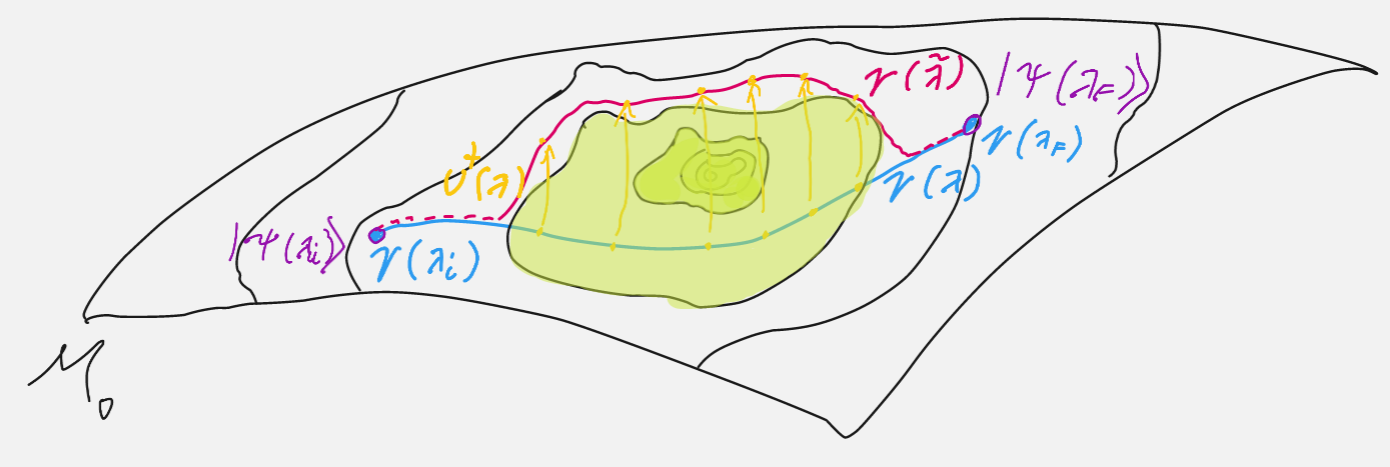
\includegraphics[width=\textwidth]{../img/counterdiabaticPotential.png}
% %     \caption{Comparison between transport by Hamiltonian $\HH$ (blue path $\mathcal J(\lambda)$ and the one with counter-diabatic potential added (pink path $\mathcal J(\tilde\lambda)$), which has zero fidelity. The nonzero fidelity area for path $\mathcal J(\lambda)$ is marked green and initial and final states $\ket{\psi(\lambda_i)}$, resp. $\ket{\psi(\lambda_f)}$ are marked purple.}
% %     \label{fig:counterdiabaticPotential}
% % \end{figure}
% This procedure does not directly tell us how to calculate the counter-diabatic potential, only states its existence. For many simple cases the calculation can be done analytically, but often some approximation methods are needed.


% % \begin{figure}[h]
% %     \centering
% %     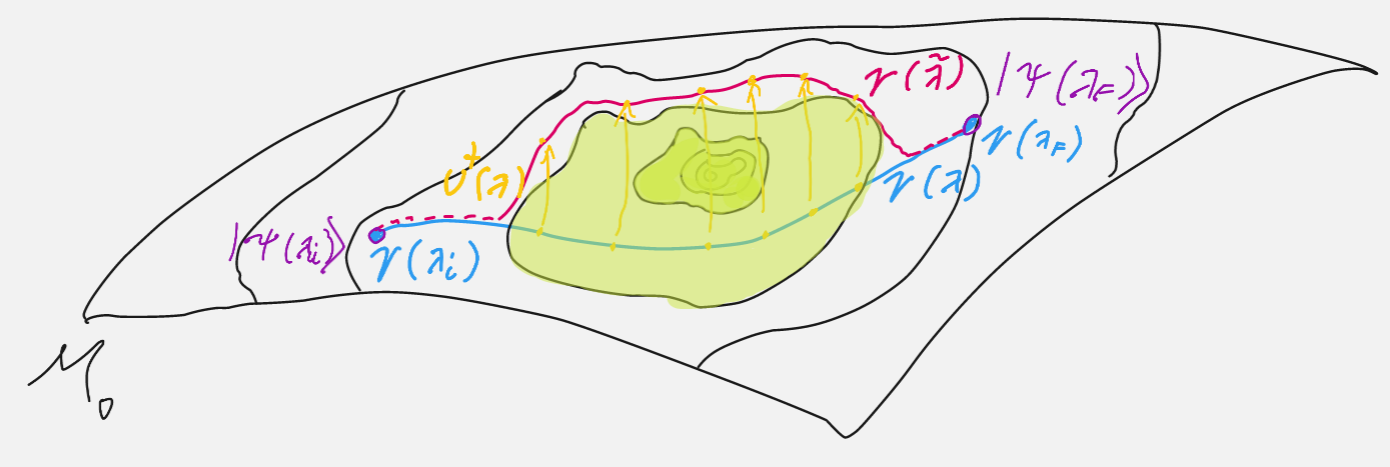
\includegraphics[width=\textwidth]{../img/counterdiabaticPotential.png}
% % \end{figure}




% \subsubsection{Explicit form}
% If we now consider the parametrization with time $t$, $\U$ can be explicitly expressed according to ansatz in Eq. \ref{eq:phasesOnManifold} as
% \begin{equation}
%     \U(t)=\sum_n \exp\left(\frac{i}{\hbar}E_n(\tau)\d \tau - \int_0^t \braket{s(\tau)|\partial_\tau n(\tau)}\d\tau\right)\ket{s(t)}\bra{s(0)}.
%     \label{eq:evolutionUduringTransition}
% \end{equation}
% Inserting to Eq. \ref{eq:schrodingerForU}, we get explicit form of the Hamiltonian, which can be decomposed into the diagonal form of the original Hamiltonian and a counter-diabatic potential
% \begin{equation}
%     \HH(t)=\sum_n \ket{n}E_n\bra{n}+ i\hbar \sum_n\ket{\partial_\lambda n}\bra{n}-\braket{n|\partial_\lambda n}\ket{n}\bra{n}\eqqcolon \HH_0(t)+\HH_1(t),
% \end{equation}
% for shortened notation $\ket{n}\equiv \ket{n(t)}$, analogically for bras. From Eq. \ref{eq:mgradn_proof} we have
% \begin{equation}
%     \HH_0(t)\ket{n}=E_n\ket{n}\quad \Rightarrow\quad \braket{m|\partial_\lambda n}=\frac{\braket{m|\partial_\lambda\HH_0| n}}{E_n-E_m}
% \end{equation}
% and the explicit formula for counter-diabatic element is
% \begin{equation}
%     \HH_1(t)= i\hbar \sum_{m\neq n}\frac{\ket{m}\braket{m|\partial_\lambda\HH_0| n}\bra{n}}{E_n-E_m}
%     \label{eq:explicitCounterDiabaticPotential}
% \end{equation}
























\section{Driving on the ground state manifold}
\label{chap:groundStateManifoldDriving}
As was mentioned in the introduction of chapter \ref{chap:typesOfDriving}, one method of achieving low driving fidelity is \emph{path variation}. It means \emph{finding the best possible driving path}. One might say that the ground state manifold geodesics are a good candidate for this path because they minimize the distance. The problem is that general fidelity driving does not happen on any state manifold, and this premise cannot be used. The natural question here is: "For which drivings do geodesics minimize the fidelity?". The whole role of geodesics is not yet known, but there are a few known cases in which they have particular meaning and which are demonstrated here.

\subsection{Minimizing the distance on state manifolds}
Let's have path $\mathcal J$ defined in Eq. \ref{eq:defJ_QSdriving} and a geodesic $\mathcal G(\llambda(t))$ with fixed boundary conditions
 $$\mathcal{G}(0)=\mathcal J(0),\qquad \mathcal{G}(T)=\mathcal J(T).$$

The driving on projective ground state manifold $\P\M_0$ then consists of infinitesimal quenches over the distance $\d s$. By integration over this path we get the distance
\begin{equation}
    s_{\mathcal J}=\int\limits_{\mathcal J}\d s=\int\limits_{0}^{T}\sqrt{g_{jk}\dot\llambda^j\dot\llambda^k}\d t
    \label{eq:distancesgamma}
\end{equation}
Let's state and prove the theorem demonstrating the importance of geodesics.
\begin{thm}
    The distance described by formula \ref{eq:distancesgamma} is minimized if $\mathcal J$ is a geodesic.
\end{thm}

\begin{proof}
    Functional of distance is
    \begin{equation}
        s=\int\limits_0^{T} \sqrt{g_{jk}\d\llambda^j\d\llambda^k}=\int\limits_0^{T} \sqrt{g_{jk}\der{\llambda^j}{t}\der{\llambda^k}{t}}\d t \eqqcolon \int\limits_0^{T} \mathcal{L}(t,\llambda^j,\dot\llambda^j)\d t
    \end{equation}
    for 
    \begin{equation}
        \mathcal{L}=\sqrt{g_{jk}\dot\llambda^j\dot\llambda^k}.
    \end{equation}
    Using Euler-Lagrange equations 
    \begin{equation}
        \der{\mathcal{L}}{\llambda^j}-\der{}{t}\der{\mathcal{L}}{\dot\llambda^j}=0,
    \end{equation}
    we get for $g_{jk}=g_{jk}(\llambda)$ second order differential equation
    \begin{equation}
        \ddot\llambda^j+\Gamma^j_{\;\;ab}\dot\llambda^a\dot\llambda^b=0\qquad \Gamma^j_{\;\;ab}=\frac{1}{2}g^{jk}\left(g_{ka,b}+g_{kb,a}-g_{ba,k}\right),
        \label{eq:geodesicEquaiton}
    \end{equation}
    which is the Geodesic equation.
\end{proof}




% \textcolor{blue}{Polkovnikov for some special case: They play a role of "maximum fidelity at any time" transport, meaning at any given time $t$ the fidelity on corresponding point on geodesics will be less than of $\mathcal J$
% $$F(\mathcal{G}(t))<F(\mathcal J(t)).$$ }







\subsection{Minimizing the energy variance}
The driving can be restricted to the ground state manifold only in approximation, such that the excited parts of the wave function can be neglected in every step. This fact is used for so-called \emph{close adiabatic drivings}. The first theorem about geodesics is from \citet{Bukov2019}.

\begin{thm}
    \label{thm:polkovnikov}
    For any fast-forward Hamiltonian\footnote{The system is driven to the target state in some fixed final time $T$.} $\HH(\lambda(t))$ driven along one dimensional path $\lambda: \R\mapsto \R$ using time $t$ as parametrization, there exist driving speed, for which the fidelity is close to one, $F(t)\approx 1, \;\forall t\in[0,T]$, and the energy fluctuations $\delta E^2$, averaged along the path, are larger than the geodesic length $l_\lambda$
    \begin{equation}
        \int\limits_0^{T}\sqrt{\delta E^2(t)}\d t \eqqcolon l_t\geq l_\lambda \coloneqq \int\limits_{\lambda_i}^{\lambda_f} \sqrt{g_{\lambda\lambda}\d \lambda\d \lambda} =\int_0^{T} \sqrt{g_{\lambda\lambda}}|\dot \lambda|\d t.
    \end{equation}
    The length $l_\llambda$ is defined in parametric space. For energy variance it holds
    \begin{equation}
        \delta E^2\coloneqq \braket{o(t)|\HH(t)^2|o(t)}-\braket{o(t)|\HH(t)|o(t)}^2=\braket{\partial_t  o(t)|\partial_t o(t)})_c=G_{tt},
    \end{equation}    
    where in second equality the Schr\"odinger equation is used. 
    
    The Metric tensor in parametric space is defined as
    \begin{equation}
        g_{\lambda\lambda}\coloneqq \braket{\partial_\lambda o(t)|\partial_\lambda o(t)})_c,
    \end{equation}
    see chapter \ref{chap:metricTensor}
\end{thm}


\begin{proof}
    The essential realization is
    \begin{equation}
        \delta E^2\equiv \braket{o(t)|\HH(t)^2|o(t)}_c=\dot\lambda^2 G_{\lambda\lambda}+\O(\dot\lambda^4),
    \end{equation}
    where $\O(\dot\lambda^4)$ needs to be positive for any real-valued Hamiltonian. The positivity comes from the fact, that the system has instantaneous time-reversal symmetry. For details see \citet{Bukov2019}.
\end{proof}

The conjecture can be extended to an arbitrary dimensional path. The main problem of this conjecture is the statement \emph{close unit fidelity protocol}. It is not clear how good the approximation needs to be. This makes the statement much weaker because it only states that \emph{for any driving, there exists nonzero driving speed for which the energy variance is minimized on geodesics.}









\subsection{Transport using quenches}
\label{sec:quenches}
Unifying the ground states $\ket{o(\llambda)}$ over all points $\llambda\in\mathcal U$ in parametric space, we get the ground state manifold. Here the fidelity $F$ and distance $s$ are
\begin{equation}
    \d s^2 = 1-F(\llambda+\delta\llambda,\llambda) = 1-\left|\braket{o(\bm\llambda+\delta\bm\llambda)|o(\bm\llambda)}\right|^2.
    \label{eq:distanceOnM0_1}
\end{equation}

The final fidelity of transport on $\M$ is then
\begin{equation}
    F=\iint\limits_{\mathcal J} g_{jk}\d\llambda^j\d\llambda^k = \int_{t_i}^{t_f}\underbrace{\int_{t_i}^\tau g_{jk}\der{\llambda^j}{t}\der{\llambda^k}{t} \d t}_{\mathcal{L}(\llambda,\dot\llambda,\tau)}\d \tau .
\end{equation}
From Euler-Lagrange equations, the fidelity is minimized if $\mathcal J$ is geodesic. It is worth mentioning the same problem as was with Theorem \ref{thm:polkovnikov}. It is only stated here that \emph{there exist such slow driving, that the fidelity is minimized on geodesics}. Not how slow this driving needs to be. 
% Using Euler-Lagrange equations for time-independent $g_{jk}=g_{jk}(\llambda)$, leads to
% \begin{equation}
%     \int_{t_i}^{\tau}\left[g_{jk,l}\dot\llambda^j\dot\llambda^k - \der{}{t}\left[g_{jl}\left(\delta^j_k\dot\llambda^k+\dot\llambda^j\delta^k_k\right)\right]\right]\d t=0,
% \end{equation}
% which needs to be zero for integration over any subset $(t_i,\tau)$. This can be achieved for any path only if the integrand itself is zero, which happens if the geodesic equation is satisfied.

% The fidelity $F$ measures transition probability between two eigenstates, $\ket{\psi_1}$, $\ket{\psi_2}$, of different Hamiltonians at two different points $\llambda_1$, $\llambda_2$. These two states belong to the same Fiber space $\PH(\llambda)$ from which the coefficients $$(\text{index of energy state $s$}; \llambda)\in (\Z,\mathcal U)$$ are taken. Because $\PH(\llambda)$ are canonically isomorphic for $\forall \llambda\in \mathcal U$, there is no problem in parallel transport from one space to another, which is needed for evaluating the braket $\braket{\psi(\llambda_1)|\psi(\llambda_2)}$. This is important because the integration in braket can be performed only if both elements belong to the same space.

% The distance minimization runs into some interpretation problems. On the one hand, minimization of the distance is equivalent to maximization of the sum of infinitesimal fidelities along the path (we say we \emph{maximize the fidelity along the path}). On the other hand, we are using only ground states in every step of the transport, therefore defining the fidelity to be one. There are two ways out of this confusion. \emph{Perturbed adiabatic driving} and \emph{transport using quenches}.


Imagine at every point of transport that the fidelity is small enough, so for some small parameters $\Delta_i\in \C$ the transport over distance $\d s$ in eigenbasis at time $t=0$ is
$$\ket{o(\llambda_i)}\equiv \begin{pmatrix}
    Z_0(\llambda_i)\\
    0\\
    \vdots \\
    0
\end{pmatrix} \overset{\text{transport }\d s}{\longrightarrow} \ket{o(\llambda_i+\delta \llambda)}\equiv\begin{pmatrix}
    Z_0(\llambda_i+\delta \llambda)\\
    0\\
    \vdots \\
    0
\end{pmatrix} +\underbrace{\begin{pmatrix}
    0\\
    \Delta_1(\llambda_i+\delta \llambda)\\
    \vdots \\
    \Delta_n(\llambda_i+\delta \llambda)
\end{pmatrix}}_{\mathbf{\Delta}(\llambda_i+\delta \llambda)}, $$
where the last term is neglected, because
$$\braket{\Delta(\llambda)|o(\llambda+\delta\llambda)}\approx 0.$$

This might have interesting implications for slow transports or small distance transports. For slow transport, this condition is hardly fulfilled because one needs to neglect the sum of many of these terms. One possible way out of this is to reset the state into the ground-state when the fidelity would get too far from 1. It can be achieved by projecting the state $\ket{\psi(t)}$ to the ground state $\ket{o(t)}$ periodically, such that every time the fidelity is almost one. These small jumps are sometimes called \emph{quenches}, and they can be achieved by introducing thermalization to the system.






If we imagine $\delta\llambda$ to be finite (not infinitely small, as the notation suggests), the \emph{transport} means \emph{doing a sequence of quenches and measuring the system after every quench}. This consequently leads to the unit fidelity transport.
% This leads to the \emph{quantum Zeno effect}. In this case it can be shown directly by splitting the distance $s$ on parametric space $\mathcal U$ to $n$ equal pieces. The fidelity for $n$ splits is then
% \begin{equation}
%     F(n)=(1-\Delta s)^n=\left(1-\left(\frac{s}{n}\right)^2\right)^n \;\;\overset{n\rightarrow\infty}{\longrightarrow}\;\; 1,
% \end{equation}
% meaning the consequent measurements on the system leads to collapse to the instantaneous eigenstate and the adiabatic condition for transport holds ($F=1$). 

% Such measurements can be achieved by fast thermalization of the system. If the finite speed thermalization with $N=T/\tau$ for the mean time between two measurements $\tau$, we get
% \begin{equation}
%     \begin{split}
%         \log f(N) &= N \log \left(1-\left(\frac{s}{N}\right)^2\right) = -\frac{s^2}{N}+o\left(\frac{s^4}{n^3}\right)\\
%         f(N) &= \exp\left(-s^2\frac{\tau}{T}-\frac{s^4}{2 N^3}\dots\right) = \exp\left(-s^2\frac{\tau}{T}\right)\left(1+o\left(\frac{s^4}{N^3}\right)\right)
%     \end{split}
% \end{equation}












\section{Adiabatic perturbation theory}
Until now, our interest was mainly in \emph{unit fidelity protocols}. But how to calculate the case when the fidelity is "almost one"? This is the aim of \emph{adiabatic perturbation theory}.


Following the article from \citet{Rigolin2008}, the wave function can be approximated by series. Because every element is then decomposed into another series, we bear in mind the \emph{locality of variables}, which clarifies the reason for performing this procedure. Let's call variable $V(t)$ \emph{\bluee{local}} if it does not depend on driving path. These variables are in shades of \bluee{blue} and \redd{non-local} variables, written in shades of \redd{red}, are usually expressed as an integral over driving path $\mathcal J$.

We are interested in the driving along path $\mathcal J$ defined by Eq. \ref{eq:defJ_QSdriving},
where $t$ is time and $T$ final time of the driving. Let the initial condition be
\begin{equation}
    \ket{\psi(0)}\eqqcolon\ket{\psi_0}\in \P\M_0.
\end{equation}
Solving the Schr\"odinger equation might seem like a straightforward solution. However, if the fidelity is close to 1, the approximate methods are, in comparison with numerical methods, relatively stable. Second reason is, that they might result in an analytical solution to the problem.

The power series is derived using a small parameter $v\coloneqq 1/T$
\begin{equation}
    \red{\ket{\Psi(t)}}=\sum_{p=0}^\infty v^p \red{\ket{\Psi^{(p)}(t)}},
    \label{eq:mainSeries}
\end{equation}
for 
\begin{equation}
    \red{\ket{\Psi^{(p)}(t)}}=\sum_{s=0}^{N-1} e^{-\frac{i}{v} \reddd{\omega_s(t)}}e^{i\reddd{\gamma_s(t)}}\redd{b_s^{(p)}(t)}\bluee{\ket{s(t)}}.
\end{equation}
Here we have
\begin{align}
    \text{dynamical phase }\reddd{\omega_s(t)} &\coloneqq \frac{1}{\hbar}\int_0^t \bluee{E_s(\tau)}\d \tau,\\
    \text{Berry phase }\reddd{\gamma_s(t)} &\coloneqq i\int_0^t \bluee{\braket{s(\tau)|\frac{\d}{\d \tau}s(\tau)}}\d \tau \equiv i\int_0^t \bluee{M_{ss}(\tau)}\d \tau
    \label{eq:gammadef}
\end{align}
and $\bluee{\ket{s(t)}}$ are solutions to
\begin{equation}
    \bluee{\HH(t)\ket{s(t)}}=\bluee{E_s(t) \ket{s(t)}}.
\end{equation}
Variables $\reddd{\omega_s(t)}$ and $\reddd{\gamma_s(t)}$ are defined using integration over the whole protocol, therefore they are \emph{\red{non-local variables}}.
The problem now lies in determining $\redd{b_s^{(p)}(t)}$, which is also \red{non-local}. Because it depends on its relative \reddd{geometric} and \reddd{dynamical phase} to other \bluee{energy levels}, let's write it as a series
\begin{equation}
    \redd{b_s^{(p)}(t)}=\sum_{m=0}^{N-1} e^{\frac{i}{v}\reddd{\omega_{sm}(t)}}e^{-i\reddd{\gamma_{sm}(t)}}\blue{b_{sm}^{(p)}(t)},
    \label{eq:bnAPT}
\end{equation}
where $\reddd{\omega_{sm}} \coloneqq \reddd{\omega_m}-\reddd{\omega_s}$, $\reddd{\gamma_{sm}} \coloneqq \reddd{\gamma_m}-\reddd{\gamma_s}$.  The reason for \blue{locality} of $\blue{b_{sm}^{(p)}(t)}$ will be clear soon.

Inserting all to original series \ref{eq:mainSeries}, we get
\begin{equation}
    \red{\ket{\Psi(t)}}=\sum_{s,m=0}^{N-1}\sum_{p=0}^\infty v^p e^{-\frac{i}{v}\reddd{\omega_m(t)}}e^{i\reddd{\gamma_m(t)}}\redd{b_{sm}^{(p)}(t)}\bluee{\ket{s(t)}}.
    \label{eq:solve0}
\end{equation}

Because the initial state is an eigenstate of the Hamiltonian at time $t=0$, we get initial condition $\blue{b_{sm}^{(0)}(t)=0}$. In addition, one can rewrite equation \ref{eq:solve0} to the iteratively solvable form
\begin{equation}
    \frac{i}{\hbar}\bluee{\Delta_{sm}(t)}\blue{b_{sm}^{(p+1)}(t)}+\blue{\dot b_{sm}^{(p)}(t)}+\bluee{W_{sm}(t)} \blue{b_{sm}^{(p)}(t)}+\sum_{k=0,k\neq s}\bluee{M_{sk}(t)}\bluee{b_{km}^{(p)}(t)}=0,
    \label{eq:bSolution}
\end{equation}
for $\bluee{\Delta_sm(t)}\coloneqq \bluee{E_m-E_s}$, $\bluee{W_{sm}(t)}\coloneqq \bluee{M_{ss}(t)}-\bluee{M_{mm}(t)}$, where $\bluee{M_{ms}}$ is defined in Eq. \ref{eq:gammadef}. We can see that $\blue{b_{ms}^{(p)}}$, as a solution to Eq. \ref{eq:bSolution}, only depends on difference between energy levels, eigenstates during the path and their directional derivatives. Not on the path itself. All of these are easily obtained, once the driving path is prescribed.















% \section{\textcolor{blue}{Approximations of adiabatic potentials}}
% Adiabatic potentials can be calculated from the principal of minimal action, which leads to variational method.

% If the difference between eigenstates of $\HH$ is small, or the generalized force between some states is zero, the computation of the adiabatic potential is numerically unstable. The knowledge of exact adiabatic potential would allow to maintain the system in the ground state thus not exciting it, as the Eigenstate thermalization hypotheses state.

% \begin{hypot}[Eigenstate thermalization hypotheses]
%   For the difference between eigenstates of $\HH$ and extensive thermodynamic entropy $S$, it holds that
%     \begin{equation}
%     E_s-E_m\propto \exp\left(\frac{S}{2}\right).
%   \end{equation}
%   If the states are close, better approximation would be $E_s-E_m\propto \exp(S)$. For matrix elements it holds, that they vanish exponentially with the characteristic scale of the system $a$, i.e.
%   \begin{equation}
%     \bra{m}\AA_\lambda\ket{n} = i\hbar\frac{\braket{m|\partial_\lambda \HH|n}}{E_m-E_s} \propto \exp(-a).
%     \label{eq:thermalizationMatrixElements}
% \end{equation}
% \end{hypot}
% Fortunately in the limit "number of particles" $\rightarrow \infty$ the expression in Eq. \ref{eq:thermalizationMatrixElements} converges.



% \subsection{Variational methods}
% In the case of simple systems, the adiabatic potentials can be found analytically, but for more complicated Hamiltonians we will be forced to use approximations or some perturbational and variational methods.
% \chapter{\textcolor{blue}{Spin 1/2}}
The Hamiltonian for a single spin in a magnetic field $\mathbf B$ is
\begin{equation}
    H=-\mu\mathbf B \cdot \mathbf S
\end{equation} 
for spin $1/2$ we have using sigma matrices
\begin{equation}
    S=\frac{\hbar}{2}\left(\sigma_x,\sigma_y,\sigma_z\right) \equiv \frac{\hbar}{2}\left(\left(
\begin{array}{cc}
 0 & 1 \\
 1 & 0 \\
\end{array}
\right),\left(
\begin{array}{cc}
 0 & -i \\
 i & 0 \\
\end{array}
\right),\left(
\begin{array}{cc}
 1 & 0 \\
 0 & -1 \\
\end{array}
\right)\right)
\end{equation}

The coordinate system can be oriented such that $\mathbf B=(0,0,B_z)$ and eigenfunctions of the spin are thus in spherical coordinates $\theta,\phi$ and x-representation
\begin{align}
    u_1=\begin{pmatrix}
        \cos\frac{\theta}{2}e^{-i\phi}\\
        \sin\frac{\theta}{2}
    \end{pmatrix};\qquad
    u_2=\begin{pmatrix}
        -\sin\frac{\theta}{2}e^{-i\phi}\\
        \cos\frac{\theta}{2}
    \end{pmatrix}
\end{align}
For both of these states the Berry connection can be defined using \ref{eq:berryConnection}
\begin{equation}
   A^{(u_1)} = \begin{pmatrix}
    \braket{u_1| \der{u_1}{\theta}}\\
    \braket{u_1| \der{u_1}{\phi}}
   \end{pmatrix};\qquad 
   A^{(u_2)} = \begin{pmatrix}
    \braket{u_2| \der{u_2}{\theta}}\\
    \braket{u_2| \der{u_2}{\phi}}
   \end{pmatrix}
\end{equation}
and geometric tensor using \ref{eq:geometricTensor} we have
\begin{equation}
    \chi^{(u_k)}_{ij} = 
        \braket{\partial_i u_k|\partial_j u_k}-\braket{\partial_i u_k| u_k}\braket{u_k|\partial_j u_k} 
\end{equation}
implying
\begin{equation}
    \chi^{(u_1)} = \begin{pmatrix}
        \frac{1}{4}& \frac{i}{4}\sin\theta\\
        -\frac{i}{4}\sin\theta&\frac{\sin^2\theta}{4}
    \end{pmatrix};\quad 
    \chi^{(u_2)} = \begin{pmatrix}
        \frac{1}{4}& -\frac{i}{4}\sin\theta\\
        \frac{i}{4}\sin\theta&\frac{\sin^2\theta}{4}
    \end{pmatrix}.
\end{equation}
It's real part is according to \ref{eq:metrictensorREdefinition} the metric tensor
\begin{equation}
    g^{(u_1)} = g^{(u_2)} =\begin{pmatrix}
        \frac{1}{4}& 0\\
        0&\frac{\sin^2\theta}{4}
    \end{pmatrix}
\end{equation}
\textcolor{red}{For two state system, the metric tensor is always the same for both states. (just guessing now :).} Berry curvature can be easily calculated as minus imaginary part of the geometric tensor. 

\textcolor{blue}{
From the metric the Ricci curvature and Gaussian curvature are
\begin{align}
    R&=\begin{pmatrix}
        1&0\\
        0&\frac{1}{4}\sin^2\theta
    \end{pmatrix}\\
    K&=\frac{1}{8}(1+\sin^4\theta)
\end{align}
}

If the magnetic field is positive, $u_1$ is the ground state. The metric on $\M_0$ is then $g^{(u_1)}$ calculated above. During some arbitrary change of magnetic field whilst not measuring the state of the system, it can be transported from $\ket{\psi_i}\coloneqq \ket{u_1}$ to some new ground state by changing the magnetic field direction, as shown on fig. \ref{fig:blochArbitraryTransport}
\begin{figure}[h]
    \centering
    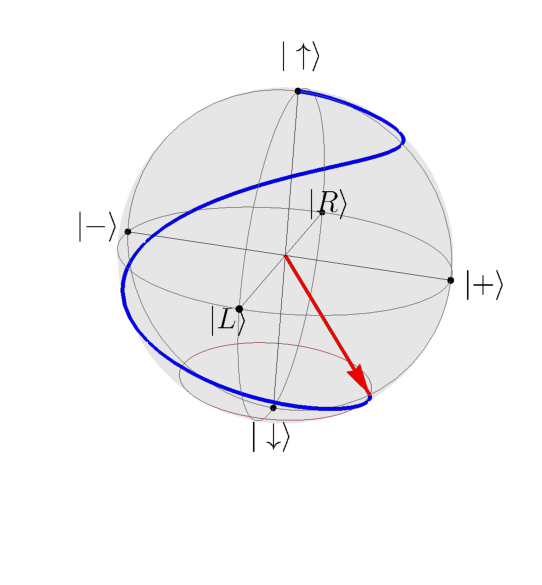
\includegraphics{../img/blochArbitraryTransport.pdf}
    \caption{Bloch sphere for the eigenstate $u_1$ with the initial direction of magnetic field $\mathbf B=(0,0,B_z)$ transported along $\gamma=\{(\phi,\sqrt{\phi})|\phi\in[0,2\pi]\}$ (blue). The final orientation of the magnetic field is marked red and the states on the Bloch sphere correspond to initial eigenstate.}
    \label{fig:blochArbitraryTransport}
\end{figure}

It's pedagogical to point out the correspondence to figure \ref{fig:manifoldCutIntuition}, where $\M_0=\cup_\llambda \{\ket{u_1}\}$,  $\M_1=\cup_\llambda \{\ket{u_2}\}$, $\ket{o(\llambda)}=u_1(\mathbf B=B(0,0))$ and $\ket{o(\tilde\llambda)}=u_1(\mathbf B=B(2\pi,\sqrt{2\pi}))$, written in spherical coordinates.


If the transport is made infinitesimally slow with respect to time $t$, after every step $\d \theta$ the eigensystem has to be calculated, and we find out that the system collapses into instantaneous $u_1(t)$ state of $\H(t)$, so the fidelity at any $\theta$ is $f_0(\theta)=1$ and $\d s^2(\theta)=1-f_0^2=0$. Opposite to the adiabatic transport would be the quantum quench, meaning the orientation of $\mathbf B$ is changed instantly resulting in a final state 
\begin{equation}
   \ket{f} = \alpha \ket{u_1} + \beta \ket{u_2}, \qquad\text{for } \frac{\alpha}{\beta}=e^{-i\phi}\tan\frac{\theta}{2},\quad \alpha^2+\beta^2=1.
\end{equation}
This yields probability of staying in the state $u_1$ after quench is $f_q=\braket{u_1|f}=\alpha$ and $s=1-\alpha$.

\section{Special case}
Assume again transport of $\ket{u_1}$ by rotating the magnetic field along the path $\gamma=\{(0,\theta)|\theta\in[0,\pi/2]\}$, as drawn on figure \ref{fig:blochPiHalfTransport}. The fidelity for infinitesimal speed is at every point on the path $f_0=1$ and for quantum quench $f_q=1/2$.

\textcolor{blue}{Now let's calculate the fidelity for some finite time transport. }
\begin{figure}[h]
    \centering
    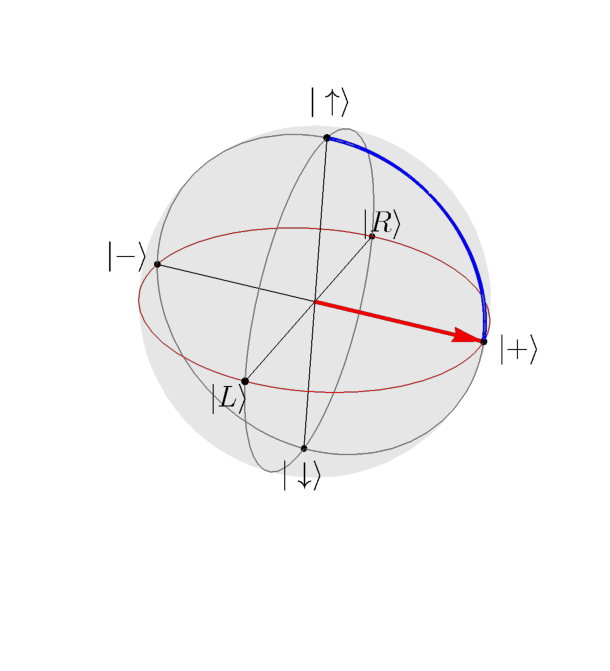
\includegraphics{../img/blochPiHalfTransport.pdf}
    \caption{Bloch sphere for the eigenstate $u_1$ with the initial direction of magnetic field $\mathbf B=(0,0,B_z)$ transported along $\gamma=\{(0,\theta)|\theta\in[0,\pi/2]\}$ (blue). The final orientation of the magnetic field is marked red and the states on the Bloch sphere correspond to initial eigenstate.}
    \label{fig:blochPiHalfTransport}
\end{figure}



\chapter{Two level system}
\label{chap:twoLevelSystem}
A simple two-level system is investigated before moving to a more complicated Hamiltonian model. To understand the general behavior of fidelity on a Hamiltonian spectrum, two analytically solvable drivings — \emph{geodesic} and \emph{linear} — are investigated.

\section{Hamiltonian}
Let's have a Hamiltonian
\begin{equation}
    \HH(t)=\begin{pmatrix}
        \Omega(t)&\Delta(t)\\
        \Delta(t)&-\Omega(t)
    \end{pmatrix}
\end{equation}
for $\Omega: \R^+\rightarrow \R$, $\Delta: \R^+\rightarrow \R$ and time $t$. Its spectrum is
\begin{equation}
    E_1(t)=-E_0(t)= \sqrt{\Omega^2(t)+\Delta^2(t)}
    \label{eq:energy}
\end{equation}
and using the eigenbasis
\begin{equation}
    \mathcal{B}\coloneqq \left\{
        \ket{0}\equiv\begin{pmatrix}
                1\\0
            \end{pmatrix},
        \ket{1}\equiv\begin{pmatrix}
            0\\1
        \end{pmatrix} \right\},
    \label{eq:eigenbasisDef}
\end{equation}
the eigenvectors  can be written as 
\begin{equation}
\ket{0(t)}=N_+ \begin{pmatrix}
    1\\ \frac{E_0(t)+\Omega(t)}{\Delta(t)}
\end{pmatrix},\quad \ket{1(t)}=N_-\begin{pmatrix}
    1\\ \frac{E_1(t)+\Omega(t)}{\Delta(t)}
   \end{pmatrix}
   \label{eq:eigenvectors}
\end{equation}
for normalization constants $N_\pm\coloneqq\left(\left(\frac{\pm E_0(t)+\Omega(t)}{\Delta(t)}\right)^2+1\right)^{-1/2}$. The instantaneous eigenbases changes in time, but is described using constant basis $\mathcal B$, which forms an eigenbasis at time $t=0$.

The goal is to find \emph{fidelity} between initial state anad state evolved along $\mathcal J$, $F_{\mathcal J}(t)\coloneqq |\braket{0(t)|\psi(t)}|^2$ for different driving protocols \begin{equation}
    \mathcal J\coloneqq\{\llambda(t)|t\in[0,T],\; \llambda\in \mathcal U\} \subset \R^N.
\end{equation}
For this we need to solve time Schr\"odinger equation
\begin{equation}
    \HH(t)\ket{\psi(t)}=i\frac{\d}{\d t}\ket{\psi(t)}
\end{equation}
with time varying Hamiltonian $\HH(\llambda(t))\eqqcolon \HH(t)$ and $\llambda$ on path $\mathcal J$. For 2-dimentional system with 
\begin{equation}
    \ket{\psi(t)}\eqqcolon \begin{pmatrix}
         a(t) \\
         b(t)    
    \end{pmatrix},
\end{equation}
we get the system of \emph{two coupled differentials equations of the first order with non-constant coefficients}
\begin{align}
    \Omega(t)a(t)+\Delta(t)b(t)&=i\dot a(t)\label{eq:a1}\\
    \Delta(t)a(t)-\Omega(t)b(t)&=i\dot b(t)
    \label{eq:a2}
\end{align}
with normalization
\begin{equation}
    a^2(t)+b^2(t)=1, \quad \forall t\in [0,T].
    \label{eq:normalizationCondition}
\end{equation}
and initial value 
\begin{equation}
    \begin{pmatrix}
        a(0)\\b(0)
    \end{pmatrix} = \ket{0(0)}.
\end{equation}















\section{Harmonic oscillator correspondence}
Coupled Equations \ref{eq:a1}, \ref{eq:a2} have no general analytical solution, with an exception to a few easy protocols $\mathcal J$. Before moving to some of these special cases, it is important to understand the general behavior of such coupled system of equations.

N-dimensional Schr\"odinger equation can be rewritten to \emph{one differential equation of N$^{th}$ order with non-constant coefficients}. In our two-dimensional case, this equation corresponds to \emph{damped harmonic oscillator without external force}
\begin{align}
    0&= \ddot a(t)+ \gamma(t) \dot a(t)+\omega^2(t)a(t) \label{eq:harmonicOscillator}\\
    \gamma(t)&\coloneqq -\frac{\dot \Delta(t)}{\Delta(t)} \label{eq:gammaDef}\\
    \omega^2(t) &\coloneqq i\left(\dot \Omega(t)-\frac{\dot\Delta(t)}{\Delta(t)}\Omega(t)\right)+\Delta^2(t)+\Omega^2(t).
    \label{eq:frequency}
\end{align}
Along with normalization condition \ref{eq:normalizationCondition} and initial condition
\begin{equation}
    \begin{pmatrix}
        a(0)\\b(0)
    \end{pmatrix}=\ket{0(0)}; \quad \dot a(0)=-i\left(\Omega(0) a(0)+\Delta(0)b(0)\right).
\end{equation}
The condition $\Delta\neq 0$ is used here. Because the energy spectrum has $\Delta\leftrightarrow \Omega$ symmetry, we can change the driving by interchanging $\Delta$ and $\Omega$ on any intervals, where the parameters \ref{eq:gammaDef}, \ref{eq:frequency} would diverge.


\subsubsection{Classical mechanics correspondence}
It might be useful to know some analogy to classical mechanics Lagrangian when solving differential equations. It is not used any further, but it can be useful for additional analysis.

From the perspective of classical mechanics, meaning $x(t)\coloneqq a(t)$ is a position in a phase space $(\bm x,\bm p)$, we can write classical Lagrangian from Eq. \ref{eq:harmonicOscillator} as
\begin{equation}
    \mathcal L=\frac{1}{2}\exp{\left(\int_0^t\gamma(s)\d s\right)}\left(\dot x^2-\omega^2(t)x^2\right)
    \label{eq:lagrangian}
\end{equation}
\begin{proof}
    The correspondence of Lagrangian \ref{eq:lagrangian} with Eq. \ref{eq:harmonicOscillator} can be shown by direct evaluation of Euler-Lagrange equations
    \begin{equation}
        \begin{split}
            \pder{\mathcal L}{x}-\der{}{t}\pder{\mathcal L}{\dot x}&=0\\
            \frac{1}{2}\exp{\left(\int_0^t\gamma(s)\d s\right)}(-2 \omega^2(t)x)-\der{}{t}\left(\exp{\left(\int_0^t\gamma(s)\d s\right)}\dot x\right) &=0\\
            -\omega^2(t)x-\gamma(t)\dot x-\ddot x&=0.
        \end{split}
    \end{equation}
\end{proof}










\section{Energy variance for two-level system}
For two level system, the variance of wave-fucntion at time $t$
\begin{equation}
    \delta E^2(t)\coloneqq \braket{\psi(t)|\HH^2(t)|\psi(t)}-\braket{\psi(t)|\HH(t)|\psi(t)}^2
\end{equation}
can be rewritten inserting identity $\bluee{\Id=\ket{0}\!\!\bra{0}+\ket{1}\!\!\bra{1}}$ around Hamiltonian. Omitting the time dependence of every element we get
\begin{equation}
    \begin{split}
        \delta E^2 =& \braket{\psi|\bluee{\Id}\HH^2\bluee{\Id}|\psi}-\braket{\psi|\bluee{\Id}\HH\bluee{\Id}|\psi}^2\\
        =&\braket{\psi|0}\braket{0|\HH^2|0}\braket{0|\psi}+\braket{\psi|1}\braket{1|\HH^2|1}\braket{1|\psi}\\
        +&\textcolor{gray}{\braket{\psi|0}\braket{0|\HH^2|1}\braket{1|\psi}+\braket{\psi|1}\braket{1|\HH^2|0}\braket{0|\psi}}\\
        -&\Big(\braket{\psi|0}\braket{0|\HH|0}\braket{0|\psi}+\braket{\psi|1}\braket{1|\HH|1}\braket{1|\psi}\\
        +&\textcolor{gray}{\braket{\psi|0}\underbrace{\braket{0|\HH|1}}_{\propto \braket{0|1}=0}\braket{1|\psi}+\braket{\psi|1}\underbrace{\braket{1|\HH|0}}_{\propto \braket{0|1}=0}\braket{0|\psi}}\Big)^2.
    \end{split}
\end{equation}
Using Fidelity definition $F(t)=\left|\braket{0(t)|\psi(t)}\right|^2$ and Schr\"odinger equation $\HH\ket{k}=E_k\ket{k}$ we get a simplified formula for energy variance
\begin{equation}
    \delta E^2\gray{(t)} = F\gray{(t)}(1-F\gray{(t)})(E_0\gray{(t)}-E_1\gray{(t)})^2.
\end{equation}
For three level system we have $\bluee{\Id=\ket{0}\bra{0}+\ket{1}\bra{1}+\ket{2}\bra{2}}$ and
\begin{equation}
    \delta E^2=\sum_{k=1}^3 E_k^2 F_k(1-F_k)-4\prod_{k=1}^3 E_kF_k-2F_0F_1E_0E_1-2F_0F_2E_0E_2-2F_1F_2E_1E_2,
\end{equation}
for $F_k\coloneqq \braket{k|\psi}$, which has no practical simplification.











\section{Geodesic driving}
Some analytically solvable driving protocols are the \emph{Geodesics} of projective ground state manifold. 

Define driving in 3-dimensional space
\begin{equation}
    d(t)\equiv \begin{pmatrix}
        \Omega(t)\\
        \Xi(t)\\
        \Delta(t)
    \end{pmatrix}\coloneqq \begin{pmatrix}
        -s \cos(\omega(T)t)\\
        0\\
        s \sin(\omega(T)t)
    \end{pmatrix}
\end{equation}
for \emph{speed regulating function} $\omega(T)\coloneqq \pi/T$. The reason for 3-dimensional driving is the possibility to use Pauli matrix formalism. Such defined drivings are half-spheres in the parametric space, see Fig. \ref{fig:driving}. Note that the driving velocity is constant in the parametric space and on the manifold.

\begin{figure}[H]
    \centering
    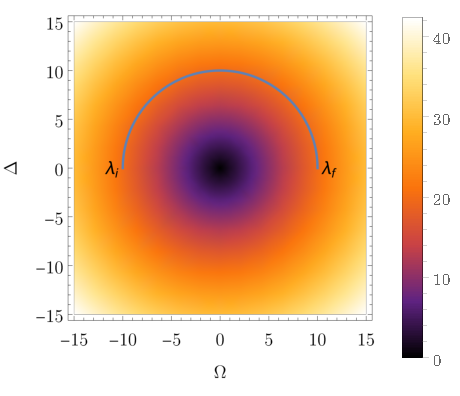
\includegraphics[scale=1.2]{../img/driving.pdf}
    \caption{Driving along the geodesic. $\lambda_i\equiv (\Omega_i,\Delta_i)$ and $\lambda_f\equiv (\Omega_f,\Delta_f)$ are initial and final parameters respective. Density plot shows the difference between Hamiltonian eigenvalues.}
    \label{fig:driving}
\end{figure}

\subsection{Derivation of the fidelity}
Because the Hamiltonian can be rewritten using Pauli matrices
\begin{equation}
    \HH(t) = 
        \begin{pmatrix}
         -s \cos (t \omega ) & s \sin (t \omega ) \\
         s \sin (t \omega ) & s \cos (t \omega ) \\
        \end{pmatrix}
        =\Delta(t)\sigma_x+ \Omega(t)\sigma_z= d(t).\mathbf{\hat{\bm\sigma}},
\end{equation}
for vector $\hat{\bm\sigma}\coloneqq (\hat\sigma_1,\hat\sigma_2,\hat\sigma_3)^T$.

One can see that changing from the \redd{original frame} with function $\ket{\psi}$ to \bluee{moving frame of reference}, with $\ket{\tilde\psi}$ (let's omit the final time dependence $\omega=\omega(T)$ for a while) is described as
\begin{equation}
    \redd{\psi(t)} \eqqcolon \expsp \bluee{\tilde\psi(t)}.
\end{equation}
This reflects the rotational symmetry of the system. The change of reference frame transforms Schr\"odinger equation as
\begin{equation}
    \begin{split}
        \redd{\HH(t)\psi(t)} &= i\redd{\psi'(t)}\\
        \redd{\HH(t)} \expsp\bluee{\tilde\psi(t)} &= i \expsp \left(\frac{i\omega\hat\sigma_y}{2}\right)\bluee{\tilde\psi(t)}+i\expsp\bluee{\tilde\psi'(t)}\\
        \underbrace{\left(\expsm \redd{\HH(t)}\expsp+ \frac{\omega}{2}\hat\sigma_y\right)}_{\bluee{\tilde H(t)}}\bluee{\tilde\psi(t)}&=i\bluee{\tilde\psi'(t)}.
    \end{split}
\end{equation}
One can equivalently solve the Fidelity problem in this new coordinate system.

Hamiltonian in the moving frame is
\begin{equation}
    \bluee{\tilde H}=\bluee{\begin{pmatrix}
        -s&-i\omega(T)/2\\
        i\omega(T)/2&s
    \end{pmatrix}},
\end{equation}
which is time independent and depends only on final time. The Schr\"odinger equation can now be easily solved using evolution operator
\begin{equation}
    \begin{split}
        \bluee{\UU(t)}=&e^{-i\bluee{\tilde H}t}
        =\bluee{\begin{pmatrix}
            \cos \left(\frac{t}{2} q\right)+\frac{2 i s \sin \left(\frac{t}{2} q\right)}{q} & -\frac{\omega  \sin \left(\frac{t}{2} q\right)}{q} \\
            \frac{\omega  \sin \left(\frac{t}{2} q\right)}{q} & \cos \left(\frac{t}{2} q\right)-\frac{2 i s \sin \left(\frac{t}{2} q\right)}{q} \\
        \end{pmatrix}},
    \end{split}
    \label{eq:evolutionBlue}
\end{equation}
for $q\coloneqq\sqrt{4 s^2+\omega(T) ^2}$.

In the original frame we get the evolution of $\psi(0)$ as
\begin{equation}
    \redd{\psi(t)}=\expsp \bluee{\UU(t) \tilde\psi(0)} = \underbrace{\expsp \bluee{\UU}\expsm}_{\redd{\UU(t)}} \underbrace{\expsp \bluee{\tilde\psi(0)}}_{\redd{\psi(0)}}.
\end{equation}
The evolved wave-function the reads as
\begin{equation}
    \redd{\ket{\psi(t)}}=\redd{\begin{pmatrix}
        \cos \left(\frac{t}{2} q\right)+\frac{2 i s}{q} \cos (t \omega ) \sin \left(\frac{t}{2} q\right)\\
        \frac{\omega -2 i s\sin (t \omega )}{q}  \sin \left(\frac{t}{2} q\right)
    \end{pmatrix}}
\end{equation}
and the ground state
\begin{equation}
    \redd{\ket{0(t)}}=\redd{\mathcal{N}\begin{pmatrix}
        -\cot (\frac{t}{2}\omega)\\
        1
    \end{pmatrix}},
\end{equation}
for a normalization constant $\redd{\mathcal{N}}\coloneqq |\redd{\braket{0(t)|0(t)}}|^{-1}$.
Fidelity during the transport is then\footnote{If we calculate the fidelity in the \bluee{comoving frame}, we get exactly one. This realization leads to the counter-diabatic driving.}
\begin{equation}
    F=\left|\redd{\braket{0(t)|\psi(t)}}\right|^2.
    \label{fid:definition}
\end{equation}

An explicit formula for fidelity in time $t$ and geodesic driving with final time $T$ is finally
\begin{equation}
    F(t,T)=\frac{\pi ^2 \left(\cos \left(t \sqrt{\frac{\pi ^2}{T^2}+4 s^2}\right)+1\right)+8 s^2 T^2}{2 \sin ^4\left(\frac{\pi  t}{2 T}\right) \left(4 s^2 T^2+\pi ^2\right) \left(\left| \cot \left(\frac{\pi  t}{2 T}\right)\right|^2+1\right)^2}.
    \label{eq:fidelitySimplified}
\end{equation}
The domain can be extended from $t\in(0,T)$ to $[0,T]$ for any $T\in[0,\infty]$, because 
$$
    \lim_{t\rightarrow 0}F=1\; ,\;\; \lim_{T\rightarrow 0}F=0.
$$

It is practical to define \emph{Infidelity} as
\begin{equation}
    F^*\coloneqq 1-F.
\end{equation} 
It has a meaning of \emph{excitation probability during the transport}.


\subsection{Analysis of the infidelity formula}
Infidelity can be calculated by numerical evolution of Schr\"odinger equation, or from Eq. \ref{eq:fidelitySimplified}. Sometimes both solutions are plotted for comparison between numerical precision. 

For some fixed final time, the infidelity is an oscillating curve with values close to $0$, see the driving for final time $T=1$ on Fig. \ref{fig:infidelityTimePlot}. The \emph{final infidelity} (fidelity at $t=T$) dependence on final time $T$ can be seen on Fig. \ref{fig:infidelityTfPlot} and \ref{fig:infidelityTfPlotLog}.
\begin{figure}[H]
    \centering
    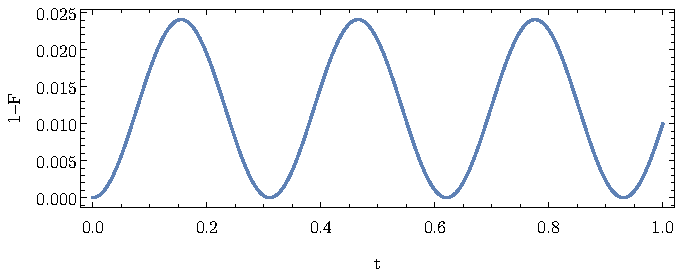
\includegraphics[scale=1.2]{../img/infidelityTimePlotGeod.pdf}
    \caption{Infidelity in time for final time $T=1$ for geodesical driving.}
  \label{fig:infidelityTimePlot}
\end{figure}

\vspace{-10pt}\begin{figure}[H]
    \centering
    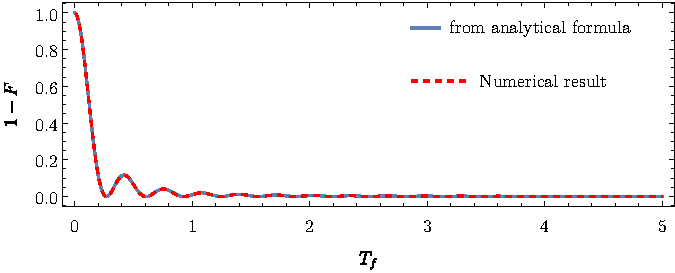
\includegraphics[scale=1.2]{../img/infidelityTfPlot.pdf}
    \caption{Final infidelity dependence on final time $T$ for geodesical driving.}
    \label{fig:infidelityTfPlot}
\end{figure}

\begin{figure}[H]
    \centering
    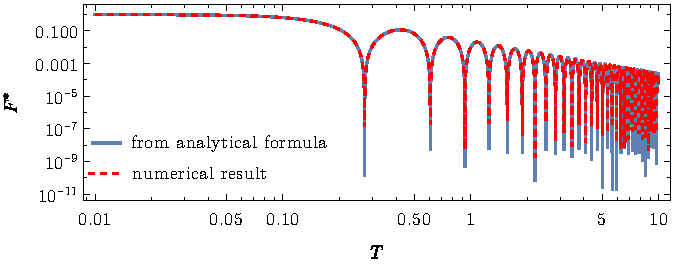
\includegraphics[scale=1.2]{../img/infidelityTfPlotLog.pdf}
    \caption{Final infidelity dependence on final time $T$ for geodesical driving; in logarithmic scale9. The difference in numerical precision of both methods can be seen in the spikes height. As it will be shown later, the spikes should go to zero, thus analytical formula has higher numerical precision.}
    \label{fig:infidelityTfPlotLog}
\end{figure}



From the fidelity formula \ref{eq:fidelitySimplified} goes that condition $F=1$ is equivalent to
\begin{equation}
    \cos \left(\sqrt{T_s^2+\pi ^2}\right)=1,
\end{equation}
for $T_s\coloneqq 2s T$. The solution to this equation is
\begin{equation}
    T_s=\sqrt{(2 \pi  k)^2-\pi ^2} \text{  for }k\in \mathbb{N},
    \label{eq:solutionT}
\end{equation}
see Fig. \ref{fig:fidelityZeros}. This implies that spikes on Fig. \ref{fig:infidelityTfPlotLog} have minimal value $1-F=0$, and their density is linear in $T$.
\begin{figure}[H]
    \centering
    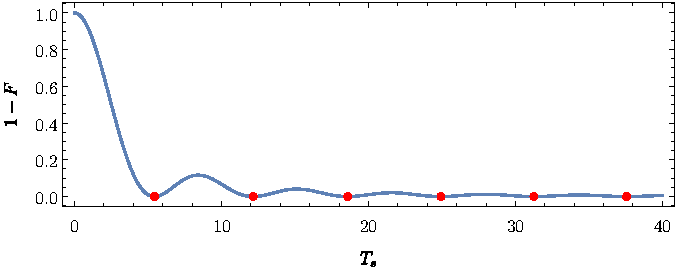
\includegraphics[scale=1.2]{../img/fidelityZeros.pdf}
    \caption{Rescaled final infidelity $T_s\coloneqq 2s T$ dependence on final time. Red points mark the condition $F=1$.}
    \label{fig:fidelityZeros}
\end{figure}


Fidelity as a function of time and final time can be seen in Fig. \ref{fig:dens3}. Note that only $t<T$ has physical meaning.

\begin{figure}[H]
    \centering
    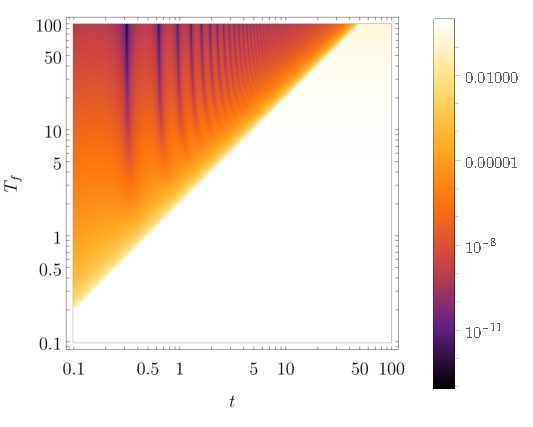
\includegraphics[scale=1.2]{../img/dens3.pdf}
    \caption{Fidelity dependence on time and final time in log-log scale. Only $t<T$ has a physical meaning.}
    \label{fig:dens3}
\end{figure}

\subsection{Energy variance}
Another interesting quantity is the energy variance, specially because of Theorem \ref{thm:polkovnikov}. Evaluating the fidelity for geodesical driving gives a function of time $t$ and final time $T$
\begin{equation}
    \begin{split}        
        \delta E^2 =& \frac{s^2}{2 q^2}\Bigg[\Big[16 s^4+2 s^2 \left(\left(\omega ^2-8 s^2\right) \cos (2 t \omega )-8 \omega ^2 \cos ^2(t \omega ) \cos \left(t \sqrt{q}\right)\right)\\
        &+14 s^2 \omega ^2+\omega ^4\Big] -\omega ^2 \left(\left(2 s^2+\omega ^2\right) \cos (2 t \omega )-2 s^2\right) \cos \left(2 t q\right)\\
        & +8 s^2 \omega  q \sin (2 t \omega ) \sin \left(t q\right) + \omega ^3 q \sin (2 t \omega ) \sin \left(2 t q\right) \Bigg],
\end{split}
\end{equation}
see the definition of $q$ under Eq. \ref{eq:evolutionBlue}. The result of energy variance can be seen on Fig. \ref{fig:densVar}. Note that only $t<T$ has a physical meaning, therefore the dependence is smooth along the whole geodesical driving protocols.

\begin{figure}[H]
    \centering
    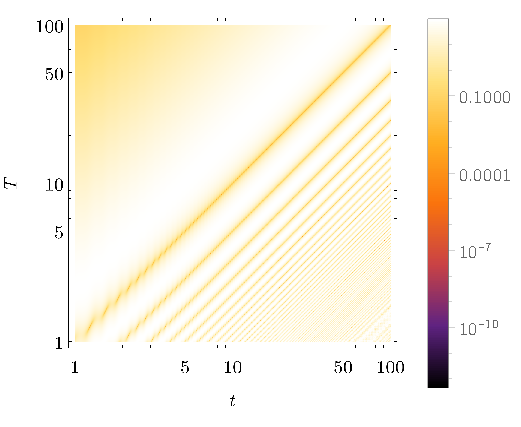
\includegraphics[scale=1.2]{../img/densVar.pdf}
    \caption{Energy variance for geodesical driving protocol, dependent on time $t$ and final time $T$. Driving occurs only in area $t<T$.}
    \label{fig:densVar}
\end{figure}

\newpage 
\section{Linear driving}
Another analytically solvable driving is defined using two scaling parameters $\Omega_{sc},\;\Delta_{sc}$, as 
\begin{equation}
    \Omega(t)=\Omega_{sc}\left(\frac{2t}{T}-1\right),\quad \Delta(t)=\Delta_{sc}, \;\;\text{ for } \Omega_{sc}=10, \Delta_{sc}=1,
    \label{eq:linearDrivingdef}
\end{equation}
see Fig. \ref{fig:driving1}. 
\begin{figure}[H]
    \centering
    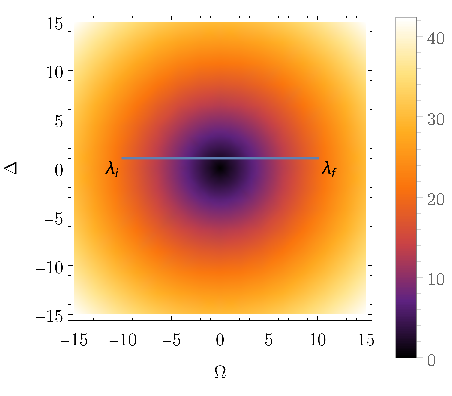
\includegraphics[scale=1.2]{../img/drivingLin.pdf}
    \caption{Driving along the linear path. $\lambda_i\coloneqq(-10;1)$ and $\lambda_f\coloneqq(10;1)$ are initial and final parameters respective. Density plot shows the difference between Hamiltonian eigenvalues.}
    \label{fig:driving1}
\end{figure}

From linear driving definition \ref{eq:linearDrivingdef} and energy dependence \ref{eq:energy} we have
\begin{equation}
    \dot \Delta(t)=0;\quad \Delta(t) \overset{\textcolor{gray}{\Delta(t)>0}}{=} \sqrt{\frac{E^2_{dif}(t)}{4}-\Omega^2(t)};\quad E_{dif}\coloneqq E_1-E_0.
\end{equation}
Substituting to Harmonic oscillator damping and frequency functions (Eq. \ref{eq:gammaDef} and \ref{eq:frequency}) we get 
\begin{align}
    \gamma(t) &= 0\\
    \omega^2(t)&=i\frac{2\Omega_{sc}}{T}+\frac{\Omega_{sc}}{4}\left(\frac{2t}{T}-1\right)^2+\frac{\Delta_{sc}^2}{4}=i\frac{2\Omega_{sc}}{T}+\frac{E^2_{dif}(t)}{4}.
    \label{eq:oscillationsLinear}
\end{align}
Corresponding differential equation of second order is
\begin{equation}
    a''(t)+\omega^2(t) a(t)=0,
\end{equation}
which is of \emph{Weber type}\footnote{https://mathworld.wolfram.com/WeberDifferentialEquations.html} with Parabolic Cylinder functions\footnote{https://mathworld.wolfram.com/ParabolicCylinderFunction.html} as a solution, see \citet{felipe}. 

\subsection{Dependence on time}
The fidelity in time can be seen on Fig. \ref{fig:infidelityTimePlotLin}. For $t\approx T/2$, the difference between energy levels is minimal, which leads to fast state excitation. Then the Harmonic oscillator damping gets involved, and oscillations quickly go to zero, never disappearing entirely.

We can see that the final fidelity decreases with a longer final time, which correctly leads to adiabatic driving, where $\lim_{T\rightarrow \infty} F^*=0$. For short final times we can observe so-called quench, $\lim_{T\rightarrow 0} F^*=1$. The interesting phenomena in this image are the oscillations around $t=T/2$, for which the frequency increases with a longer final time. 

\begin{figure}[H]
    \centering 
    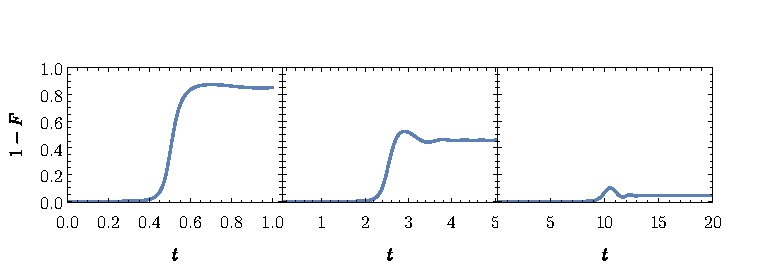
\includegraphics[scale=1.185]{../img/infidelityInTimePlot1.pdf}
    \caption{Infidelity in time for three final times $T\in\{1,5,20\}$ for the linear driving defined in \ref{eq:linearDrivingdef}.}
  \label{fig:infidelityTimePlotLin}
\end{figure}


Because in the Harmonic oscillator $\gamma(t)=0$, the oscillations of $a(t)$ are not damped. What we are observing is infidelity 
$$F^*(t)\coloneqq 1- |\braket{0(t)|\psi(t)}|^2 = 1-|\alpha(t)a(t)+\beta(t)b(t)|^2, $$
where the $\ket{\psi(t)}\eqqcolon(a,b)^T$ represents the evolved state and $\ket{0(t)}\eqqcolon(\alpha,\beta)^T$ evolved ground state in fixed eigenbasis $\mathcal{B}$. The ground state is not generally constant. In our case, the ground state described by Eq. \ref{eq:eigenvectors} and is slowly changing its value from the first element $\alpha$ to the second element $\beta$, see Fig. \ref{fig:zeroState}. This means that at the beginning of driving, the projection to the ground state selects $b(t)$. Then it's getting more influenced by $a(t)$ until almost only $a(t)$ influences the fidelity.
\begin{figure}[H]
    \centering
    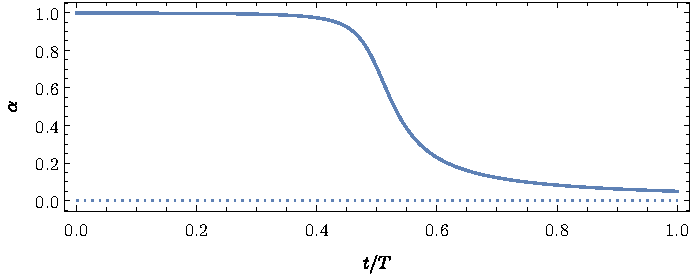
\includegraphics[scale=1.2]{../img/zeroState.pdf}
    \caption{Value of first element of the ground state vector $\alpha\equiv \ket{0(t)}^1$ during linear driving.}
    \label{fig:zeroState}
\end{figure}

Because of varying ground state during transport, the oscillations cannot be analyzed only from $\omega^2(t)$ described by Eq. \ref{eq:oscillationsLinear}. At the end of the driving we have 
\begin{equation}
   \frac{1}{N_+} \ket{0(t)}^1=\frac{E_0(t)+\Omega(t)}{\Delta(t)}\gg 1 =\frac{1}{N_+} \ket{0(t)}^2,
\end{equation}
leading to the \emph{fidelity at the end of the driving}
\begin{equation}
    F_{end}= \left|N_+ \left(
        \frac{E_0(t)+\Omega(t)}{\Delta(t)} a(t)+b(t)
        \right)\right|^2 \approx b^2(t),
\end{equation}
therefore when $t$ is getting close to $T$ the fidelity is oscillating with  harmonic oscillator frequency \ref{eq:frequency}.




\subsection{Final fidelity}
Because the oscillations after fast parameter change in the Hamiltonian never disappear entirely, we must observe these oscillations even at the final time. \emph{Final fidelity} (meaning the fidelity at $t=T$) has dependence on $T$ as can be seen in Fig. \ref{fig:infidelityTfPlotLogLinCombined}. Because after the final time $T\approx 120$, the values are small enough to observe some fine structure of the fidelity along with numerical error artifacts.
\begin{figure}[H]
    \centering
    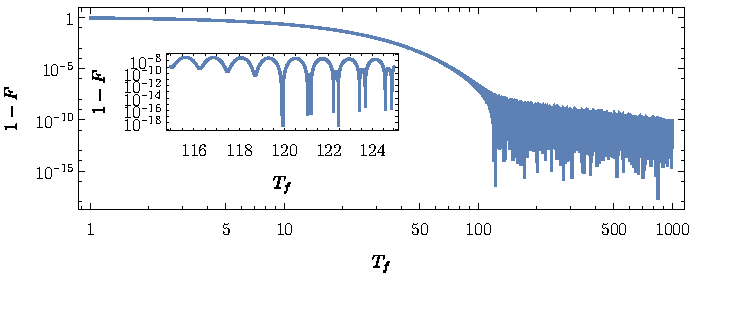
\includegraphics[scale=1.2]{../img/infidelityTfPlotLogLinCombined1.pdf}
    \caption{Final infidelity as a function of $T$ with zoom on the transitional part.}
    \label{fig:infidelityTfPlotLogLinCombined}
\end{figure}

First, the numerical precision of this calculation was found to be around $10^{-13}$. This means that the oscillations we see in Fig. \ref{fig:infidelityTfPlotLogLinCombined} are of physical origin with some additional numerical error. These small oscillations are the remnants of the fast excitation during the close approach of energy levels, see Fig. \ref{fig:infidelityTimePlotLin}. The reason is that the choice $t=T$ sometimes corresponds to the oscillation minima and sometimes to its maxima.



\subsubsection{Averaged final fidelity}
We can eliminate the effect of oscillations by averaging over time. For that we define the \emph{average final infidelity}
\begin{equation}
    \langle F^*\rangle_p(T) \coloneqq \frac{1}{(1-p) T}\int\limits_{p T}^{T} F^*(t)\d t.
\end{equation}
It turned out that averaging over 1 \% ($p=0.99$) or 10 \% ($p=0.9$) of the driving gave approximately the same results for long enough drivings ($T\overset{\sim}{>} 10$). The same result can be obtained from the analytical continuation of the fidelity formula to $t\rightarrow  \infty$. This analytical continuation of the harmonic oscillator solution leads to the Fidelity value around which the oscillations occur. The result of averaging can be seen in Fig. \ref{fig:infidCombined}.

Using this we can describe the driving using three regimes\footnote{The coefficient $p$ is assumed to be small enough not to cover the biggest oscillations after $t=T/2$ and big enough to average over sufficient number of oscillations. Approximately $p\in[0.6T,0.999T]$.}.
\begin{itemize}
    \item \emph{Exponential/fast-driving regime} — $\langle F^*\rangle_p= \exp(-\xi T)$, $\xi\in\R^+$
    \item \emph{transitional regime} — happens around \emph{critical time} $T_c$.
    \item \emph{Polynomial/close-adiabatic regime} — $\langle F^*\rangle_p\propto T^{-\kappa}$ for $\kappa\in \R^+$.
\end{itemize}

\begin{figure}[H]
    \centering
    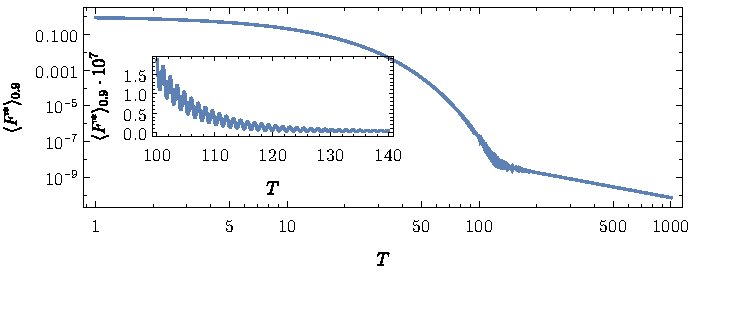
\includegraphics[scale=1.2]{../img/infidCombined1.pdf}
    \caption{Final infidelity as a function of $T$ in log-log scale wit linear scaled plot inserted.}
    \label{fig:infidCombined}
\end{figure}



The boundary between exponential and linear regime is not strict and can be seen on Fig. \ref{fig:dens2}, as transition between \emph{smooth} and \emph{chaotic} regimes. This happens around $t=T_c$. The fine structure, see Fig. \ref{fig:dens2Zoom}, is caused by the oscillatory character of the final fidelity. This can be< smoothed out using the averaged final fidelity. The approximated dependence for final time was numerically estimated as
\begin{equation}
    T_c\overset{\sim}{\propto} \Delta_{sc}^{-2}.
\end{equation}


\begin{figure}[H]
    \centering 
    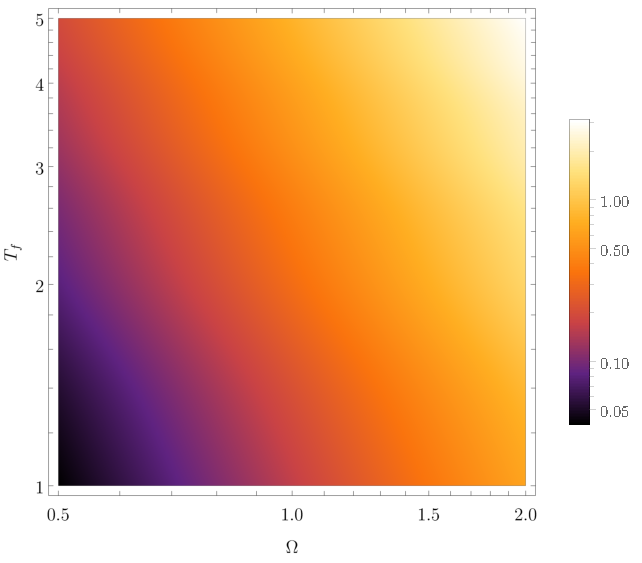
\includegraphics[scale=1.2]{../img/dens2.pdf}
    \caption{Final infidelity as a function of $\Delta$ and $T$ and its three regimes. Zoom on the boundary between them can be seen on \ref{fig:dens2Zoom}.}
    \label{fig:dens2}
\end{figure}

\vspace{-10pt}\begin{figure}[H]
    \centering 
    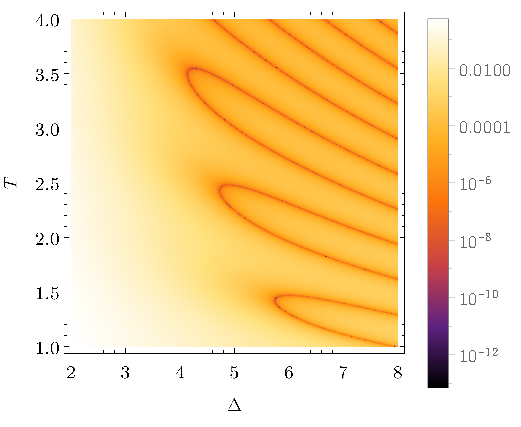
\includegraphics[scale=1.2]{../img/dens2Zoom.pdf}
    \caption{Fine structure of the boundary between fast-driving and adiabatic regimes of final infidelity.}
    \label{fig:dens2Zoom}
\end{figure}



To understand the infidelity oscillations, compare Fig. \ref{fig:undercritical} with \ref{fig:overcritical}. Here we see two regimes, one for $t<T_c$ and one for $T>T_c$. The important observation is that in the first case, $F^*\neq 0$ for all $t>0$, and in the second case, it touches zero periodically. The fidelity can be decomposed into a sum of two elements. The small oscillatory part, which the theory of APT can explain, and exponentially decreasing fidelity with final time, is described by the Landau-Zener formula.

\begin{figure}[H]
    \centering
    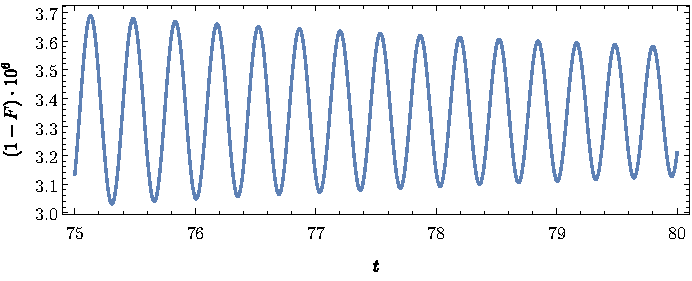
\includegraphics[scale=1.2]{../img/undercritical.pdf}
    \caption{Infidelity as a function of time for fast-driving regime, $T=80<T_c$.}
    \label{fig:undercritical}
\end{figure}

\begin{figure}[H]
    \centering
    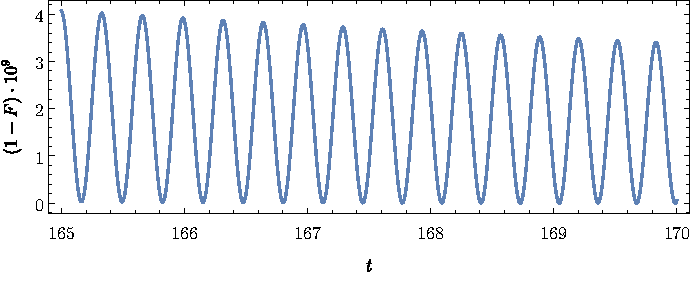
\includegraphics[scale=1.2]{../img/overcritical.pdf}
    \caption{Infidelity as a function of time for close-adiabatic regime. $T=170>T_c$}
    \label{fig:overcritical}
\end{figure}

\subsubsection{Exponential and polynomial part, Landau-Zener and APT}
Landau-Zener-Stueckelberg's theory provides the WKB approximation formula for the fidelity during some transport. The complete form can be seen in the book by \citet{nonadiabaticTransition}. In this case, only a simplified theorem is needed. First, let's review some definitions.

\begin{definition}[Diabatic coupling]
    Diabatic coupling functions are off-diagonal elements of two-level Hamiltonian. At avoided crossing, it is half of Hamiltonian eigenvalue difference,
    \begin{equation}
        A=\frac{E_2-E_1}{2}.
    \end{equation}
\end{definition}
\begin{definition}[Diabatic potential]
    Difference between Hamiltonian eigenvalues can be linearly approximated as
    \begin{equation}
        \Delta E\equiv E_1-E_0 \eqqcolon \alpha t
    \end{equation}
    Diabatic potential difference is the ratio
    \begin{equation}
        |\Delta F|\coloneqq \left|\frac{\alpha}{t}\right|.
    \end{equation}
\end{definition}

\begin{thm}[Landau-Zener-Stueckelberg (LZS) for linear driving]
    For 
    \begin{itemize}
        \item two level Hamiltonian
        \item with degeneracy in only one point,
        \item on the linear driving path in a parametric space,
    \end{itemize}
    the fidelity can be described for times $t\in(0,T_c)$ as
    \begin{equation}
        F = \exp\left(-\frac{2 \pi A^2}{v|\Delta F|}\right),
        \label{eq:exponentialPart}
    \end{equation}
    for a \emph{diabatic coupling} $A$, and \emph{diabatic potential difference} $|\Delta F|$. 
\end{thm}

In our case, the speed $v=1/T$ is constant, off-diagonal elements are also constant $A=\Delta_{sc}$, and the driving path is symmetric along $\Omega=0$ axis, leading to $|\Delta F|=2\Omega_i$.

The polynomial, or chaotic regime, can be explained using APT. It holds that
\begin{equation}
    \log(F^*)=\log(T^{-2})+\log\left(\sum_{i=1}^n |b_n^{(1)}(T)|^2\right),
    \label{eq:polynomialPart}
\end{equation}
for functions $b_n^{(1)}$ from Eq. \ref{eq:bnAPT}. For more details, see \citet{felipe}.

The LZS approximation can be seen in Fig. \ref{fig:landauCompare}. The LZS and APT approximations give the leading order in corresponding regimes (omitting the oscillations) and intersect at time $T_c$. These two parts are not only a good approximation on both intervals, but if added together, they represent the whole fidelity curve with very high precision. Adding these two solutions together might not give a good mathematical meaning. It can be done because the APT gives the infidelity of order $10^{-9}$, it creates a negligible error. The advantage is that one gets a suitable approximation for the transitional regime with this process.


\begin{figure}[H]
    \centering 
    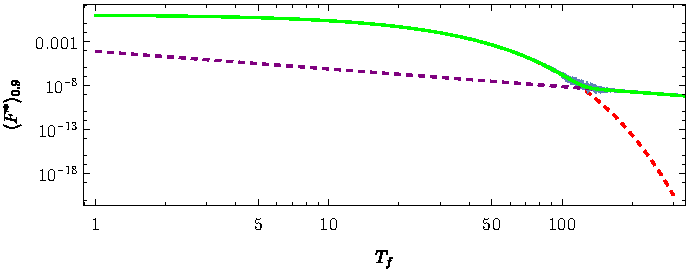
\includegraphics[scale=1.2]{../img/landauCompare.pdf}
    \caption{Fidelity as a function of driving final time, approximated by the \green{sum (green)} of \red{Landau-Zener (red, dashed)} and \textcolor{purple}{APT (purple, dashed)}}
    \label{fig:landauCompare}
\end{figure}
% \subsection{Multiparametric behavior}
% The critical time $T_c$ is the point where the fidelity dependence on final time becomes polynomial. We have shown that 
% \begin{equation}
%     \text{for}\begin{cases}
%         T<T_c \\
%         T>T_c 
%     \end{cases}\text{the fidelity oscillate with amplitude } A \text{ is }
%     \begin{cases}
%         A<1-F_{final}\\
%         A>1-F_{final}
%     \end{cases}.
% \end{equation}

\subsection{Summary of linear driving}
Now that we understand all results separately let's put it all together. In Fig. \ref{fig:AllInOne} the most important results can be seen. The difference between the close adiabatic regime and the fast regime at the end of the driving is if $F^*=0$. The chaotic regime is below $t=T$ line for $T<T_c$ and the chaotic cone is crossing this line around $t=T_c$.

\begin{figure}[H]
    \centering 
    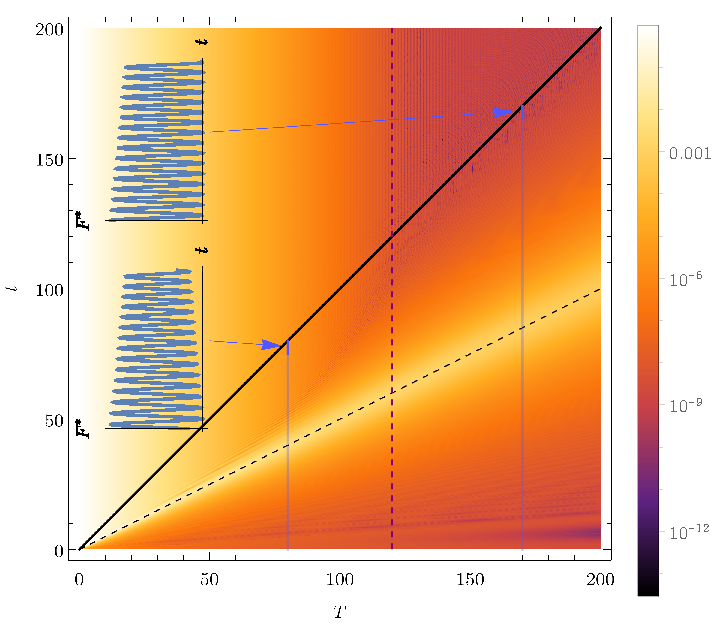
\includegraphics[scale=1.2]{../img/allInOne.pdf}
    \caption{Fidelity dependence for linear driving with $\Delta=1$. Black line marks $t=T$, dashed black line $t=T/2$ and \redd{purple} dashed line is the approximate value of $T_c$. \bluee{Blue} lines marks driving from Fig. \ref{fig:undercritical}, \ref{fig:overcritical}, visualizing the final times of the driving.}
    \label{fig:AllInOne}
\end{figure}


\newpage
\subsection{Energy variance}
Analogically to the geodesical driving, one might be interested in energy variance. In the linear driving case, the analytical formula is more complicated and only numerical result are displayed here. On Fig. \ref{fig:densVariance} the energy variance is plotted as a function of time and final time.
\begin{figure}[H]
    \centering
    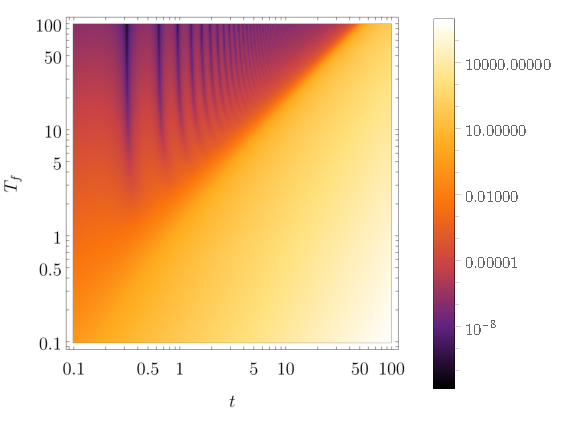
\includegraphics[scale=1.2]{../img/densVariance.pdf}
    \caption{Energy variance for $\Delta_{sc}=0.2$ for linear driving. Note that only $t<T$ has physical meaning.}
    \label{fig:densVariance}
\end{figure}
\chapter{Lipkin-Meshkov-Glick model}
\label{chap:lipkin}

The Lipkin-Meshkov-Glick (LMG) model is a simple model manifesting the quantum phase transitions. It represents a many-body fermion system. This chapter aims to understand the properties of the ground state and its influence on different driving protocols.


The model is defined on a parametric space $\llambda\equiv (\lambda;\chi)\in\mathcal U\coloneqq \R^2$ with Hamiltonian
\begin{equation}
    \HH(\lambda,\chi)=\J_3+\lambda\hat V_1 +\chi \hat V_2+\chi^2 \hat V_3,
    \label{eq:firstOrderTransitionHamiltonian}
\end{equation}
where
\begin{align}
    \hat V_1 &\coloneqq-\frac{1}{2j}\J_1^2\\
    \hat V_2 &\coloneqq -\frac{1}{2j}\left[\J_1(\J_3+j\Id)+(\J_3+j\Id)\J_1\right]\\
    \hat V_3 &\coloneqq -\frac{1}{2j}(\J_3+j\Id)^2
\end{align}
and \emph{angular momentum operator} $\bm\J=(\J_1,\J_2,\J_3)^T$.

Using the Spherical harmonics\footnote{https://mathworld.wolfram.com/SphericalHarmonic.html} basis $\{\ket{j,m}\}$ for quantum numbers $j$ as the angular momentum and $m$ its projection to the direction of $\J_3$ and defining
\begin{equation}
    \J_\pm\coloneqq\frac{1}{2}(\J_1\pm i\J_2),
\end{equation}
we get matrix elements
\begin{align}
    \braket{j'm'|\J^2|jm} &= j(j+1)\delta_{j'j}\delta_{m'm}\\
    \braket{j'm'|\J_3|jm} &= m \delta_{j'j}\delta_{m'm}\\
    \braket{j'm'|\J_\pm|jm} &= \sqrt{(j\mp m)(j\pm m+1)}\delta_{j'j}\delta_{m'm\pm 1},
\end{align}
where $\delta_{a'b}$ is Kronecker delta. The Hamiltonian in Eq. \ref{eq:firstOrderTransitionHamiltonian} can then be written as
\begin{equation}
\begin{split}
        % \left(\J_1+\chi(\J_3+j)\right)^2 &= \textcolor{purple}{\J_1^2} +\chi^2 (\J_3^2+j^2\Id+2j\J_3)+\chi(\textcolor{blue}{\J_1}\J_3+\J_3\textcolor{blue}{\J_1})+2\chi j\textcolor{blue}{\J_1}\\
        % \textcolor{purple}{\J_1^2}&= \frac{1}{4}(\J_++\J_-)^2= \frac{1}{4}(\J_+^2+\J_-^2+\textcolor{violet}{\J_+\J_-}+\textcolor{violet}{\J_-\J_+})\\ 
        % \textcolor{violet}{\J_\pm\J_\mp}&=\J^2-\J_3^2 \mp \J_3\\
        % \textcolor{blue}{\J_1}&=(\J_+ +\J_-),\\
        \HH =& J_3-\frac{\lambda}{8j}(J_++J_-)^2-\frac{\chi}{4j}\left[(J_++J_-)(J_3+j\Id)+(J_3+j\Id)(J_++J_-)\right]\\
        &-\frac{\chi^2}{2j}(J_3+j\Id)^2,
\end{split}
\end{equation}
which has pentadiagonal matrix representation. During the whole chapter, $j=N/2$ is used. 

First, the low dimensional cases of this Hamiltonian are analyzed, especially $N=3$, where the analytical formula for energy spectrum can be found. The limit $N\rightarrow \infty$ is then taken, showing the correspondence to the classical system. Finally, some generalization to an arbitrary dimension and an example of transport using quenches is presented. 











\section{Geometry for fixed dimension}
Because of a penta-diagonal form of the Hamiltonian, the discussion starts at $N=3$, followed by $N=5$ and $N\rightarrow\infty$.

Due to the complexity of our Hamiltonian, it is not possible to prove every statement analytically. Some numerical methods, supported by mathematical theorems, are therefore used.



\subsection{3-dimensional Hamiltonian}
The lowest dimension behaving similarly to higher $N$ is 3. The matrix represented Hamiltonian is
\begin{equation}
    \HH=\left(
        \begin{array}{cccc}
         -\frac{ \lambda +6}{4} & -\frac{\chi }{2 \sqrt{3}} & -\frac{\lambda }{2 \sqrt{3}} & 0 \\
         -\frac{\chi }{2 \sqrt{3}} & \frac{ \left(-7 \lambda -4 \chi ^2-6\right)}{12} & -\chi  & -\frac{\lambda }{2 \sqrt{3}} \\
         -\frac{\lambda }{2 \sqrt{3}} & -\chi  & \frac{ \left(-7 \lambda -16 \chi ^2+6\right)}{12} & -\frac{5 \chi }{2 \sqrt{3}} \\
         0 & -\frac{\lambda }{2 \sqrt{3}} & -\frac{5 \chi }{2 \sqrt{3}} & -\frac{\lambda }{4}-3 \chi ^2+\frac{3}{2} \\
        \end{array}
        \right).
\end{equation}
The spectrum of this Hamiltonian can be calculated analytically using some complex functions $D, E, F, G:\C\rightarrow \C$, see Appendix \ref{appendix1}, as
\begin{align}
        E_0 &= \frac{1}{12} \left(G-F-\frac{\sqrt{D-E}}{2}\right)
        \label{eq:N=3_en0}\\
        E_1 &= \frac{1}{12}  \left(G-F+\frac{\sqrt{D-E}}{2}\right)
        \label{eq:N=3_en1}\\
        E_2 &= \frac{1}{12} \left(G+F-\frac{\sqrt{D+E}}{2}\right)
        \label{eq:N=3_en2}\\
        E_3 &= \frac{1}{12}  \left(G+F+\frac{\sqrt{D+E}}{2}\right).
        \label{eq:N=3_en3}
\end{align}
Eigenvectors can also be expressed analytically, but due to their complexity only analytical results are presented here. On sections $\lambda=1$ and $\chi=1$ (see energy spectrum on Figures \ref{fig:N=3_energiesl} and \ref{fig:N=3_energiesc} respective), the energies get close to each other somewhere around the center of our coordinate system $(\lambda;\chi)$ and then separate monotonously to never meet again. The spectrum has $\chi\leftrightarrow -\chi$ symmetry. These close approaches of energy levels are important, because of their influence on geometry of energy state manifolds.
\begin{figure}[h]
    \centering
    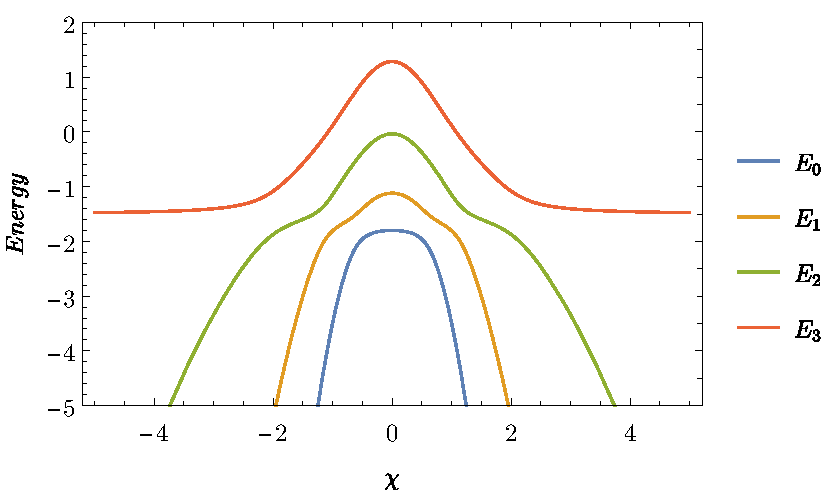
\includegraphics[scale=1.3]{../img/N=3_energiesl.pdf}
    \caption{Energy spectrum for $N=3$, section $\lambda=1$}
    \label{fig:N=3_energiesl}
\end{figure}
\begin{figure}[h]
    \centering
    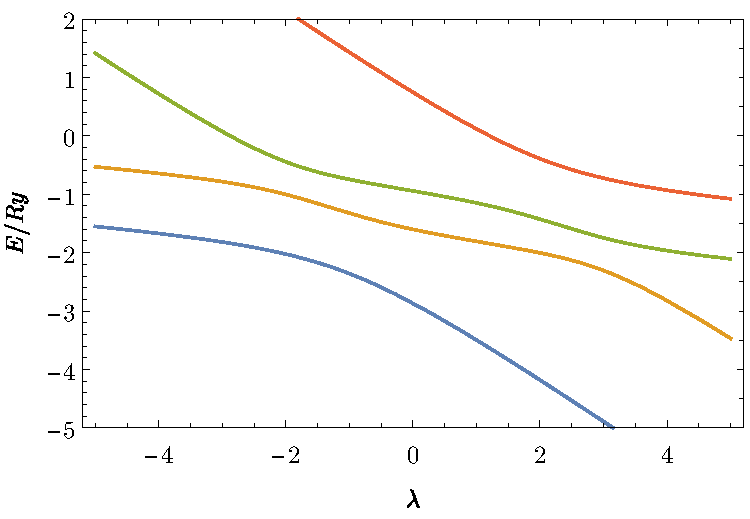
\includegraphics[scale=1.3]{../img/N=3_energiesc.pdf}
    \caption{Energy spectrum for $N=3$, section $\chi=1$}
    \label{fig:N=3_energiesc}
\end{figure}

From Eq. \ref{eq:N=3_en0}, \ref{eq:N=3_en1} can be seen the possible existence of spectrum degeneracies between every two neighboring energy levels\footnote{If the functions $D,E,F,G$ were into real numbers, degeneracies would exist between every two neighboring energy levels. Because they are complex, the solution $E_i=E_j$ might not exist. From numerical results, degeneracies exist between every two neighboring energy levels.}. Degeneracy $\bluee{E_0}=\textcolor{orange}{E_1}$ holds for $D=E$, which for real values $\lambda,\;\chi$ has two solutions
$$(\lambda_d,\pm \chi_d)=\left(-\frac{1}{2};\sqrt{\frac{3}{5}}\right).$$
According to Theorem \ref{thm:n-2}, Hamiltonian driven by two real parameters can be degenerated only on 0-dimensional manifolds. This means that degeneracies can be only separated points in the parametric space.

If the energy spectrum is degenerate and the metric tensor diverges, see individual elements in Fig. \ref{fig:N=3_g}, its determinant also diverges, as shown in Fig. \ref{fig:N=3_gDivenrgence}, along with Christoffel symbols in Fig. \ref{fig:N=3_G}. The metric tensor determinant is positive definite; therefore, the manifold is Riemannian. Further on, it reflects the symmetry $\chi\leftrightarrow-\chi$, except for elements $g_{12}$, $\Gamma_{121}$, $\Gamma_{211}$, and $\Gamma_{222}$, which switch their sign.

\begin{figure}[H]
    \centering
    \begin{tikzpicture}
        \node[] at (0,0) {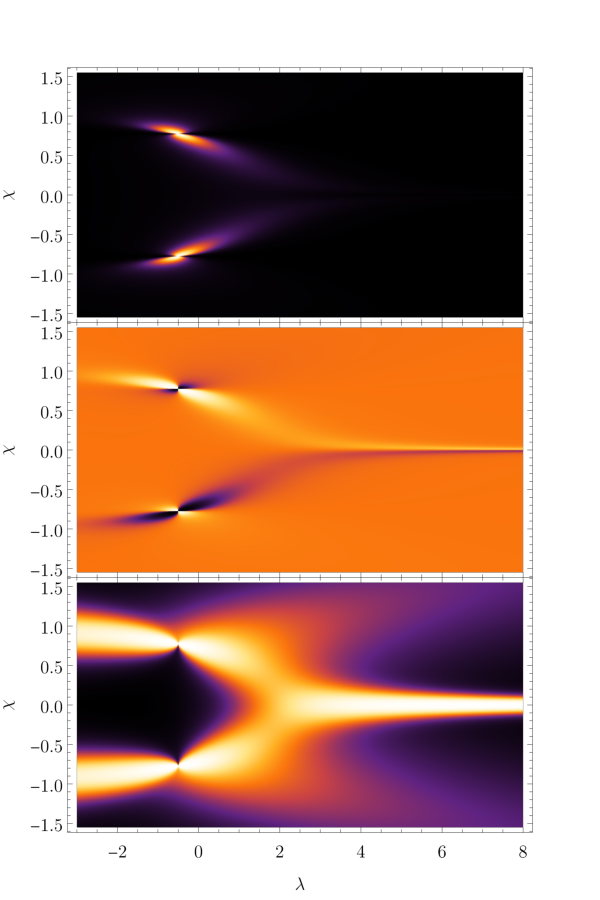
\includegraphics[scale=1.3]{../img/N=3_gComponents.pdf}};
        \node[] at (0,-11) {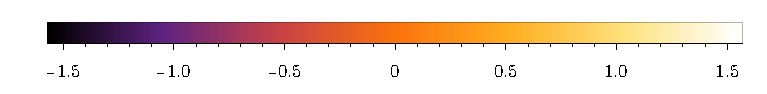
\includegraphics[scale=1.3]{../img/N=3_barA.pdf}};
        \node[] at (3.5,7.66) {\textcolor{white}{$\arctan(g_{11})$}};
        \node[] at (2.2,2.0) {\textcolor{white}{$\arctan(g_{12})=\arctan(g_{21})$}};
        \node[] at (3.5,-3.5) {\textcolor{white}{$\arctan(g_{22})$}};
    \end{tikzpicture}
\caption{Arctangent of the metric tensor elements for $N=3$ in the parametric space.}
    \label{fig:N=3_g}
\end{figure}

\begin{figure}[H]
    \centering
    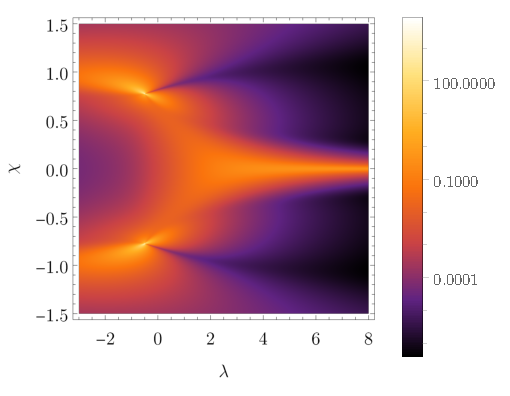
\includegraphics[scale=1.3]{../img/N=3_gDivergence.pdf}
    \caption{Ground state metric tensor determinant in a parametric space for $N=3$.}
    \label{fig:N=3_gDivenrgence}    
\end{figure}

\vspace{-30pt}
\begin{figure}[H]
    \centering
    \begin{tikzpicture}
        \node[] at (0,0) {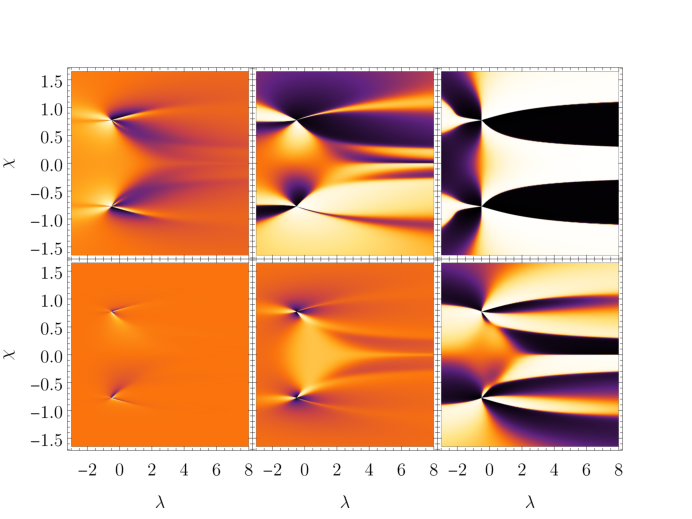
\includegraphics[scale=1.3]{../img/N=3_gammas.pdf}};
        \node[] at (-0.5,-6.5) {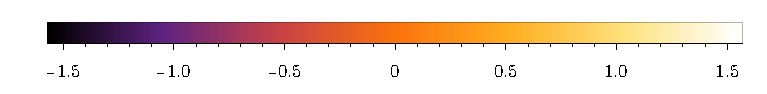
\includegraphics[scale=1.3]{../img/N=3_barA.pdf}};
        \node[] at (-3.4,0.5) {$\arctan(\Gamma_{111})$};
        \node[] at (0.7,0.5) {$\arctan(\Gamma_{121})$};
        \node[] at (4.75,0.5) {$\arctan(\Gamma_{122})$};
        \node[] at (-3.4,-0.5) {$\arctan(\Gamma_{211})$};
        \node[] at (0.7,-0.5) {$\arctan(\Gamma_{221})$};
        \node[] at (4.75,-0.5) {$\arctan(\Gamma_{222})$};
    \end{tikzpicture}
    \caption{Arctangent of the ground state Christoffel symbols for $N=3$.}
    \label{fig:N=3_G}
\end{figure}


Due to metric tensor degeneracy, the space is not geodesically maximal. To see that the singularity is not only \emph{coordinate one}\footnote{Coordinate singularity is present only in some coordinates. This is different from the so-called \emph{physical singularity}, which is present in every choice of the coordinate system.} the Ricci scalar can be calculated, see Fig. \ref{fig:N=3_Ricci}. Divergent Ricci scalar implies that singularity is physical. This can be seen from sections in $\chi$-direction drawn in Fig. \ref{fig:N=3_Ricci_section}, which at coordinate $(\lambda_d;\chi_d)$ diverges. The coordinate independence implies the singularity is \emph{physical}. 


\begin{figure}[H]
    \centering
    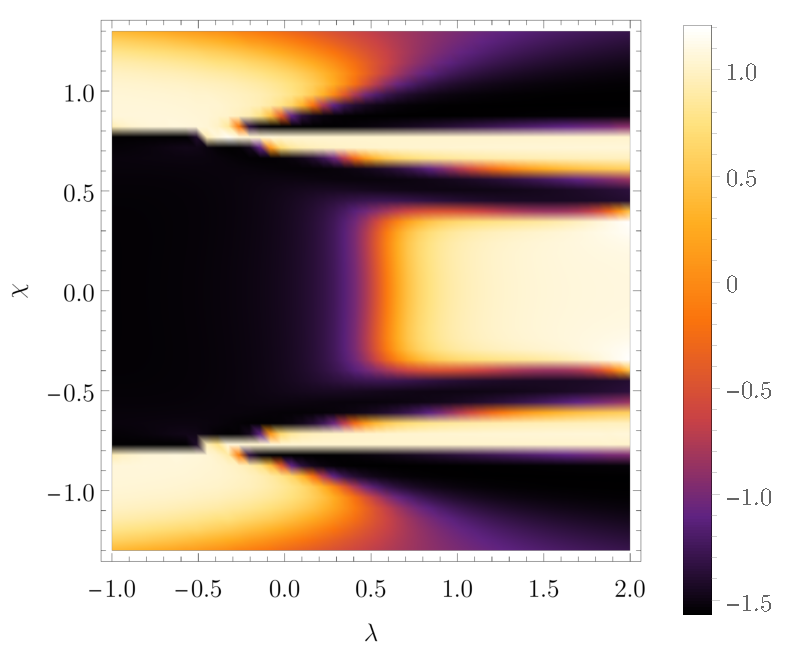
\includegraphics{../img/N=3_Ricci.pdf}
    \caption{Arctangent of Ricci curvature for the case $N=3$.}
    \label{fig:N=3_Ricci}
\end{figure}

% Coordinates of minima on lines with constant $\lambda$ in Ricci scalar can be seen in Fig. \ref{fig:N=3_RicMinimas} and will be important later on, because geodesics will be strongly repelled by parts of this line.
\begin{figure}[H]
    \centering
    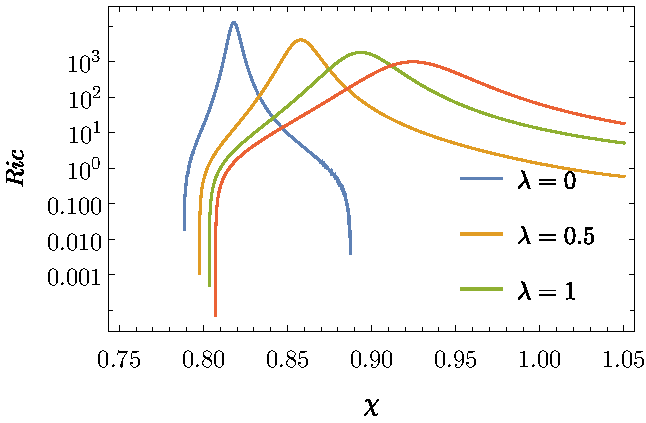
\includegraphics[scale=0.9]{../img/N=3_Ricci_section.pdf}
    \caption{Ricci curvature sections for three different $\lambda$. $N=3$.}
    \label{fig:N=3_Ricci_section}
\end{figure}
% \begin{figure}[H]
%     \centering
%     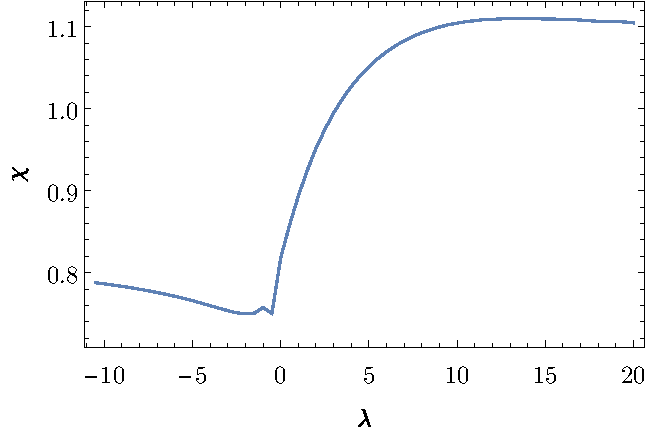
\includegraphics[scale=0.9]{../img/N=3_RicMinimas.pdf}
%     \caption{Minimas in Ricci curvature on the background of metric tensor determinant. Case $N=3$.}
%     \label{fig:N=3_RicMinimas}    
% \end{figure}


\subsubsection{Geodesics}
The importance of geodesics was described in Chapter \ref{chap:groundStateManifoldDriving}. In addition, they give a tool for observing some system characteristics, such as singularities, or curvature in general. \emph{Initial valued Geodesics} are solutions to
$$(\lambda(0);\chi(0))\eqqcolon (\lambda_i;\chi_i)$$
$$\left(\der{\lambda(t)}{t};\der{\chi(t)}{t}\right)\Bigg|_{t=0} \eqqcolon (\lambda'_i;\chi'_i),$$
where zero was set as initial time.

One might also choose \emph{boundary valued geodesics} with fixed initial $(\lambda(0);\chi(0))$ and final position $(\lambda(T);\chi(T))$. Because the shape of geodesics in parametric space does not depend on the initial derivative, it does not depend on the speed of driving in the parametric space. Initial valued geodesics are therefore more advantageous to calculate because they have only three free parameters — the initial coordinates $(\lambda_i;\chi_i)$ and ratio $\lambda'_i/\chi'_i$. Another reason is purely numeric, which is that boundary-valued geodesics are calculated by numerous evolutions of initial valued geodesics. Essentially the software evolves many initial valued geodesics and checks if the final boundary condition is satisfied. If not, the initial parameters are tweaked in response until it fits the boundary conditions. Calculating the boundary valued geodesics is generally much slower. In this case, the calculation time was $10$ to $100$ times longer.

Results for geodesics starting at $(\lambda_i;\chi_i)=(0;0)$, $
(\lambda',\chi')=(\cos\theta;\sin\theta)$ can be seen in Fig. \ref{fig:N=3_geodesics}. Other values $\theta$ result in a close approach of the geodesics to the singularity, making the calculation numerically unstable. The fact that geodesics lean toward singularities is well known from the theory of General Relativity (GR). The main difference here is that our "test particle" seems to be partially repulsed by the singularity. The analogy with GR then fails because of the nonexistence of negative mass and gravitational dipoles. The better analogy is electromagnetism, which has a downside in the fact that geometrical formalism is not used so much in this theory. A comparison of these two intuitive examples can be seen in Fig. \ref{fig:geodesicsinGR}. The geodesic behavior is caused not only by the singularity but also by a large Ricci curvature leaning to the right from it. This means the distance across this \emph{\blueee{unreachable gap}}, marked by \blueee{blue line} in Fig. \ref{fig:N=3_geodesics}, is also large. The geodesics then tend to go around this line rather than crossing it. The presence of singularities means that our ground state manifold is geodesically incomplete, and according to Theorem \ref{thm:hopf-Rinow_modified}, there exist some geodesically unreachable coordinates. From this goes the term \emph{\blueee{unreachable gap}}.

The fact that geodesics lean toward singularities and parts of parametric space with small energy level difference $\Delta E$ implies that for general fidelity driving, the geodesics cannot be advantageous in the case of fidelity. The excitation probability increases with smaller $\Delta E$ leading to a fidelity decrease for such drivings.


\begin{figure}[H]
    \centering
    % 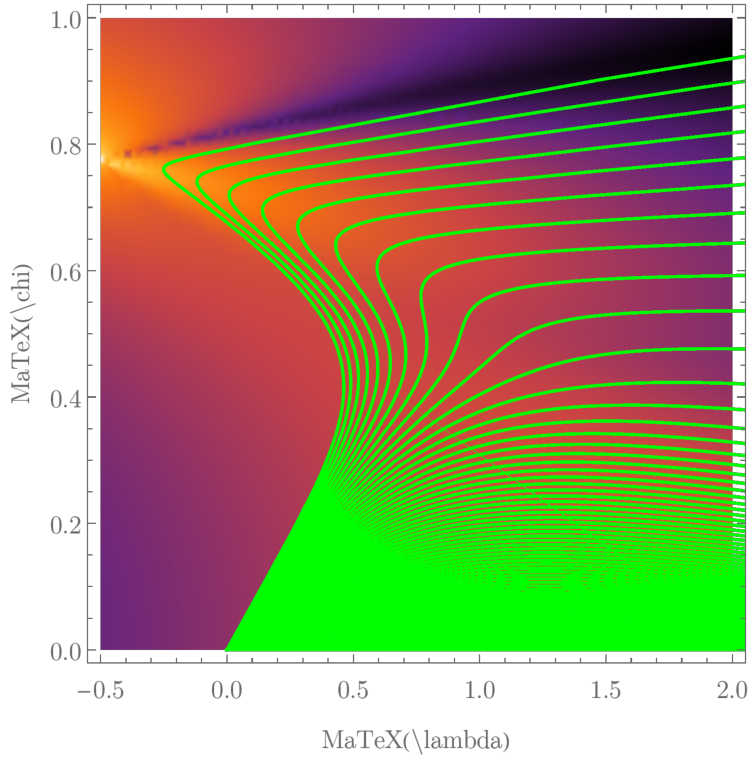
\includegraphics{../img/N=3_geodesics.pdf}
    \begin{tikzpicture}
        \node[anchor=south west,inner sep=0] at (0,0) {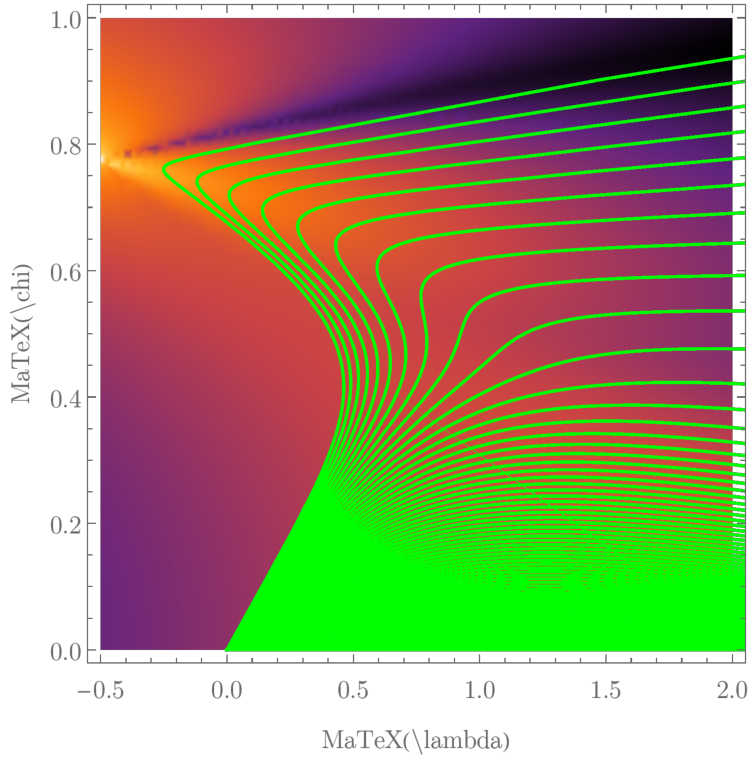
\includegraphics{../img/N=3_geodesics.pdf}};
        \draw[blueee,ultra thick] (4.5,9.56) -- (10.67,10.5);
        \draw[blueee,ultra thick] (4.5,2.71) -- (10.67,1.8);
    \end{tikzpicture}
    \caption{\green{Geodesics} for $N=3$ starting from $(\lambda_i;\chi_i)=(0;0)$ with $(\lambda'_i;\chi'_i)=(\cos\theta;\sin\theta)$, parametrized by angle $\theta\in [-0.63;0.63]$, $\theta\in [\pi-0.225;\pi+0.225]$, with step $\Delta\theta=0.01$. \blueee{Blue} line marks the \blueee{unreachable gap}, where the Ricci curvature is big.}
    \label{fig:N=3_geodesics}    
\end{figure}



\begin{figure}[H]
    \centering
    \begin{tikzpicture}
        \node[] at (0,0) {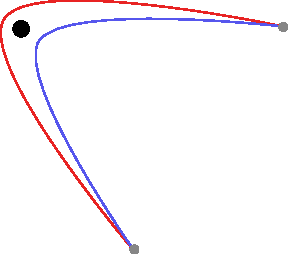
\includegraphics[width=0.3\textwidth]{../img/comparingGeodesics.pdf}};
        \node[] at (-3.2,1.53) {singularity};
        \node[] at (3.0,1.5) {\gray{$(\lambda_i;\chi_i)$}};
        \node[] at (0.8,-1.9) {\gray{$(\lambda_f;\chi_f)$}};        
    \end{tikzpicture}
    \caption{Comparing \gray{boundary} valued geodesics with \blue{repulsing (inner line)} and \red{attracting (outer line)} metric tensor divergence in the spherically symmetrical space. }
    \label{fig:geodesicsinGR}
\end{figure}



% \begin{figure}[h]
%     \centering
%     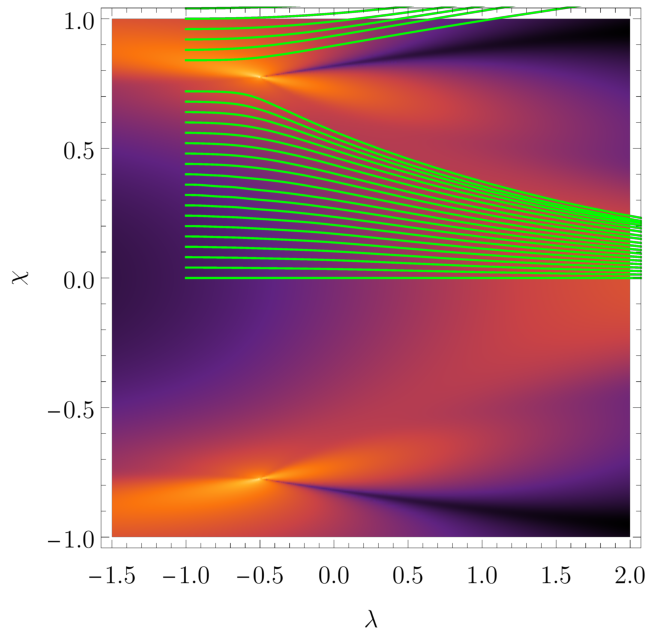
\includegraphics{../img/N=3_geodesics_lambdaIn=-1.pdf}
%     \caption{Geodesics starting from $(\lambda_i;\chi_i)=(-1;\chi_i)$, $(\lambda',\chi')=(1;0)$, for $\chi_i\in(0;1)$ with step $0.05$. Numerically unstable geodesics were skipped. Case $N=3$.}
%     \label{fig:N=3_geodesics_lambdaIn=-1}    
% \end{figure}





\subsection{5-dimensional Hamiltonian}

Another special case is $N=5$. Between every two neighboring energy levels, there are many degeneracies, as can be seen in Fig. \ref{fig:singularitiesBetweenEnergiesN=5}. $E_0=E_1$ degeneracy lies approximately on the line called \emph{separatrix} (see Chap. \ref{chap:infiniteDimensionLimit}) and other singularities are distributed around. The $\chi\leftrightarrow-\chi$ symmetry holds for all of them.


\begin{figure}[H]
    \centering
    \begin{tikzpicture}
        \node[] at (0,0) {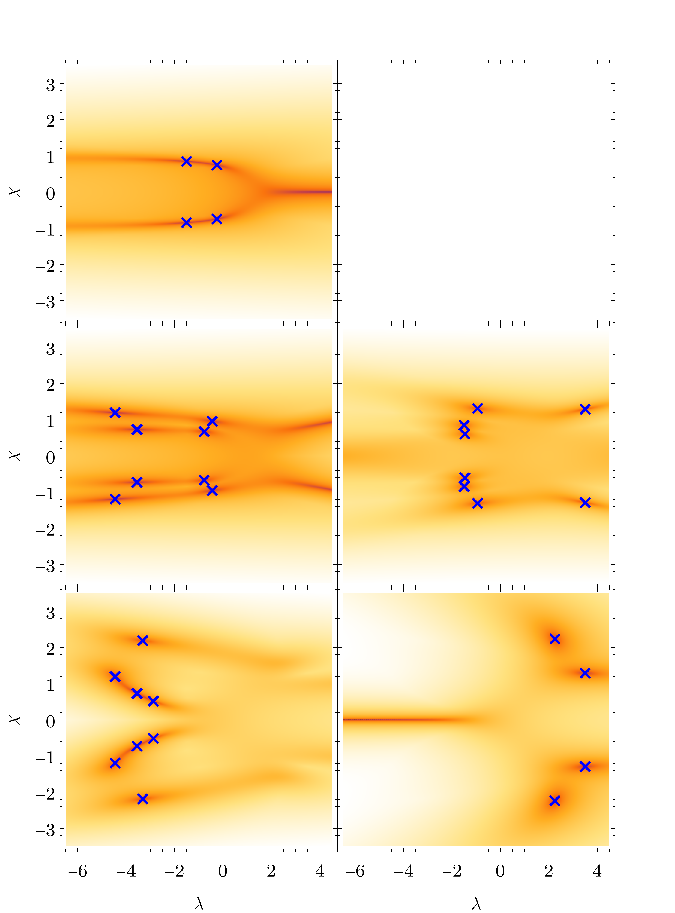
\includegraphics[scale=1.3]{../img/singularitiesBetweenEnergiesN=5.pdf}};
        \node[] at (-1.1,8.2) {$E_1-E_0$};
        \node[] at (-1.1,2.2) {$E_2-E_1$};
        \node[] at (5,2.2) {$E_3-E_2$};
        \node[] at (-1.1,-3.5) {$E_4-E_3$};
        \node[] at (5,-3.4) {$E_5-E_4$};
    \end{tikzpicture}
    \caption{Energy differences between neighboring energy levels for $N=5$. Spectra degeneracies are marked with \blue{blue cross}.
    % First row: $E_1-E_0$, second row from left: $E_2-E_1$, $E_3-E_2$, third row from left: $E_4-E_3$, $E_5-E_4$. 
    }
    \label{fig:singularitiesBetweenEnergiesN=5}   
\end{figure}

The ground state manifold can be understood from the metric tensor determinant, see Fig. \ref{fig:N=5_det3D}. Here we see the spectrum degeneracy causes high positive values of metric tensor determinant and the \blueee{unreachable gap} is characterized by small determinant values. 
\begin{figure}[H]
    \centering
    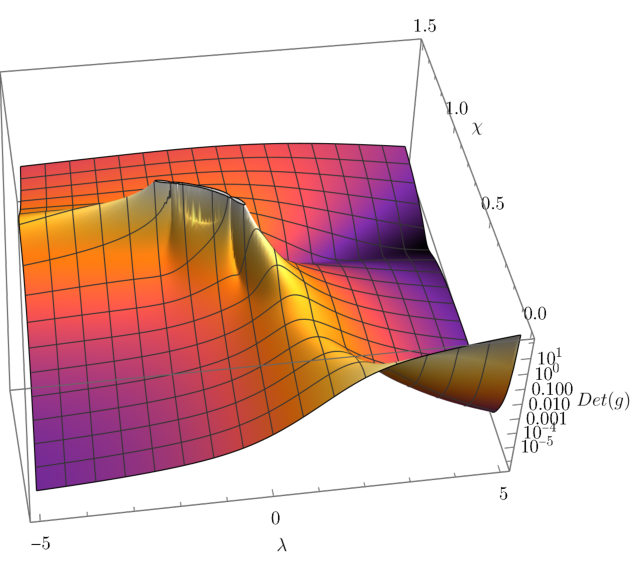
\includegraphics[scale=1.3]{../img/N=5_det3D.pdf}
    \caption{Metric tensor determinant for the case $N=5$.}
    \label{fig:N=5_det3D}    
\end{figure}



Geodesics for case $N=5$ starting at $(\lambda;\chi)=(0;0)$ have the characteristics already seen in the case $N=3$. However, when starting at $(1;0)$, the behavior around the singularity is not the only interesting thing happening. As can be seen in Fig. \ref{fig:geod10}, the geodesics tend to deflect themselves from the area with high curvature around the axis $\chi=0$, which happens even for other initial conditions, just that for $(0;0)$ it is not so apparent. Small irregularity can be seen in Fig. \ref{fig:N=3_geodesics} around point $(0.5;0.1)$ and means that the geodesic equation might have at least two solutions as candidates for the globally shortest path between two points.\footnote{One might recall the effect of gravitational lensing here. In the presence of any mass in spacetime, there exist more possible light paths (solutions to the geodesic equation) between two points, differing by the initial condition.} 



\begin{figure}[H]
    \centering
    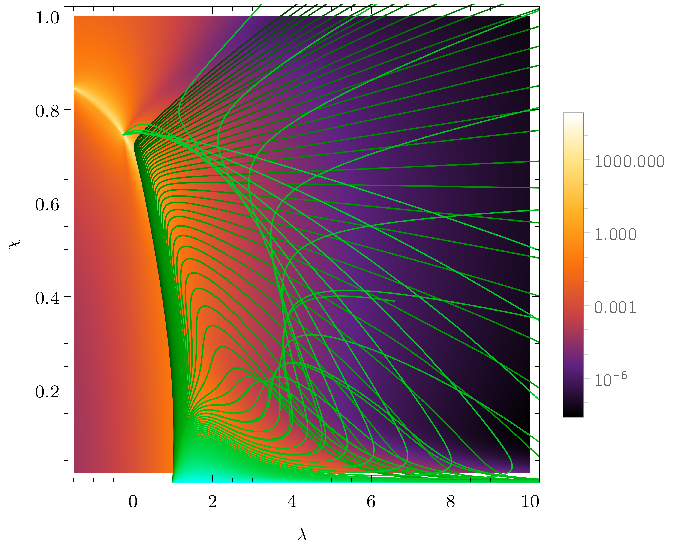
\includegraphics[scale=1.3]{../img/N=5_geods00.pdf}
    \caption{Geodesics for the case $N=5$, starting at $(1;0)$. \emph{The numerics for geodesics passing close to singularity can be observed to break down.}}
    \label{fig:geod10}    
\end{figure}

% \begin{figure}[H]
%     \centering
%     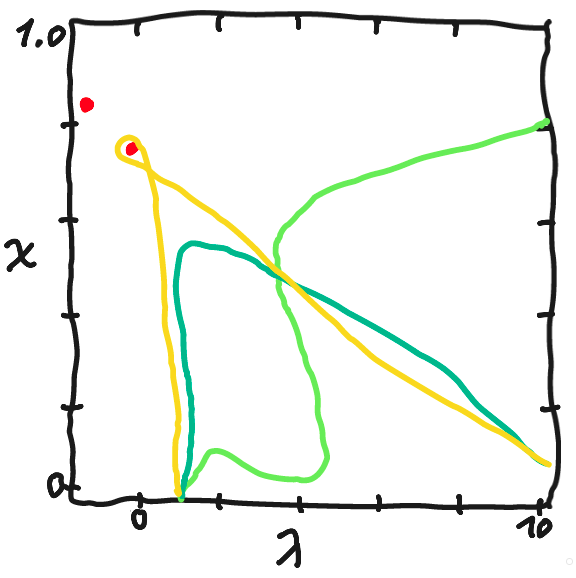
\includegraphics[scale=0.35]{../img/geodesicSolutionsDrawing.png}
%     \caption{Three possible solutions between points $(1;0)$ and $(4;0.5)$. The length of the yellow one is surely longer than other two, but the difference between green vs. blue solution is not clear on the first sight.}
%     \label{fig:geodesicsBetweenPoints}    
% \end{figure}






\subsection{Infinite dimension limit}
\label{chap:infiniteDimensionLimit}
The limit $N\rightarrow \infty$ can be taken from Hamiltonian in Eq. \ref{eq:firstOrderTransitionHamiltonian} using Holstein-Primakoff mapping \citet{holstein} for bosonic operators
\begin{equation}
    \mathcal{H}\coloneqq\lim_{j\rightarrow\infty}\frac{\HH}{2j},
\end{equation}
resulting in classical Hamiltonian
\begin{equation}
    \begin{split}
        \mathcal{H}(x,p)=&-\frac{1}{2}+\frac{1-\lambda}{2}x^2+\frac{\lambda-\chi^2}{4}x^4-\frac{\chi x^3}{2}\sqrt{2-x^2-p^2}-\frac{\chi^2}{4}p^4\\
        &+\frac{p^2}{4}\left[2+(\lambda-2\chi^2)x^2-2\chi x\sqrt{2-x^2-p^2}\right].
    \end{split}
    \label{eq:HamiltonianClassicalLimit}
\end{equation}
For more, see \citet{felipe}.

The \emph{separatrix} is line, where the minima of function $\H(x,p)$ lies. In this case it can be expressed as
\begin{equation}
    \chi^2=\frac{\lambda-1}{\lambda-2}.
    \label{eq:separatrix}
\end{equation}
The separatrix represents phase transition in the limit $N\rightarrow \infty$. In the case of the LMG model, the transition is of first-order everywhere, except in $(\lambda;\chi)=(1;0)$, where it has order two. The separatrix is shown in Fig. \ref{fig:transitionCompare} compared to minimum of $E_1-E_0$ function line, so-called \emph{minimal line}. With increasing $N$, it converges to separatrix.

\begin{figure}[H]
    \centering
    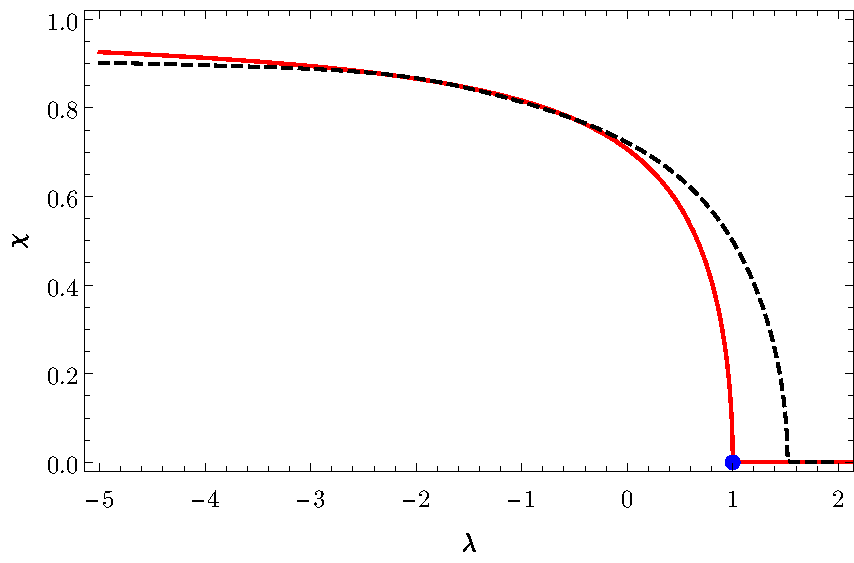
\includegraphics{../img/infiniteN_transitionCompare.pdf}
    \caption{\red{First order phase transition, the separatrix (red line)}, \blue{second order transition (blue point)} compared to \emph{minimal line in N=3 case} (black, dashed).}
    \label{fig:transitionCompare}    
\end{figure}












\section{General spectrum behavior}
For higher dimensions we see the same characteristic behaviour in the energy spectrum sections, see the example in Fig. \ref{fig:N=10_energiesl}, \ref{fig:N=10_energies2} for $N=10$ case. It is not yet clear if there is a degeneracy between every two neighboring energy levels. From numerical observation on $N<10$ goes that there are $N-2$ crossings for $N$ odd and $N-3$ for $N$ even. Here the analytical proof needs to be found.


\begin{figure}[H]
    \centering
    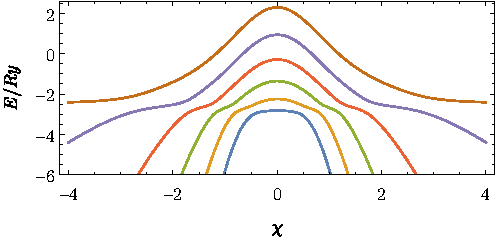
\includegraphics[scale=1.4]{../img/N=10_energiesl.pdf}
    \caption{Energy spectrum as function of $\chi$. $\lambda=1$ and $N=10$.}
    \label{fig:N=10_energiesl}    
\end{figure}
\begin{figure}[H]
    \centering
    \includegraphics[scale=1.4]{../img/N=10_energies2.pdf}
    \caption{Energy spectrum as function of $\lambda$. $\chi=1$ and $N=10$.}
    \label{fig:N=10_energies2}    
\end{figure}

Special attention was given to the spectrum degeneracies between zeroth and first energy level because these influence the metric tensor and ground-state manifold geodesics the most. Their exact calculation is numerically expensive, and only the first few cases, namely, $N\in\{3,4,5,6,7\}$, were calculated, see Tab. \ref{tab:singularities}. 
\begin{table}[H]
    \centering
    \begin{tabular}{c||c|c|c}
     N&$(\lambda_l;\pm\chi_l)$&$(\lambda_2;\pm\chi_2)$&$(\lambda_r;\pm\chi_r)$        \\ \hline\hline
     3&$(-\frac{1}{2};\sqrt{\frac{3}{5}}) $&                                       &                                         \\
     4&$(-3          ;\sqrt{\frac{4}{5}}) $&                                       & $(-\frac{1}{3};\sqrt{\frac{4}{7}})$     \\
     5&$(-\frac{3}{2};\sqrt{\frac{5}{7}}) $&                                       & $(-\frac{1}{4};\sqrt{\frac{5}{9}})$     \\
     6&$(-5          ;\sqrt{\frac{6}{7}}) $&$(-1          ;\sqrt{\frac{2}{3}}) $   & $(-\frac{1}{5};\sqrt{\frac{6}{11}})$     \\
     7&$(-\frac{5}{2};\sqrt{\frac{7}{9}}) $&$(-\frac{3}{4};\sqrt{\frac{7}{11}}) $  & $(-\frac{1}{6};\sqrt{\frac{7}{13}})$ 
    \end{tabular}
    \caption{Singularities between the zeroth and first energy levels for dimensions 3--7. Subscript $l(r)$ means the most \emph{left(right)-wise} positioned coordinates in the $(\lambda,\chi)$-plot.}
    \label{tab:singularities}
    \end{table} 

From singularity behavior in low dimensions, one might see the pattern for $(\lambda_l,\chi_l)$ and $(\lambda_r,\chi_r)$, i.e., those with minimal, resp maximal $\lambda$ coordinate
\begin{equation}
    (\lambda_l ;\pm\chi_l)= \begin{cases}
        \left(1-\frac{N}{2};\sqrt{\frac{N}{N+2}}\right) & , N\geq 3,N\text{ is odd}\\
        \left(1-N;\sqrt{\frac{N}{N+1}}\right) & , N\geq 3,N\text{ is even}
    \end{cases}
    \label{eq:singularityCoordinateFormulaLeft}
\end{equation}
\begin{equation}
    (\lambda_r ;\pm\chi_r)= 
        \left(\frac{1}{1-N};\sqrt{\frac{N}{2N-1}}\right)\quad , N\geq 3.
        \label{eq:singularityCoordinateFormulaRight}
\end{equation}
These were numerically proven to be singularities for cases up to $N=1000$. 

Dimensions 3 to 10 are shown in Fig. \ref{fig:singularities3to10}.
In addition, the degeneracies between zeroth and first energy levels belong to the separatrix described by Eq. \ref{eq:separatrix}. Due to this, the position of singularities is constrained to the \emph{second order phase transition line} between points $(\lambda_l,\pm\chi_l)$ and $(\lambda_r,\pm\chi_r)$.



In the limit $N\rightarrow\infty$ they converge to
\begin{align*}
    \lim_{N\rightarrow \infty}(\lambda_l ;\pm\chi_l)&= \left(-\infty,1\right)\\
    \lim_{N\rightarrow \infty}(\lambda_r ;\pm\chi_r)&= \left(0,\frac{1}{\sqrt{2}}\right).
\end{align*}

It is still unclear if in the limit $N\rightarrow \infty$ the singularities cover the part of separatrix with $\lambda<0$.

\begin{figure}[H]
    \centering
    \includegraphics[scale=1.3]{../img/singularitiesPlots.pdf}
    \caption{Spectrum degeneracies between $E_0$ and $E_1$. Hamiltonian dimensions are 1,3,5,7 in the first column and 2,4,6,8 in the second column. Black crosses mark most left-wise and right-wise singularity and the background corresponds to the metric tensor determinant. Other singularities are also well visible in the determinant as defects on the \emph{high determinant value line}.}
    \label{fig:singularities3to10}    
\end{figure}









% \section{Higher state manifolds}



% \begin{figure}[H]
%     \centering
%     \includegraphics[scale=1.2]{../img/N=5_metricDeterminants.pdf}
%     \includegraphics[scale=1.2]{../img/N=3_barA.pdf}
%     \caption{Arctangens of the metric tensor for higher state manifolds. By  rows: $M_0$, $M_1$; $M_2$, $M_3$; $M_4$, $M_5$.}
%     \label{fig:higherStateManifolds}    
% \end{figure}


% \begin{figure}[H]
%     \centering
%     \includegraphics[width=1\textwidth]{../img/fidelity_lineVSgeodesic.pdf}
%     \includegraphics[width=0.8\textwidth]{../img/fidelity_geodesicVSline_fuckedupcolors.png}
%     \caption{\textcolor{gray}{Infidelity difference between line and geodesic, above picture is original from Felipe, bottom one is edited in GIMP to see the difference more clearly.}}
%     \label{fig:higherStateManifolds}    
% \end{figure}

\chapter{Driving on the ground state manifold}
Of special importance in theory of the ground state manifold are geodesics. It is not yet clear what role they have in general, but in some special cases its well known, see \cite{polkovnikov}. The holy grail of this theory would be to find path with the lowest excitation amplitude, which is not an easy task.

Let's have a geodesic $\mathcal{G}(t)$ and some curve $\gamma(t)$ on the ground stat manifold, spanning between points $P_i$ and $P_f$ during some time $t_f$, meaning
 $$\mathcal{G}(0)=\gamma(0)=P_i\in\mathcal{M}_0,\qquad \mathcal{G}(t_f)=\gamma(t_f)=P_f\in\mathcal{M}_0.$$

Excitation amplitude during infinitesimal quench is $\d s$, therefore $\sum_i \Delta s_i$ summed along path $\gamma(t)$ is the amplitude of transport along that path. This can be more rigorously expressed by functional
\begin{equation}
    s_\gamma=\int_{\gamma(t)}\d s=\int_{0}^{t_f}\sqrt{g_{\mu\nu}\dot\lambda^\mu\dot\lambda^\nu}\d t
\end{equation}
This is the entity, which is minimal if $\gamma$ is a geodesic. Before moving on, lets quickly review the proof of this statement.

\begin{proof}[Geodesics minimize the distance on manifold]
    Functional of distance is
    \begin{equation}
        s=\int\mathcal{L}(t,\lambda^\mu,\dot\lambda^\mu)\d t
    \end{equation}
    for 
    \begin{equation}
        \mathcal{L}=\sqrt{g_{\mu\nu}\dot\lambda^\mu\dot\lambda^\nu}.
    \end{equation}
    Using Euler-Lagrange equations 
    \begin{equation}
        \der{\mathcal{L}}{\lambda^\mu}-\der{}{t}\der{\mathcal{L}}{\dot\lambda^\mu}=0,
    \end{equation}
    we get for $g_{\mu\nu}=g_{\mu\nu}(\lambda^\mu)$ second order differential equation
    \begin{equation}
        \ddot\lambda^\mu+\Gamma^\mu_{\;\;\alpha\beta}\dot\lambda^\alpha\dot\lambda^\beta=0\qquad \Gamma^\mu_{\;\;\alpha\beta}=\frac{1}{2}g^{\mu\kappa}\left(g_{\kappa\alpha,\beta}+g_{\kappa\beta,\alpha}-g_{\beta\alpha,\kappa}\right),
        \label{eq:geodesicEquaiton}
    \end{equation}
    which is the Geodesic equation.
\end{proof}

Excitation probability along the path $\gamma$ can be formally written as $F=\sum_i\Delta s_i^2$, which cannot be simply calculated as $s^2$. Because $\Delta s_i>0$, we have
\begin{equation}
    \begin{split}
        \sum_i \Delta s_i^2& <(\sum_i\Delta s_i)^2\\
        F&<s^2.
    \end{split}
\end{equation}

This doesn't necessarily mean, that fidelity along geodesic will be minimal ($F(\mathcal{G})<F(\gamma)$), because we didn't rule out the scenario 
$$F(\gamma)<F(\mathcal{G})<s_\mathcal{G}^2<s_\gamma^2.$$

This means, that the geodesic equation cannot be used for fidelity minimization and some new insight is needed. The functional, which needs to be minimized is
\begin{equation}
    F=\int\int g_{\mu\nu}\d\lambda^\mu\d\lambda^\nu = \int_{t_i}^{t_f}\underbrace{\int_{t_i}^\tau g_{\mu\nu}\der{\lambda^\mu}{t}\der{\lambda^\nu}{t} \d t}_{\mathcal{L}(\lambda^\mu,\dot\lambda^\mu,\tau)}\d \tau .
\end{equation}
Using Euler-Lagrange equations, again for time independent $g_{\mu\nu}=g_{\mu\nu}(\lambda^\mu)$, leads to
\begin{equation}
    \int_{t_i}^{t_f}\left[g_{\mu\nu,\kappa}\dot\lambda^\mu\dot\lambda^\nu - \der{}{t}\left[g_{\mu\nu}\left(\delta^\mu_\kappa\dot\lambda^\mu+\dot\lambda^\mu\delta^\nu_\kappa\right)\right]\right]\d t=0
\end{equation}
which needs to be zero for integration over any subset $(t_i,t_f)$ leading to zero condition for the integrand itself, which leads to geodesic equation \ref{eq:geodesicEquaiton}, as in the case of distance on manifold.



\textcolor{blue}{Polkovnikov for some special case: They play a role of "maximum fidelity at any time" transport, meaning at any given time $t$ the fidelity on corresponding point on geodesics will be less than of $\gamma$
$$F(\mathcal{G}(t))<F(\gamma(t)).$$ }









\section{The role of geodesics}


\subsection{Minimizing the energy variance}
From \cite{Bukov2019}.
About transports using \emph{fast forward} Hamiltonian means the system is driven to the target state in some fixed amount of time. The transport is done on the ground state manifold $\M$.

\conjecture{
    For any fast forward Hamiltonian $\HH(\lambda(t))$ driven along one dimentional path $\lambda(t): \R\mapsto \R$ using time $t$ as parametrization, the energy fluctuations $\delta E^2$, averaged along the path, are larger than the geodesic length $l_\lambda$
    \begin{equation}
        \int\limits_0^T\sqrt{\delta E^2(t)}\d t \eqqcolon l_t\geq l_\lambda \int\limits_{\lambda_i}^{\lambda_f} \sqrt{g_{\lambda\lambda}} \d \lambda=\int_0^T \sqrt{g_{\lambda\lambda}}\frac{\d \lambda}{\d t}\d t.
    \end{equation}
    The length $l_\llambda$ is defined in control space (with metric tensor $g_{\lambda\lambda}$) and is generally larger than the distance between wave functions, i.e. the absolute geodesic (defined with $G_{\mu\nu}$). From its definition, we can see that it corresponds to the metric tensor as we use it.
    
    
    
    The energy variance is 
    \begin{equation}
        \delta E^2= \braket{o(t)|\HH(t)^2|o(t)}-\braket{o(t)|\HH(t)|o(t)}^2=\braket{\partial_t (t)|\partial_t o(t)})_c=G_{tt}
    \end{equation}    
    and the Metric tensor in control space is defined as
    \begin{equation}
        g_{\lambda\lambda}\coloneqq \braket{\partial_\lambda o(t)|\partial_\lambda o(t)})_c
    \end{equation}
}


\begin{proof}
    \begin{equation}
        \delta E^2\equiv \braket{o(t)|\HH(t)^2|o(t)}_c=\dot\lambda^2 G_{\lambda\lambda}+\O(\dot\lambda^4),
    \end{equation}
    where $\O(\dot\lambda^4)$ needs to be positive for any real-valued Hamiltonian. This comes from the fact, that it has instantaneous time-reversal symmetry.
\end{proof}

The conjecture only applies to unit fidelity protocols ($F(t)=1 \;\forall t\in[0,T_f]$) and can be extended to an arbitrary dimensional path.












\section{The meaning of geodesics}


\subsection{Transport using quenches}
\label{sec:quenches}
Unifying the ground states $\ket{o(\llambda)}$ over all points $\llambda\in\R^n$ in the parameter space, we get the ground state manifold. Here the fidelity $f$ and distance $s$ are defined
\begin{equation}
    \d s^2 \equiv 1-f^2\equiv 1-\left|\braket{o(\bm\llambda+\delta\bm\llambda)|o(\bm\llambda)}\right|^2.
    \label{eq:distanceOnM0}
\end{equation}

The final fidelity of transport on $\M$ is then
\begin{equation}
    F=\iint g_{\mu\nu}\d\lambda^\mu\d\lambda^\nu = \int_{t_i}^{t_f}\underbrace{\int_{t_i}^\tau g_{\mu\nu}\der{\lambda^\mu}{t}\der{\lambda^\nu}{t} \d t}_{\mathcal{L}(\lambda^\mu,\dot\lambda^\mu,\tau)}\d \tau .
\end{equation}
Using Euler-Lagrange equations for time-independent $g_{\mu\nu}=g_{\mu\nu}(\lambda^\mu)$, leads to
\begin{equation}
    \int_{t_i}^{\tau}\left[g_{\mu\nu,\kappa}\dot\lambda^\mu\dot\lambda^\nu - \der{}{t}\left[g_{\mu\nu}\left(\delta^\mu_\kappa\dot\lambda^\nu+\dot\lambda^\mu\delta^\nu_\kappa\right)\right]\right]\d t=0,
\end{equation}
which needs to be zero for integration over any subset $(t_i,\tau)$. This can bne achieved for any path only it the integrand itself is zero, which happens if the geodesic equation holds.

The fidelity $f$ measures transition probability between two neighboring eigenstates of two different Hamiltonians. Those two states belong to the same Fibre space $\PH(\llambda)\times \R^n$ from which the coefficients $(\Z,\llambda)$ are taken. Because all $\PH(\llambda)$ are canonically isomorphic, there is no problem in parallel transport from one space to another, which is needed for braket\footnote{This procedure is done without thinking in the back part of our brains such, that we don't even think about it. That's how trivial it is.}.

The distance minimization runs into some interpretation problems. On one hand, minimalization of the distance is equivalent to maximalization of the sum of infinitezimal fidelities along the path (we say we \emph{maximize the fidelity along the path}). On the other hand we are using only ground states in every step of the transport, therefore defining the fidelity to be one. There are actually two ways out of this confusion. \emph{Perturbed adiabatic driving} and \emph{Transport using quenches}.


\subsubsection{Perturbed adiabatic driving}
It the first case, we imagine at every point of transport, that the fidelity is small enough, such that in eigenbasis and some small parameters $\delta_i\in \mathbb{C}$ we get
$$\ket{o(\llambda_i)}\equiv \begin{pmatrix}
    Z_0(\llambda_i)\\
    0\\
    \vdots \\
    0
\end{pmatrix} \overset{\text{transport }\d s}{\longrightarrow} \ket{o(\llambda_i+\delta \llambda)}\equiv\begin{pmatrix}
    Z_0(\llambda_i+\delta \llambda)\\
    0\\
    \vdots \\
    0
\end{pmatrix} +\underbrace{\begin{pmatrix}
    0\\
    \delta_1(\llambda_i+\delta \llambda)\\
    \vdots \\
    \delta_n(\llambda_i+\delta \llambda)
\end{pmatrix}}_{\mathbf{\Delta}(\llambda_i+\delta \llambda)}, $$
where the last term is neglected using 
$$\braket{\Delta(\llambda)|o(\llambda+\delta\llambda)}\approx 0.$$

This might have interesting implication for slow transports, or small distance transports. For example when some slow thermalization is considered during a transport.









\section{Transport using quenches}
If we imagine $\delta\llambda$ to be finite (not infinitely small, as the notation suggests), the \textbf{transport} means \textbf{doing a sequence of quenches and measuring the system after every quench}.


Some notion of the space of our Hamiltonian can be seen by quenching from $(\lambda_i;\chi_i)=(0;0)$ to $(\lambda;\chi)$, as can be seen in Figure \ref{fig:quenchFidelityFrom00}.

In Figure \ref{fig:equidistantPointsOnPath} are marked equidistant points, meaning $\int_a^b \d s=\text{const.}$ between every two neighboring points on curve. This means that if the system is measured periodically, the quenches jump smaller distances when closer to a singularity.

Decreasing time step $\Delta t$ has no effect on the relative fidelity of quenches during the evolution but has an effect on their magnitude. As one would expect from \emph{quantum Zeno effect}, when $\Delta t\rightarrow 0$, the transport becomes adiabatic, and the fidelity at any time will become 1. This can be observed in Figure \ref{fig:plotsFidelityQuenches}, such that the shape of the point-like paths looks similar in the columns, and their magnitude decreases.

The quantum Zeno effect for this case can be shown dirrectly by splitting the distance $s$ to $N$ equal pieces. The fidelity for $N$ splits will then be
\begin{equation}
    f(N)=(1-\Delta s)^N=\left(1-\left(\frac{s}{N}\right)^2\right)^N \;\;\overset{N\rightarrow\infty}{\longrightarrow}\;\; 1,
\end{equation}
meaning the consequent measurements will colapse the system to its instantenous eigenstate and the adiabatic condition for transport holds. 

Such measurements can be achieved by fast thermalization of the system. If the finite speed thermalization with $N=T/\tau$ for the mean time between two measurements $\tau$, we get
\begin{equation}
    \begin{split}
        \log f(N) &= N \log \left(1-\left(\frac{s}{N}\right)^2\right) = -\frac{s^2}{N}+o\left(\frac{s^4}{n^3}\right)\\
        f(N) &= \exp\left(-s^2\frac{\tau}{T}-\frac{s^4}{2 N^3}\dots\right) = \exp\left(-s^2\frac{\tau}{T}\right)\left(1+o\left(\frac{s^4}{N^3}\right)\right)
    \end{split}
\end{equation}


\begin{figure}[H]
    \centering
    \includegraphics[scale=1.2]{../img/quenchFidelityFrom00.pdf}
    \caption{Arctangens of the fidelity of quenches from $(\lambda_i;\chi_i)=(0;0)$ to $(\lambda;\chi)$.}
    \label{fig:quenchFidelityFrom00}    
\end{figure}

\begin{figure}[H]
    \centering
    \includegraphics[scale=1.2]{../img/equidistantPointsOnPath.pdf}
    \caption{Equidistant points on geodesics of the ground state manifold.}
    \label{fig:equidistantPointsOnPath}    
\end{figure}

\begin{figure}[H]
    \centering
    \includegraphics[scale=1.2]{../img/bg123.pdf}
    \includegraphics[scale=0.6]{../img/plotsFidelityQuenches.pdf}
    \caption{Fidelity for sequential quenches along geodesics (see green lines on top). Left (right) column corresponds to lower (upper) geodesic. Time steps from top are $\Delta t\in \{0.03,0.1,0.5\}$. Time difference between points in the plot on top is $\Delta t=0.5$.}
    \label{fig:plotsFidelityQuenches}    
\end{figure}





\chapter*{Conclusion}
\addcontentsline{toc}{chapter}{Conclusion}
This thesis presents the theory of quantum state driving theory of finite Hamiltonian systems. The well known claims were reformulated into more rigorous theorems and definitions style of writing. This mathematical approach has potential to reduce the barrier for any mathematically based scientist without training in quantum mechanics when trying to approach this theory. The playground in the form of fiber space was constructed, and the geometry of energy states reformulated on it. Some theorems were proposed based on previous knowledge from the area of physics concerning quantum state driving, and clear definitions of generally used terms were presented.

The correspondence to a damped harmonic oscillator in the fidelity behavior was shown on a simple two-level system. In the case of geodesic driving, the fidelity oscillates with constant frequency and periodically becomes one. For linear driving, the fidelity has essentially two regimes — fast transport regime, described by the semiclassical Landau-Zener formula, and close adiabatic regime, described by APT. In both models, the fidelity is excited when the difference between energy levels gets small. These excitations lead to damped oscillations.

In the LMG model, the ground state manifold is analyzed. The Riemannian manifold characteristics were calculated along with their implications. These are ground state manifold geodesics and coordinates of diabolic points in parametric space, dependent on the Hamiltonian dimension. In three dimensions, this was done analytically, proving the existence of diabolic points. For higher dimensions, numerical methods were used. The transport using quenches was numerically demonstrated, showing the transformation to adiabatic transport by shortening the quenches.

Many questions still lay unsolved, and some were newly opened. For example: "What are the possibilities for quantum quench transport?". "What is the correspondence of energy variance and driving fidelity?". Further on, from the LMG model, the proposed analytical formula for diabolic points coordinates remains to be proven analytically, along with the number of these points.

This thesis provides a significant amount of numerical analysis on two quantum models, which will hopefully serve for future discoveries in this area of physics. The state manifold analyses might lead the search for better fidelity protocols, or maybe the geodesics will be found to be somewhat "most stable protocols" for counter-diabatic driving. Either way, the possibilities are yet open and not known.

%%% Bibliography
%%% Bibliography (literature used as a source)
%%%
%%% We employ bibTeX to construct the bibliography. It processes
%%% citations in the text (e.g., the \cite{...} macro) and looks up
%%% relevant entries in the bibliography.bib file.
%%%
%%% The \bibliographystyle command selects, which style will be used
%%% for references from the text. The argument in curly brackets is
%%% the name of the corresponding style file (*.bst). Both styles
%%% mentioned in this template are included in LaTeX distributions.
\bibliographystyle{unsrtnat}
% \bibliographystyle{plainnat}    %% Author (year)
% \bibliographystyle{unsrt}     %% [number]

\renewcommand{\bibname}{Bibliography}

%%% Generate the bibliography. Beware that if you cited no works,
%%% the empty list will be omitted completely.

\bibliography{bibliography}

%%% If case you prefer to write the bibliography manually (without bibTeX),
%%% you can use the following. Please follow the ISO 690 standard and
%%% citation conventions of your field of research.

% \begin{thebibliography}{99}
%
% \bibitem{lamport94}
%   {\sc Lamport,} Leslie.
%   \emph{\LaTeX: A Document Preparation System}.
%   2nd edition.
%   Massachusetts: Addison Wesley, 1994.
%   ISBN 0-201-52983-1.
%
% \end{thebibliography}


%%% Figures used in the thesis (consider if this is needed)
\listoffigures

%%% Tables used in the thesis (consider if this is needed)
%%% In mathematical theses, it could be better to move the list of tables to the beginning of the thesis.
%\listoftables

%%% Abbreviations used in the thesis, if any, including their explanation
%%% In mathematical theses, it could be better to move the list of abbreviations to the beginning of the thesis.
%\chapwithtoc{List of Abbreviations}

%%% Attachments to the master thesis, if any. Each attachment must be
%%% referred to at least once from the text of the thesis. Attachments
%%% are numbered.
%%%
%%% The printed version should preferably contain attachments, which can be
%%% read (additional tables and charts, supplementary text, examples of
%%% program output, etc.). The electronic version is more suited for attachments
%%% which will likely be used in an electronic form rather than read (program
%%% source code, data files, interactive charts, etc.). Electronic attachments
%%% should be uploaded to SIS and optionally also included in the thesis on a~CD/DVD.
%%% Allowed file formats are specified in provision of the rector no. 72/2017.
\appendix
\chapter{Geometrization of quantum mechanics}
\label{appendixGEOM}
Differential geometry is believed to be the modern language of physics, and there is a strong urge to reformulate theories in this language. As introduction to the problem, see \citet{ashtekar_geometrical_1997}, \cite{ashtekar_geometry_1995}, or more mathematical work by \citet{molitor_exponential_2013}.

The whole thesis uses a classical formulation of quantum mechanics with some parts described using differential geometry. Here, the complete reformulation of quantum mechanics and the bridge between this theory and the already formulated are introduced. Reformulating the whole theory of quantum driving into the language of differential geometry might give some new insights, but it is beyond the scope of this thesis.


\section{From the projective Hilbert space to state manifolds}


Consider the Hilbert space $\H$ to be a space of \emph{bare states} and $\mathcal{S}$ to be the space of \emph{normalized bare states}. Physical observables are related to the \emph{space of rays}, defined as $\PH\coloneqq \mathcal{H}/U(1)$, for the factorization by elements of one-dimensional unitary group $U(1)$. This group consists of unitary transformations $e^{i\varphi}$ for $\varphi\in\R$, defining gauge symmetry between quantum states. $\PH$ is then considered to be the \emph{space of pure states}. We will consider the states to be normalized, leading to the \emph{space of normalized pure physical states}. 

It can be shown that $\PH$ is of K\"ahler structure, meaning it has two non-degenerate sesquilinear\footnote{Complex conjugated is the first input of the 2-form.} 2-forms embedded along with complex unit operator $J$, defining structure
$$(J, G, \Omega),$$
such that
\begin{equation}
    J^2=\Id.
\end{equation}
Any bracket of $\ket{\psi_1},\ket{\psi_2}\in \PH$ can be decomposed into real and imaginary part\cite{ashtekar_geometrical_1997}
\begin{equation}
    \braket{\psi_1|\psi_2}\equiv Q(\psi_1,\psi_2)=\frac{1}{2}G(\psi_1,\psi_2)-\frac{i}{2}\Omega(\psi_1,\psi_2).
\end{equation}

From braket, sesquilinearity goes that $G$ is symmetric and $\Omega$ antisymmetric form thus they can be uniquely written into one 2-form called \emph{Fubini-Study metric} with property
\begin{equation}
    G=\Re Q ;\qquad \Omega=\Im Q.
\end{equation}

Because $|\braket{\psi_1|\psi_2}|\in[0,1]$ we say, that the \emph{metric is measuring the geodesic distance on the Bloch sphere}. Here if we define
\begin{equation}
    |\braket{\psi_1|\psi_2}|=\cos^2 \frac{\theta}{2},
\end{equation}
we get $\d \theta= 2\d s=2\sqrt{|g_{\mu\nu}\d \llambda^\mu\d \llambda^\nu|}$, see the paper from \citet{cheng_quantum_2013}.

To write the metric in a standard form, we need to realize how our space looks like. For finite $(N+1)$-dimensional Hilbert space, one dimension is lost in the gauge transformation, leaving us with $N$-dimensional $\PH$. Another dimension is lost due to normalization, which is usually done by mapping to an n--dimensional complex sphere
$$CP^N= \left\{ \bm Z=(Z_0,Z_1,\dots,Z_N)\in \mathbb{C}^{N+1}/\{0\} \right\}\Big/ \{\bm Z\sim c\bm Z \text{ for } c\in \mathbb{C}\}.$$

Natural property of such complex spaces is splitting of its tangent space to holonomous and anholonomous part\footnote{The line over index means complex conjugation.}
$$\mathcal T^1_0\M=\Span\left\{\frac{\partial}{\partial Z_i}\right\}; \qquad \mathcal T^0_1\M=\Span\left\{\frac{\partial}{\partial Z_{\overline{i}}}\right\}.$$
For suitable distance $\d Z$, this can be used to define distance on state manifolds.


Distance on $\mathbb{C}^{n+1}$ is usually defined using Hermitian metric\footnote{Hermitian metric is by definition sesquilinear, as one would expect in quantum mechanics later on.} 
\begin{equation}
    \d s^2 = \d \overline{\Z} \otimes \d \Z.
\label{eq:metricdistancePH}
\end{equation}


% For \emph{normalized states} in quantum mechanics is $\d Z=(1, \ket{\d z})^T$, which plugged into Eq. \ref{eq:metricdistancePH} yields
% \begin{equation}
%     \d s^2 = 1-\left|\braket{\psi+\delta \psi|\psi}\right|^2.
%     \label{eq:distanceInPH}
% \end{equation}


\section{Restriction to eigenstate manifolds}
In quantum mechanics, one can examine a Hamiltonian $\HH(\llambda)$, for some parameter $\llambda\in \mathcal U\subset \R^n$. At every point $\llambda$ we get projective Hilbert space $\PH(\llambda)$. This creates a fiber structure space, in which there are some sections with interesting physical applications. Some of these sections are \emph{eigenstate manifolds}, defined by setting only one non-zero coefficient $Z_k$ in eigenbasis $\ket{\psi}=\sum_{k=0}^n Z_k \ket{k}$. From normalization goes automatically $Z_k=1$. The distance on these manifolds is, as derived in Eq. \ref{eq:distanceOnM0},
\begin{equation}
    \begin{split}
        \d s^2 &= \textcolor{gray}{1}-\bra{k+\delta k}\textcolor{gray}{k\rangle \langle k}\ket{k+\delta k}=\textcolor{gray}{1}-\bra{k+\delta k}\textcolor{gray}{\big(\Id-\sum_{j\neq k} \ket{j}\bra{j}\big)}\ket{k+\delta k} \\
        &= \textcolor{gray}{\sum_{j\neq k}}\bra{k+\delta k}\textcolor{gray}{j\rangle \langle j}\ket{k+\delta k}.
        \label{eq:dsDerivation}
    \end{split}
\end{equation}
Using the \Schrodinger equation $\textcolor{blue}{\HH}\ket{k}=\textcolor{teal}{E_k} \ket{k}$, distributivity of derivative and projection to some state $\textcolor{gray}{\bra{j}}$, we get
\begin{equation}
    \begin{split}
        \textcolor{blue}{\HH}\ket{k} &= \textcolor{teal}{E_k}\ket{k}\\
        \textcolor{blue}{(\delta \HH)}\ket{k} +\textcolor{blue}{\HH}\ket{k+\delta k} &=\textcolor{teal}{(\delta E_k)}\ket{k} +\textcolor{teal}{E_k}\ket{k+\delta k}\\
         \textcolor{gray}{\bra{j}}\big(\textcolor{blue}{\delta \HH}-\textcolor{teal}{\delta E_k}\big)\ket{k}&=\textcolor{gray}{\bra{j}}\big(\textcolor{teal}{E_k}-\textcolor{blue}{\HH}\big)\ket{k+\delta k}=\textcolor{gray}{\bra{j}}\big(\textcolor{teal}{E_k}-\textcolor{blue}{E_j}\big)\ket{k+\delta k}.
    \end{split}
\end{equation}
We can set
%\footnote{\textcolor{red}{Can it be done only for $E_0$? It does not make sence generally, because $E=E(\llambda)$, even $E_0=E_0(\llambda)$}} 
$\textcolor{blue}{\delta E_k}=0$, leading for $j\neq k$ to
\begin{equation}
    \frac{\textcolor{gray}{\bra{j}}\textcolor{blue}{\delta \HH}\ket{k}}{(\textcolor{teal}{E_k}-\textcolor{blue}{E_j})^2}=\textcolor{gray}{\langle j}\ket{k+\delta k}.
    \label{eq:braket_k,deltaj}
\end{equation}
Plugging to Equation \ref{eq:dsDerivation} and considering $\HH=\HH(\llambda)$, we get metric on a ground state manifold
\begin{equation}
    \d s^2 = \Re\textcolor{gray}{\sum_{j\neq k}} \frac{\bra{0}\textcolor{blue}{\partial_\mu \HH \textcolor{gray}{\ket{j}}}\textcolor{gray}{\bra{j}}\textcolor{blue}{\partial_\nu \HH}\ket{0}}{(\textcolor{teal}{E_k}-\textcolor{blue}{E_j})^2}  \d \llambda^\mu\d \llambda^\nu.
    \label{eq:distanceonM}
\end{equation}


Definition of the k--state manifold is then
\begin{equation}
    g_{\mu\nu}^{(k)} = \Re \sum_{j\neq k}\frac{\braket{k|\pder{\HH(\llambda)}{\lambda^\mu}|j}\braket{j|\pder{\HH(\llambda)}{\lambda^\nu}|k}}{(E_k-E_j)^2}.
    \label{eq:metrictensork}
\end{equation}
The Fubini-Study metric on the eigenstate manifold is sometimes called \emph{Geometric tensor}. 

\chapter{Eigenvalues for Lipkin-Meshkov Glick model}
\label{appendix1}
Eigenvalues for $N=3$ case of Lipkin-Meshkov Glick model are
\begin{align}
    E_0 &= \frac{1}{12} \left(G-F-\frac{\sqrt{D-E}}{2}\right)\\
    E_1 &= \frac{1}{12}  \left(G-F+\frac{\sqrt{D-E}}{2}\right)\\
    E_2 &= \frac{1}{12} \left(G+F-\frac{\sqrt{D+E}}{2}\right)\\
    E_3 &= \frac{1}{12}  \left(G+F+\frac{\sqrt{D+E}}{2}\right),
\end{align}
for
\begin{equation}
    \begin{split}
    A &= 16 \sqrt[3]{2} \Big(64 \lambda ^6-192 \lambda ^5 \chi ^2+24 \lambda ^4 \left(52 \chi ^4-93 \chi ^2+36\right)\\
    &-8 \lambda ^3 \left(29 \chi ^4+414 \chi ^2-513\right) \chi ^2
    \\
    &+6 \lambda ^2 \left(1225 \chi ^8-10053 \chi ^6+17595 \chi ^4-10557 \chi ^2+1377\right)\\
    &+\bigg(\big(64 \lambda ^6+864 \lambda ^4+8262 \lambda ^2+3 (818 \lambda -27285) \chi ^{10}\\
    &+6 (\lambda  (1225 \lambda -3198)+27108) \chi ^8\\
    &-(2 \lambda  (\lambda  (116 \lambda +30159)-89073)+326727) \chi ^6\\
    &+6 (\lambda  (\lambda  (8 \lambda  (26 \lambda -69)+17595)-42660)+51516) \chi ^4\\
    &-3 (2 \lambda  (\lambda  (4 \lambda  (\lambda  (8 \lambda +93)-171)+10557)-16119)+36207) \chi ^2\\
    &+24013 \chi ^{12}+25515\big)^2\\
    &-\big(16 \lambda ^4+144 \lambda ^2+2 (74 \lambda -1185) \chi ^6+3 (4 \lambda  (16 \lambda -77)+1329) \chi ^4\\
    &-2 (2 \lambda  (\lambda  (8 \lambda +93)-207)+1161) \chi ^2+889 \chi ^8+1053\big)^3\bigg)^{1/2}\\
    &+6 \lambda  \big(409 \chi ^8-3198 \chi ^6+29691 \chi ^4-42660 \chi ^2+16119\big) \chi ^2+24013 \chi ^{12}\\
    &-81855 \chi ^{10}+162648 \chi ^8-326727 \chi ^6+309096 \chi ^4\\
    &-108621 \chi ^2+25515\Big)^{1/3}
    \end{split}
\end{equation}

\begin{equation}
    \begin{split}
   B &= \frac{256 \sqrt[3]{2}}{3A} \bigg(16 \lambda ^4+144 \lambda ^2+2 (74 \lambda -1185) \chi ^6+3 (4 \lambda  (16 \lambda -77)\\
   &+1329) \chi ^4-2 (2 \lambda  (\lambda  (8 \lambda +93)-207)+1161) \chi ^2+889 \chi ^8+1053\bigg)
    \end{split}
\end{equation}
\begin{equation}
   C =4 \sqrt{\frac{A}{3 \sqrt[3]{2}}+B+\frac{16}{3} \left(4 \lambda ^2-(4 \lambda +33) \chi ^2+49 \chi ^4+45\right)}\qquad\qquad\quad
\end{equation}
\begin{equation}
    \begin{split}
   D &= -\frac{A}{3 \sqrt[3]{2}}-B-\frac{8}{3} \left(59 \lambda ^2+436 \lambda  \chi ^2+392 \chi ^4+132 \chi ^2-180\right)\qquad\;\;\\
   &+8 \left(5 \lambda +14 \chi ^2\right)^2
    \end{split}
\end{equation}
\begin{equation}
    \begin{split}       
    E &= \frac{9216}{C} \left((\lambda -1) \chi ^4-4 (\lambda -1) \chi ^2+\lambda -2 \chi ^6\right)\\
    F &= \frac{1}{2} \sqrt{\frac{A}{3 \sqrt[3]{2}}+B+\frac{16}{3} \left(4 \lambda ^2-(4 \lambda +33) \chi ^2+49 \chi ^4+45\right)}\qquad\qquad\;\;\;\\
    G &= -5 \lambda -14 \chi ^2
    \end{split}
\end{equation}

% \chapter{Attachments}

% \section{Computing the metric tensor}
% \red{Mathematica code for metric tensor and geodesics??}


% \section{Computing the Geodesics}

% \section{Computing the driving fidelity}

\openright
\end{document}
